\bibliographystyle{genetics}

\newcommand{\E}{\mathbb{E}}
\renewcommand{\P}{\mathbb{P}}
\newcommand{\half}{\tfrac{1}{2}}

\usepackage[authoryear]{natbib}
\bibliographystyle{genetics}
\newcommand{\wbar}{\overline{w}}
% New commands added by Simon:
\newcommand{\eqn}{eqn}
\newcommand{\fis}{F_{\mathrm{IS}}}
\newcommand{\fit}{F_{\mathrm{IT}}}
\newcommand{\fst}{F_{\mathrm{ST}}}
\newcommand{\Wbar}{\overline{W}}
\newcommand{\dNdS}{\nicefrac{d_N}{d_S}}
\newcommand{\graham}[1]{\todo[size=\scriptsize, color=red!50]{#1}}

\newcommand{\nicefrac}[2]{\frac{#1}{#2}}

\newcounter{question}[chapter]  %[section]   %%modified from https://www.sharelatex.com/learn/Counters

%https://tex.stackexchange.com/questions/428652/newenvironment-for-tcolorbox-and-lstlisting

%mybox
%\newtcolorbox[use counter=question]{question}[1]{colback=red!5!white,
%colframe=red!75!black,fonttitle=\bfseries, 
%title= Question~\thequestion. #1}

\newenvironment{question}
{{\bf Question}}
 %   {\begin{center}
 %   Question~ \thequestion. \\

   % \begin{tabular}{|p{0.9\textwidth}|}
  %  \hline\\
  %  }
  %  { 
   % \\\\\hline
   % \end{tabular} 
  %  \end{center}
  {  }



\title{Population and\newline Quantitative \newline Genetics}
\author{Graham Coop}
%  \small $^1$ Department of Evolution and Ecology \& Center for Population Biology,\\
%  \small University of California, Davis.\\
%  \small To whom correspondence should be addressed: \texttt{gmcoop@ucdavis.edu}\\
%  \small This work is licensed under a Creative Commons Attribution 3.0 Unported License.\\
%  \small http://creativecommons.org/licenses/by/3.0/ \\
%  \small i.e. you are free to reuse and remix this work, but please include an attribution to the original.


\date{}
\maketitle
\newpage

%\tableofcontents

\chapter{Introduction}
\newthought{Biological evolution is the change over time in the genetic composition of a population.}\cite{DobzhanskyBook} Our population is made up of a set of interbreeding individuals, the genetic composition of which is made up of the  genomes that each individual carries.  %While at first this definition of evolution seems at odds with the
%common textbook view of the evolution of phenotypes, such as the changing shape
%of finch beaks over generations, it is genetic changes that underpin these
%phenotypic changes.   \\
The genetic composition of the population alters due to the death of individuals or the migration of individuals in or out
of the population. If our individuals vary in the number of children they have, this
also alters the genetic composition of the population in the next generation.
Every new individual born into the population subtly changes the genetic
composition of the population. Their genome is a unique combination of their
parents' genomes, having been shuffled by segregation and recombination during
meioses, and possibly changed by mutation. These individual events seem minor at the level of the population, but it is the accumulation of small changes in aggregate across individuals and generations that is the stuff of evolution. It is the compounding of these small changes over tens, hundreds, and millions of generations that drives the amazing diversity of life that has emerged on this earth.\\

Population genetics is the study of the genetic composition of natural
populations and its evolutionary causes and consequences. Quantitative genetics is the study of the genetic basis of phenotypic variation and how phenotypic changes evolve over time. Both fields are closely conceptually aligned as we'll see throughout these notes. They seek to describe how the genetic and phenotypic composition of populations can be changed over
time by the forces of mutation, recombination, selection, migration, and
genetic drift.  To understand how these forces interact, it is helpful to
develop simple theoretical models to help our intuition. In these notes we will
work through these models and summarize the major areas of population- and quantitative-genetic
theory.\\


\marginnote{``All models are wrong but some are useful.'' -
  \citet{box:79}.}  % https://en.wikipedia.org/wiki/All_models_are_wrong#Quotations_of_George_Box
% http://www.dtic.mil/dtic/tr/fulltext/u2/a070213.pdf

While the models we will develop will seem na\"{\i}ve, and indeed they are, they are
nonetheless incredibly useful and powerful. Throughout the course we will see
that these simple models often yield accurate predictions, such that much of our
understanding of the process of evolution is built on these models. We will
also see how these models are incredibly useful for understanding real patterns
we see in the evolution of phenotypes and genomes, such that much of our
analysis of evolution, in a range of areas from human medical genetics to conservation,
is based on these models. Therefore, population and quantitative genetics are key to
understanding various applied questions, from how medical genetics identifies
the genes involved in disease to how we preserve species from extinction. \\

Population genetics emerged from early efforts to
reconcile Mendelian genetics with Darwinian thought.\marginnote{See
\citet{provine:01} \cite{provine:01} for a history of early population
genetics.}
Part of the power of
population genetics comes from the fact that the basic rules of
transmission genetics are simple and nearly universal.  One of the truly remarkable things about population genetics is that
many of the important ideas and mathematical models emerged before the
1940s, long before the
mechanistic-basis of inheritance (DNA) was discovered, and yet the
usefulness of these models has not diminished. This is a testament to
the fact that the models are established on a very solid foundation,
building from the basic rules of genetic transmission combined with
simple mathematical and statistical models.

Much of this early work traces to the ideas of R.A. Fisher, Sewall Wright, and J.B.S. Haldane, who, along with many others, described the early principals and mathematical models underlying our understanding of the evolution of populations. Building on this conceptual fusion of genetics and evolution, there followed a flourishing of evolutionary thought, the modern evolutionary synthesis, combining these ideas with those from the study of speciation, biodiversity, and paleontology. In total, this work showed that both short-term evolutionary change and the long-term evolution of biodiversity could be well understood through the gradual accumulation of evolutionary change within and among populations. This evolutionary synthesis continues to this day, combining new insights from genomics, phylogenetics, ecology, and developmental biology.

Population and quantitative genetics are a necessary but not sufficient description of evolution; it is only by combining the insights of many fields that a rich and comprehensive picture of evolution emerges.
\marginnote[-2cm]{
\begin{quote}
``\citet{DobzhanskyBook} once defined evolution as 'a change in the genetic
composition of the populations' an epigram that should not be
mistaken for the claim that everything worth saying about evolution is
contained in statements about genes''
\end{quote} -- \citet{lewontin01} }
We certainly do not need to know the genes underlying the displays of the birds of paradise to study how the divergence of these displays, due to sexual selection, may drive speciation. Indeed, as we'll see in our discussion of quantitative genetics, we can predict how populations respond to selection, including sexual selection and assortative mating, without any knowledge of the loci involved. Nor do we need to know the precise selection pressures and the ordering of genetic changes to study the emergence of the tetrapod body plan. We do not necessarily need to know all the genetic details to appreciate the beauty of these, and many other, evolutionary case studies. However, every student of biology gains from understanding the basics of population and quantitative genetics, allowing them to base their studies on a solid bedrock of understanding of the processes that underpin all evolutionary change.

%A full description of evolution only emerges from an understanding of the


%\ec{this is an awkward segway}
%Population geneticists can sometimes seem
%myopic in their focus on the nuts and bolts of evolution. The grandeur
%of evolution can sometimes seem a little lost in the simple models of
%population geneticists and in the field's obsession with genomic
%sequencing.

%The fact that many evolutionary principals are underpinned by
%population genetic models does diminish other
%areas of evolutionary study.

%We certainly do not need to know all of the genes underlying the
%displays of the bird of paradise's to study how the divergence of
%these displays due to sexual selection may drive speciation.
%Nor do we need know the precise selection pressures that drove
%to study the developmental mechanisms XXXX.
%Many of these aspects of any given things may be fundementally
%unknowable, and may often not be of primary interest to a given field
%of study.

%It is also not true that

%% General syllabus https://docs.google.com/document/d/1E2sHqv5dZ0lZsQYAIUxpZgtufwUmfEhPNOVYi0tOl7M/edit#

% https://www.jstor.org/stable/2709374?seq=1
% https://onlinelibrary.wiley.com/doi/full/10.1111/j.1469-1809.2011.00649.x
% https://twitter.com/Graham_Coop/status/941164263803985921
%https://link.springer.com/article/10.1023/A:1018396529332

\section*{Genetics, Eugenics, and Scientific Racism.}
\marginnote{This is a complex historical topic, with many geneticists adopting different, sometimes conflicting positions over their lifetimes as their views and those of society changed. I cite both the primary genetics literature and historical analysis (where available).}
The history of genetics and evolutionary biology is intertwined with the history of eugenics and scientific racism. Francis Galton, one of the first people to systematically study human inheritance, coined the term “eugenics” in 1883 to describe the idea of `human improvement' through controlled breeding of humans \citep{galton1883inquiries}. Historically, eugenics is much more than just the idea that selection through breeding would work in humans; it is the idea that particular people are “genetically inferior” and therefore “unfit” to reproduce \citep{paul2014wrong}.  Eugenicists’ obsession with human worth and genetic inferiority also meant that eugenicists also often held that people from some races and ethnicities are genetically superior to others. Thus, ideas about eugenics also built on older racist fields of science that sought to classify humans into a discrete racial hierarchy, while in parallel scientists in these fields were forcing ideas from genetics and evolution into an essentialist view of race. These deeply flawed hierarchies have frequently been used by the powerful to justify subjugating and disenfranchising minorities and Indigenous people. 

 Although eugenics is often correctly associated with the Nazi party and the Holocaust, eugenic ideas and eugenic policies were also widespread in the US and UK during the 1920s and 1930s and sometimes aligned with progressive causes of that era \citep{paul1984eugenics,kevles1995name}. Eugenic ideas were also implemented as policy ---with horrific consequences---in a number of countries. Immigration policies based explicitly on eugenic arguments were put in place in the US from the 1920s until their repeal in the 1950s and 60s. These policies strongly favoured immigration from Northern Europe and were a deliberate action to restrict or bar immigration from Asia and eastern and southern Europe based on xenophobic, racist, and anti-Semitic views \citep{okrent2020guarded}. During the 20th Century, many US states passed eugenics sterilization laws  \citep{reilly2015eugenics}, that in practice were often targeted against Black, Latino, and Indigenous people \citep{hansen2013sterilized}. For example, the state of California from 1919 to 1972 used eugenics ideas to justify the sterilization of 20,000 people who had been labelled unfit and mentally defective, a disproportionate number of whom were Latino \citep{stern2017california,novak2018disproportionate} 
 
%https://www.theatlantic.com/health/archive/2017/01/california-sterilization-records/511718/
%https://www.ncbi.nlm.nih.gov/pmc/articles/PMC5888070/
% https://www.ncbi.nlm.nih.gov/pmc/articles/PMC5308144/
%state map  https://www.pbs.org/independentlens/blog/unwanted-sterilization-and-eugenics-programs-in-the-united-states/
%https://www.zocalopublicsquare.org/2016/01/06/when-california-sterilized-20000-of-its-citizens/chronicles/who-we-were/

Many early geneticists during this time were proponents of eugenics and many supported racist views in their genetics research. One notable example is R.A. Fisher, who we'll encounter throughout this book. Fisher is arguably the father of much of evolutionary genetics and modern statistics, having made huge contributions to the foundations of both fields. He pursued these fields in part because of his eugenic interests and concerns about the ``genetically inferiority” of the lower classes \citep{norton1983fisher,mazumdar2005eugenics_fisher}. For example, he devoted a number of the later chapters in his classic evolutionary genetics book to eugenics \citep{fisher1930}. He was hardly alone in his views, with many prominent geneticists lending their voices to eugenic and racist arguments. Indeed, many famous genetics institutions grew from roots in eugenics. For example, the Cold Spring Harbor Laboratory hosted a large Eugenics Record Office, and prior to 1954, the journal Annals of Human Genetics was called Annals of Eugenics. Scientists and their institutions strongly shaped the eugenic views and policies of their time and at times bent science to lend support to their racist views. Given their lasting contributions to our field, we should not shy away from reading and discussing their work. But despite their scientific accomplishments, we should resist the urge to celebrate or idolize them. We should also guard against inheriting their thinking by continually questioning the frameworks and language they put in place.
%https://sci-hub.tw/https://www.annualreviews.org/doi/10.1146/annurev-genom-090314-024930?url_ver=Z39.88-2003&rfr_id=ori%3Arid%3Acrossref.org&rfr_dat=cr_pub++0pubmed
% https://www.gwern.net/docs/statistics/1981-mackenzie-statisticsinbritain18651930.pdf

From its inception, geneticists have also been central to movements against eugenics and scientific racism on scientific as well as moral grounds. For instance, Thomas Hunt Morgan and Lancelot Hogben were both prominent geneticists who argued that eugenicists failed to recognize the environmental and social causes of inequality \citep{hogben1933nature,tabery2008ra,allen2011eugenics}. These arguments thread into later debates, where geneticists pushed back on simplistic and erroneous claims about genetics, IQ and behavioural differences among human populations \citep{dobzhansky1961bogus,lewontin1970race,paul1994dobzhansky}. Population geneticists have also been central to the pushback against scientific racism, highlighting the close genetic relationships among all humans due to their recent common ancestry and the ephemeral nature of populations \citep{united1952race,lewontin1972apportionment,provine1986geneticists,gannett2013theodosius}. Racists continue to advance a selective view of population-genetic results to further their ends. As scientists, it is too easy to claim that we are just interested in the facts and ignore others who seek to present a distorted view of the science to advance their own political and social agendas. It is our job as population geneticists to argue against misuse of our field. As human genomics and personal genomics rise in prominence, we also need to resist public adoption of genetic determinism and essentialist, racialized thinking. We must question the topics we choose to investigate, the assumptions we make, and the conversations we prioritize as a field. Through exploring our own biases and those embedded in the presentation and use of our field, we can help to combat the misrepresentations of genetics and evolution that continue to cause harm in our society.
% Dobzhansky evolving  https://sci-hub.tw/https://princetonup.degruyter.com/view/book/9781400863808/10.1515/9781400863808.219.xml
%https://sci-hub.tw/https://academic.oup.com/jhered/article-abstract/52/4/189/812767

\include{Chapters_md/chapter-01-md.tex}


\chapter{Population Structure and Correlations Among Loci.}
\newthought{Individuals rarely mate completely at random}; your parents
weren't two Bilateria plucked at random from the tree of
life.
%JRI: what's up with the newthought formatting? new here and not used in similar sections
Even within species, there's often geographically-restricted
mating among individuals. Individuals tend to mate with individuals
from the same, or closely related sets of populations. This form of
non-random mating is called population structure and can have profound
effects on the distribution of genetic variation within and among
natural populations.

Populations can often differ in their allele frequencies, either due
to genetic drift or selection driving differentiation among
populations. In this chapter we'll talk through some ways to summarize and
visualize population genetic structure. Population differentiation is also a major driver of
correlations in allelic state among loci, and we'll start our
discussion of these correlations at the end of this chapter.
One reason for talking about population structure so early in the book is
that summarizing population structure is often a key initial stage in
population genomic analyses. Thus you'll often encounter summaries and visualizations of
population structure when we read research papers, so it's good to
have some understanding of what they represent.  

\subsection{Inbreeding as a summary of population structure.} \label{section:F_stats}
Our statements about inbreeding, and inbreeding coefficients, represent one natural
way to summarize population structure. In the previous chapter, we defined inbreeding as having parents that are more closely related to each other than two individuals drawn at random from some reference population. The question that naturally arises is: Which reference population should we use? While I might not look inbred in
comparison to allele frequencies in the United Kingdom (UK), where I am from, my
parents certainly are not two individuals drawn at random from the
world-wide population. If we estimated my inbreeding coefficient $F$ using allele frequencies
within the UK, it would
be close to zero, but would likely be larger if we used world-wide
frequencies. This is because there is a somewhat lower level of
expected heterozygosity within the UK than in the human population across the world as a whole.\\

Building on this idea of inbreeding coefficients estimated at various
levels, \citeauthor{Wright:43} developed a set of `F-statistics' (also called `fixation
indices') that formalize the idea of inbreeding with respect to different
levels of population structure \citep{Wright:43,Wright:49}. See Figure \ref{fig:FST_pig} for a schematic
diagram. Wright defined $F_{\mathrm{XY}}$ as the correlation between random
gametes, drawn from the same level $X$, relative to level $Y$. We will return
to why $F$-statistics are statements about correlations between alleles in just
a moment. One commonly used $F$-statistic is $\fis$, which is the inbreeding
coefficient between an individual ($I$) and the subpopulation ($S$). Consider a
single locus, where in a subpopulation ($S$) a fraction $H_I=f_{12}$ of
individuals are heterozygous.  In this subpopulation, let the frequency of
allele $A_1$ be $p_S$, such that the expected heterozygosity under random
mating is $H_S = 2 p_S (1 - p_S)$. We will write $\fis$ as
\begin{marginfigure}
\begin{center}
\includegraphics[width=\textwidth]{figures/Pop_struct/FST_hierarchy.pdf}  %
\end{center}
\caption{The hierarchical nature of F-statistics. The two dots within an individual represent the two
  alleles at a locus for an individual $I$. We can compare the heterozygosity in individuals ($H_I$), to that found
by randomly drawing alleles from the sub-population (S),
to that found in the total population (T). } \label{fig:FST_pig}
\end{marginfigure}
\begin{equation}
\fis = 1-\frac{H_I}{H_S}= 1-\frac{f_{12}}{2p_Sq_S},
\label{eqn:FIS}
\end{equation}
a direct analog of \eqn  \ref{eqn:Fhat}. Hence, $\fis$ is the relative difference between observed and expected heterozygosity due to a deviation from random mating within the subpopulation. We could also compare the observed
heterozygosity in individuals ($H_I$) to that expected in the total
population, $H_T$. If the frequency of allele $A_1$ in the total
population is $p_T$, then we can write $\fit$ as
\begin{equation}
\fit =1-\frac{H_I}{H_T}= 1-\frac{f_{12}}{2p_Tq_T},
\label{eqn:FIT}
\end{equation}
which compares heterozygosity in individuals to that expected in the
total population. As a simple extension of this, we could imagine
comparing the expected heterozygosity in the subpopulation ($H_S$) to
that expected in the total population $H_T$, via $\fst$:
\begin{equation}
\fst = 1-\frac{H_S}{H_T}=1-\frac{2p_Sq_S}{2p_Tq_T} \label{eqn:FST}.
\end{equation}
 We can
relate the three $F$-statistics to each other as
\begin{equation}
(1-\fit) =\frac{H_I}{H_S} \frac{H_S}{H_T}=(1-\fis)(1-\fst).
\label{eqn:F_relationships}
\end{equation}
Hence, the reduction in heterozygosity within individuals compared to that expected
in the total population can be decomposed to the reduction in
heterozygosity of individuals compared to the subpopulation, and the reduction in
heterozygosity from the total population to that in the subpopulation.\\
%n, as we will seebelow, due to the Wahlund effect (to be added)

If we want a summary of
population structure across multiple subpopulations, we can average $H_I$
and/or $H_S$ across populations, and use a $p_T$ calculated by
averaging $p_S$ across subpopulations (or our samples from sub-populations). For example, the average $\bar{\fst}$ across $K$ subpopulations (sampled with equal effort) is
\begin{equation}
	\bar{\fst} = 1 - \frac{\bar{H}_{S}}{H_T},
\end{equation}
where $\bar{H}_S = \nicefrac{1}{K} \sum_{i = 1}^{K} H_{S}^{(i)}$, and
$H_{S}^{(i)} = 2 p_{i} q_{i}$ is the expected heterozygosity in subpopulation
$i$. It follows that the  average heterozygosity of the
sub-populations $\bar{H}_S  \leq
H_T$, and so $\bar{\fst} \geq 0$ and $\bar{\fis} \leq \bar{\fit}$. This observation that the average
  heterozygosity of the sub-populations must be less than of equal to
  that of the total
  population is called the Wahlund effect \citep{wahlund1928zusammensetzung}. Furthermore, if we have multiple sites, we can replace $H_I$, $H_S$, and
$H_T$ with their averages across loci (as above).\sidenote[][-0.5cm]{Averaging heterozygosity across loci first, then calculating $\fst$, rather than calculating $\fst$ for each locus individually and then taking the average, has better statistical properties as statistical noise in the denominator is averaged out. }


\begin{question}{}
In a species of lemurs, you estimate the allele frequency to be
$20\%$. In a particular population, you estimate that the allele
frequency is $10\%$. In this population, only $9\%$ of individuals are
heterozygote. What is $F_{IT}$, $F_{ST}$, and $F_{IS}$ for this population?   
\end{question} 

As an example of comparing a genome-wide estimate of $F_{ST}$ to that
at individual loci we can look at some data from blue- and
golden-winged warblers ({\it Vermivora cyanoptera} and {\it
  V. chrysoptera} 1-2 \& 5-6 in Figure  \ref{fig:blue_golden_warblers}).
  \begin{marginfigure}[2.5cm]
\begin{center}
\includegraphics[width = \textwidth]{illustration_images/alleles_genotypes/blue_golden_winged_warblers/The_warblers_of_North_America_6309257188.jpg}  %[width= \marginwidth]
\end{center}
\caption{Blue-, golden-winged, and Lawrence's warblers ({\it Vermivora}). \BHLNC{The warblers of North America. Chapman, F.M. 1907.}{https://www.biodiversitylibrary.org/page/9165714\#page/101/mode/1up}{American Museum of Natural History Library}} \label{fig:blue_golden_warblers}
\end{marginfigure}
These two species are spread across eastern
Northern America, with the golden-winged warbler having a smaller, more
northernly range. They're quite different in terms of plumage, but
have long been known to have similar songs and ecologies. The two species
hybridize readily in the wild; in fact two other previously-recognized species, Brewster's
and Lawrence's warbler (4 \& 3 in \ref{fig:blue_golden_warblers}), are
actually found to just be hybrids between theses two
species. \graham{Add ref to Bateson book }
% https://twitter.com/WTF_R_species/status/1046586267167854592 & https://twitter.com/davetoews/status/1046599444878282752
The golden-winged warbler is listed as `threatened' under the Canadian
endangered species act as its habitat is under pressure from human
activity and and due to increasing hybridization with the blue-winged  warbler, which is moving north into its range.
\citet{Toews:16} investigated the population
genomics of these warblers, sequencing ten golden- and ten blue-winged
warblers. They found very low divergence among these species, with a
genome-wide $F_{ST}=0.0045$. In Figure \ref{fig:warbler_FST}, per SNP
$F_{ST}$ is averaged in $2000$bp windows moving along the genome.
The average is very low, but some regions of very high $F_{ST}$ stand
out. Nearly all of these regions correspond to large allele frequency
differences at loci in, or close, to genes known to be involved in
plumage colouration differences in other birds.
\begin{figure*}
\begin{center}
\includegraphics[width = 0.8 \textwidth]{Journal_figs/alleles_genotypes/blue_golden_winged_warblers/GW_FST_warblers.png}  %[width= \marginwidth]
\end{center}
\caption[][-0.5cm]{FST between blue- and golden-winged warbler population samples at SNPs across the genome. Each dot is a SNP, and SNPs are coloured alternating by scaffold. Thanks to David Toews for the figure. } \label{fig:warbler_FST}
\end{figure*}
To illustrate these frequency differences \citet{Toews:16}
genotyped a SNP in each of these high-$F_{ST}$ regions. Here's their
genotyping counts from the SNP, segregating for an allele 1 and 2, in the {\it Wnt}
region, a key regulatory gene involved in feather development:
\begin{center}
  \begin{tabular}{ l c c c}
    & \multicolumn{3}{c}{Genotypes}\\
Species & 11 & 12 & 22\\
\hline
Blue-winged & 2 & 21 & 31\\
Golden-winged & 48 & 12 & 1\\
\hline
\end{tabular}
\end{center}

\begin{question}{}
With reference to the table of {\it Wnt}-allele counts:\\
{\bf A)} Calculate $F_{IS}$ in blue-winged warblers.\\
{\bf B)} Calculate $F_{ST}$ for the sub-population of blue-winged
warblers compared to the combined sample.\\
{ \bf C)} Calculate mean $F_{ST}$ across both sub-populations.
\end{question}

\paragraph{Interpretations of F-statistics}

%JRI: reqriting Fis as covariance is not obvious. could use more explanation. same with Fst as ratio of variances. not immediately obvious how you got there or why those are (co)variances

Let's now return to Wright's definition of the $F$-statistics as correlations
between random gametes, drawn from the same level $X$, relative to level $Y$.
Without loss of generality, we may think about $X$ as individuals and $S$ as
the subpopulation.  Rewriting $\fis$ in terms of the observed homozygote
frequencies ($f_{11}$, $f_{22}$) and expected homozygosities ($p_{S}^2$,
$q_{S}^2$) we find
\begin{equation}
\fis = \frac{2p_Sq_S - f_{12}}{2p_Sq_S} = \frac{f_{11}+f_{22} -
p_S^2 - q_S^2}{2p_Sq_S},
\label{eqn:Fascorr}
\end{equation}
using the fact that $p^2+2pq+q^2=1$, and $f_{12} = 1 - f_{11} - f_{12}$. The
form of eqn.\ (\ref{eqn:Fascorr}) reveals that $\fis$ is the covariance between
pairs of alleles found in an individual, divided by the expected variance under
binomial sampling. Thus, $F$-statistics can be understood as the correlation
between alleles drawn from a population (or an individual) above that expected
by chance (i.e.\ drawing alleles sampled at random from some broader
population). \sidenote[][0cm]{To see why the numerator of eqn
  \eqref{eqn:Fascorr} is the covariance of a discrete
  random variable see Appendix \eqn \eqref{eqn:binary_covar}, where we
imagine that the random variable is $1$ if the alleles drawn from the
population are the same
and $0$ if not. The denominator is the binomial variance of a sample
of two, and so our equation is a covariance divided by a variance and so
interpretable as a correlation (see \eqn \eqref{eqn:def_corr})}\\

We can also interpret $F$-statistics as proportions of variance explained by
different levels of population structure. To see this, let us think about $\fst$ averaged over $K$
subpopulations, whose frequencies are $p_1,\dots,p_K$. The
frequency in the total population is $p_T=\bar{p} = \nicefrac{1}{K} \sum_{i=1}^K p_i$.
Then, we can
write
\begin{align}
\fst &= \frac{2 \bar{p}\bar{q} - \frac{1}{K}\sum_{i=1}^K 2p_iq_i }{2
\bar{p}\bar{q}} = \frac{ \left(\frac{1}{K} \sum_{i=1}^K p_i^2 +
\frac{1}{K} \sum_{i=1}^K q_i^2 \right) -  \bar{p}^2-\bar{q}^2 }{2
       \bar{p}\bar{q}}  \nonumber\\
       &= \frac{\mathrm{Var}(p_1,\dots,p_K)}{\mathrm{Var}(\bar{p})},
\label{eqn:F_as_propvar}
\end{align}
which shows that $\fst$ is the proportion of the variance explained by the
subpopulation labels. \sidenote[][]{This follows because the
  numerator, in the middle step of \eqn \eqref{eqn:F_as_propvar}, 
is the averaged squared frequency minus the squared frequency, i.e. the
variance (see Appendix \eqn \ref{eqn:sample_var}).}

\subsection{Other approaches to population structure}

There is a broad spectrum of methods to describe patterns of population
structure in population genetic datasets. We'll briefly discuss two
broad-classes of methods that appear often in the literature: assignment methods and principal components analysis.

\subsection{Assignment Methods}

Here we'll describe a simple probabilistic assignment to find the
probability that an individual of unknown population comes from one of
$K$ predefined populations. For example, there are three broad populations
of common chimpanzee ({\it Pan troglodytes}) in Africa: western,
central, and eastern.
%JRI: pic of the subspecies would be fun
Imagine that we have a chimpanzee whose
population of origin is unknown (e.g. it's from an illegal private
collection). If we have genotyped a set of unlinked markers from a panel
of individuals representative of these populations, we can calculate
the probability that our chimp comes from each of these populations. \\

We'll then briefly explain how to extend this idea
to cluster a set of individuals into $K$ initially unknown populations. This
method is a simplified version of what population genetics
clustering algorithms such as STRUCTURE and ADMIXTURE do. \cite{pritchard:00,alexander:09}

\paragraph{A simple assignment method}

We have genotype data from unlinked $S$ biallelic loci for $K$ populations. The
allele frequency of allele $A_1$ at locus $l$ in population $k$ is denoted by
$p_{k,l}$, so that the allele frequencies in population 1 are $p_{1,1},\cdots
p_{1,L}$ and population 2 are $p_{2,1},\cdots p_{2,L}$ and so on.

You genotype a new individual from an unknown population at these $L$ loci. This individual's genotype at locus $l$ is $g_l$, where $g_l$ denotes the number of copies of allele $A_1$ this individual carries at this locus ($g_l=0,1,2$).
%JRI: is this formally the definition of a set? should if be $g_l={0,1,2}$ ?

The probability of this individual's genotype at locus $l$ conditional on coming from population $k$, i.e. their alleles being a random HW draw from population $k$, is
\begin{equation}
  \P(g_l | \textrm{pop k}) =
  \begin{cases}
(1-p_{k,l})^2  & g_l=0 \\
2 p_{k,l} (1-p_{k,l}) & g_l=1\\
p_{k,l}^2  & g_l=2
\end{cases}
\end{equation}

Assuming that the loci are independent, the probability of the individual's genotype across all S loci, conditional on the individual coming from population $k$, is
\begin{equation}
\P(\textrm{ind.} | \textrm{pop k})  = \prod_{l=1}^S \P(g_l | \textrm{pop k}) \label{eqn_assignment}
\end{equation}

% TODO: deleted "new" in bayes -- this is confusing I think for students
We wish to know the probability that this new individual comes from population
$k$, i.e. $P(\textrm{pop k} | \textrm{ind.})$. We can obtain this through Bayes'
rule

\begin{equation}
 \P(\textrm{pop k} | \textrm{ind.})  = \frac{\P(\textrm{ind.} | \textrm{pop k}) \P(\textrm{pop k})}{\P(\textrm{ind.})}
\end{equation}
where
\begin{equation}
\P(\textrm{ind.}) = \sum_{k=1}^K  \P(\textrm{ind.} | \textrm{pop k}) \P(\textrm{pop k})
\end{equation}
is the normalizing constant.\sidenote{See the Appendix
  \eqref{eqn:Bayes_Rule} for more on Bayes' Rule} We can interpret $\P(\textrm{pop k})$ as the
prior probability of the individual coming from population $k$, and unless
we have some other prior knowledge we will assume that the new individual has a equal probability of coming from each population $\P(\textrm{pop k})=\nicefrac{1}{K}$.

We interpret
\begin{equation}
 \P(\textrm{pop k} | \textrm{ind.})
\end{equation}
as the posterior probability that our new individual comes from each of our $1,\cdots, K$ populations.

More sophisticated versions of this are now used to allow for hybrids,
e.g, we can have a proportion $q_k$ of our individual's genome come
from population $k$ and estimate the set of $q_k$'s.

%{\bf Q}\arabic{Question} \refstepcounter{Question}
\begin{question}{}

Returning to our chimp example, imagine that we have genotyped a set of
individuals from the Western and Eastern populations at two SNPs (we'll ignore
the central population to keep things simpler).
%JRI: in previous examples you use A1A2 not Aa. I would pick one convention and stick with it.
The frequency of the capital allele at two SNPs ($A/a$ and $B/b$) is given by

\begin{center}
\begin{tabular}{|ccc|}
\hline
Population & locus A & locus B \\
\hline
Western & $0.1$ & $0.85$ \\
Eastern  & $0.95$ & $0.2$ \\
%Eastern & $0.5$ & $0.5$ \\
\hline
\end{tabular}
\end{center}
%JRI: no answer to this question in answer key
%



 %Archives du Mus{\'e}um d'Histoire Naturelle, Paris. Tom 101858
%https://www.flickr.com/photos/biodivlibrary/19930229848/in/photolist-XGMmmV-wnaCYy-wDMHFP-dpNAc7-bw9qDC-bw9orQ-bJPuCF-eV4etD-d9s1By-cbcysm-c5izpA-bvSkgm-bu7ij8-azL7vS-ayF5zC-atDTpg-atDTuz-akH6mL-ag15Rf-ag15Lb
 
{\bf A)} Our individual, whose origin is unknown, has the genotype $AA$ at the
first locus and $bb$ at the second. What is the posterior probability that our
individual comes from the Western population versus Eastern chimp population?\\[1 em]
%
{\bf B)} (Trickier) Lets assume that our individual from part A is a
hybrid (not necessarily an F1). At each locus, with probability $q_W$ our individual draws an allele
from the Western population and with probability $q_E=1-q_W$ they draw an
allele from the Eastern population. What is the probability of our individual's
genotype given $q_W$? \\

{\bf Optional} You could plot this probability as a function of $q_W$. How does
your plot change if our individual is heterozygous at both loci?
\end{question}

\begin{marginfigure}
\begin{center}
\includegraphics[width=\textwidth]{Journal_figs/alleles_genotypes/chimp/chimp.png}
\end{center}
\caption{Chimpanzee. \BHLCC{Archives du Mus{\'e}um d'Histoire
    Naturelle, Paris. (tome X, 1856)}{https://www.flickr.com/photos/biodivlibrary/19930229848/in/photolist-XGMmmV-wnaCYy-wDMHFP-dpNAc7-bw9qDC-bw9orQ-bJPuCF-eV4etD-d9s1By-cbcysm-c5izpA-bvSkgm-bu7ij8-azL7vS-ayF5zC-atDTpg-atDTuz-akH6mL-ag15Rf-ag15Lb}{Natural History Museum Library, London}{2.0}}
  \label{chimp_pic}
\end{marginfigure}


\paragraph{Clustering based on assignment methods}
\graham{Possible to make figure showing structure converging?}
While it is great to be able to assign our individuals to a particular
population, these ideas can be pushed to learn about how best to describe our
genotype data in terms of discrete populations without assigning any of our
individuals to populations {\it a priori}.  We wish to cluster our individuals
into $K$ unknown populations. We begin by assigning our individuals at random
to these $K$ populations.
\begin{enumerate}
\item Given these assignments we estimate the allele frequencies at all of our loci in each population.
\item Given these allele frequencies we chose to reassign each individual to a population $k$ with a probability given by \eqn \eqref{eqn_assignment}.
\end{enumerate}
We iterate steps 1 and 2 for many iterations (technically, this approach is known as \emph{Gibbs Sampling}). If the data is
sufficiently informative, the assignments and allele frequencies will
quickly converge on a set of likely population assignments and allele
frequencies for these populations.
\begin{figure}
% TODO: MISSING FIGURE
\includegraphics[width= \textwidth, height = 0.12 \textheight]{figures/Becquet_et_al_STRUCTURE_journal_pgen_0030066_g001.png}
\caption{ \citet{becquet:07} genotyped 78 common chimpanzee and 6 bonobo at
over 300 polymorphic markers (in this case microsatellites). They ran STRUCTURE to cluster the individuals
using these data into $K=4$
populations. In \citet{becquet:07} above figure they show each individual as a
vertical bar divided into four colours depicting the estimate of the fraction
of ancestry that each individual draws from each of the four
estimated populations  (\PLOSccBY). We can see that these four colours/populations correspond to: Red, central; blue, eastern; green,
western; yellow, bonobo. } \label{fig:chimp_structure}
%In their caption of this figure they say:
%{\it ``STRUCTURE Analysis, Blinded to Population Labels, Recapitulates the Reported Population Structure of the Chimpanzees
%Individuals 76–-78 are reported hybrids. Only two individuals with a
%$>5\%$ proportion of ancestry in more than one inferred cluster are wild
%born: number 54 and number 17.''}}  % http://journals.plos.org/plosgenetics/article?id=10.1371%2Fjournal.pgen.0030066
%=======
%Individuals 76–78 are reported hybrids. Only two individuals with a $>5\%$ proportion of ancestry in more than one inferred cluster are wild born: number 54 and number 17. Red, central; blue, eastern; green, western; yellow, bonobo.''}
\end{figure}

To do this in a full Bayesian scheme we need to place priors on the allele
frequencies (for example, one could use a beta distribution prior). Technically
we are using the joint posterior of our allele frequencies and
assignments. Programs like STRUCTURE, use this type of algorithm to
cluster the individuals in an ``unsupervised'' manner (i.e. they work
out how to assign individuals to an unknown set of populations).  See Figure \ref{fig:chimp_structure} for an example of
\citeauthor{becquet:07} using STRUCTURE to determine the population structure of chimpanzees.

STRUCTURE-like methods have proven incredible popular and useful in examining population structure within species. However, the results of these methods are open to misinterpretation; see \citet{lawson:18} for a recent discussion. Two common mistakes are 1) taking the results of STRUCTURE-like approaches for some particular value of K and taking this to represent the best way to describe population-genetic variation. 2) Thinking that these clusters represent `pure' ancestral populations.

There is no right choice of K, the number of clusters to partition into. There are methods of judging the `best' K by some statistical measure given some particular dataset, but that is not the same as saying this is the most meaningful level on which to summarize population structure in data. For example, running STRUCTURE on world-wide human populations for low value of K will result in population clusters that roughly align with continental populations \citep{rosenberg:02}. However, that does not tell us that assigning ancestry at the level of continents is a particularly meaningful way of partitioning individuals. Running the same data for higher value of K, or within continental regions, will result in much finer-scale partitioning of continental groups \citep{rosenberg:02,li:08}. No one of these layers of population structure identified is privileged as being more meaningful than another.

It is tempting to think of these clusters as representing ancestral populations, which themselves are  not the result of admixture. However, that is not the case, for example, running STRUCTURE on world-wide human data identifies a cluster that contains many European individuals, however, on the basis of ancient DNA we know that modern Europeans are a mixture of distinct ancestral groups.

\subsection{Principal components analysis}
Principal component analysis (PCA) is a common statistical approach to visualize  high dimensional data, and used by many fields. The idea of PCA is to give a location to each individual data-point on each of a small number principal component axes. These PC axes are chosen to reflect major axes of variation in the data,
  with the first PC being that which explains largest variance, the second the second most, and so on. The use of PCA in population genetics was
pioneered by Cavalli-Sforza and colleagues and now with large genotyping datasets, PCA has made a comeback. \cite{menozzi:78,patterson:06}
% TODO: citations.

Consider a dataset consisting of N individuals at $S$ biallelic SNPs. The
$i^{th}$ individual's genotype data at locus $\ell$ takes a value
$g_{i,\ell}=0,1,\; \text{or} \; 2$ (corresponding to the number of copies of
allele $A_1$ an individual carries at this SNP). We can think of this as a $N
\times S$ matrix (where usually $N \ll S$).
%JRI: here you assume reader knows SNP/locus can be used interchangeably

Denoting the sample mean allele frequency at SNP $\ell$ by $p_{\ell}$, it's
common to standardize the genotype in the following way
\begin{equation}
  \frac{g_{i,\ell} - 2 p_{\ell}}{\sqrt{2 p_{\ell}(1-p_{\ell})}} \label{eqn:std_allele_freq}
\end{equation}
i.e.
at each SNP we center the genotypes by subtracting the mean genotype
($2p_{\ell}$) and divide through by the square root of the expected variance assuming that
alleles are sampled binomially from the mean frequency ($\sqrt{2 p_{\ell}
  (1-p_{\ell})}$). Doing this to all of our genotypes, we form a data matrix (of
  dimension $N \times S$). We can then perform principal component analysis of
  this data matrix to uncover the major axes of genotype variance in our
  sample. Figure \ref{fig:chimp_PCA} shows a PCA from \citet{becquet:07} using the same chimpanzee data as in Figure \ref{fig:chimp_structure}.

\begin{figure}
% TODO: MISSING FIGURE
\includegraphics[width=
  \textwidth]{figures/Becquet_et_al_STRUCTURE_journal_pgen_0030066_g002.png}
  \caption{ Principal Component Analysis by  \citet{becquet:07} using the same chimpanzee data as in Figure
    \ref{fig:chimp_structure}. Here  \citet{becquet:07}  plot the location of each individual
    on the first two principal components (called eigenvectors) in the left
    panel, and on the second and third principal components (eigenvectors) in
    the right panel (\PLOSccBY). In the PCA,  individuals identified as all of one ancestry by STRUCTURE cluster together by population (solid circles). While the nine individuals identified by STRUCTURE as hybrids (open circles) for the
      most part fall at intermediate locations in the PCA. There are two individuals
      (red open circles) reported as being of a particular population but that
      but appear to be hybrids.} \label{fig:chimp_PCA}
\end{figure}


  It is worth taking a moment to delve further into what we are doing
here. There's a number of equivalent ways of thinking about what PCA
is doing. One of these ways is to think that when we do PCA we are building the individual by individual
covariance matrix and performing an eigenvalue decomposition of this
matrix (with the eigenvectors being the PCs).  This individual by individual covariance matrix has entries
the $[i,~j]$ given by
\begin{equation}
\frac{1 }{S-1} \sum_{\ell=1}^S \frac{(g_{i,\ell} - 2p_{\ell})(g_{j,\ell} -
  2p_{\ell})}{2 p_{\ell}(1-p_{\ell})} \label{eqn:kinship_mat}
\end{equation}
Note that this is the sample covariance of our standardized allele
frequencies (\eqn \eqref{eqn:std_allele_freq}), and is very similar to those we
encountered in discussing $F$-statistics as correlations (\eqn
\eqref{eqn:Fascorr}), except now we are asking about the covariance
between two individuals above that expected if they were both drawn
from the total sample at random (rather than the covariance of alleles
within a single individual). So by performing PCA on the data we are
learning about the major (orthogonal) axes of the kinship matrix.


As an example of the application of PCA, let's consider the case of the
putative ring species in the greenish warbler ({\it Phylloscopus
  trochiloides}) species complex. This set of subspecies exists in a
ring around the edge of the Himalayan plateau. \citet{alcaide:14}
collected $95$ greenish warbler samples from $22$ sites around the
ring, and the sampling locations are shown in Figure \ref{fig:Gwarbler_geo}.
\begin{figure}
\begin{center}
\includegraphics[width= 0.75 \textwidth]{figures/warbler_PCA_figs/warbler_geo_map.jpg}
\end{center}
    \caption[][-0cm]{The sampling locations of 22 populations of greenish warblers from \citet{alcaide:14}. The samples are coloured by the subspecies. \gitcode{https://github.com/cooplab/popgen-notes/blob/master/Rcode/warblerdata/warbler_ind_PCA.R}}
\label{fig:Gwarbler_geo}
\end{figure}


It is
thought that these warblers spread from the south, northward in two different directions around the inhospitable Himalayan
plateau, establishing populations along the western edge
(green and blue populations) and the eastern edge (yellow and red
populations). When they came into secondary contact
in Siberia, they were reproductively isolated from one another, having
evolved different songs and accumulated other reproductive barriers
from each other as they spread independently north around the
plateau, such that {\it P. t. viridanus} (blue) and {\it P. t. plumbeitarsus}
(red) populations presently form a stable hybrid zone.
\begin{marginfigure}[-5cm]
% TODO: MISSING FIGURE
\includegraphics[width= \textwidth]{illustration_images/alleles_genotypes/greenish_warbler/10036311396_14915d1715_z.jpg}
  \caption{Greenish warbler, subspp. viridanus ({\it Phylloscopus
      trochiloides viridanus}). \BHLNC{Coloured figures of the birds of the
    British Islands. 1885. Lilford T. L. P..}{https://www.biodiversitylibrary.org/page/34576931\#page/147/mode/1up}{American Museum of Natural History Library} (Greenish warblers are
    rare visitors to the UK.)}\label{fig:greenish_warbler}   %https://www.flickr.com/photos/biodivlibrary/10036311396/in/photolist-ghSHHE
\end{marginfigure}

\citet{alcaide:14} obtained sequence data for their samples at 2,334 snps. In Figure \ref{fig:warbler_heat}
you can see the matrix of kinship coefficients, using \eqn \eqref{eqn:kinship_mat}, between all pairs of
samples. You can already see a lot about population structure in this
matrix. Note how the red and yellow samples, thought to be derived from
the Eastern route around the Himalayas, have higher kinship with each
other, and blue and the (majority) of the green samples, from the Western route, form a
similarly close group in terms of their higher kinship.


\begin{figure}
\begin{center}
\includegraphics[width=
  0.75 \textwidth]{figures/warbler_PCA_figs/warbler_heatmap.png}
  \end{center}
    \caption[][3cm]{The matrix of kinship coefficients calcuated for the 95
      samples of greenish warblers. Each cell in the matrix gives the
      pairwise kinship coefficient calculated for a particular pair. Hotter colours indicating higher
      kinship. The $x$ and $y$ labels of individuals are the population labels from Figure \ref{fig:Gwarbler_geo}, and coloured by subspecies label as in that figure. The rows and columns have been
    organized to cluster individuals with high kinship.  \gitcode{https://github.com/cooplab/popgen-notes/blob/master/Rcode/warblerdata/warbler_ind_PCA.R}}
\label{fig:warbler_heat}
\end{figure}

We can then perform PCA on this kinship matrix to identify the major
axes of variation in the dataset. Figure \ref{fig:warbler_PCA} shows
the samples plotted on the first two PCs.
\begin{figure}
\begin{center}
\includegraphics[width=
  0.75 \textwidth]{figures/warbler_PCA_figs/warbler_PCAmap.jpg}
  \end{center}
    \caption{ The 95 greenish warbler samples plotted on their
      locations on the first two principal components. The labels of
      individuals are the population labels from Figure
      \ref{fig:Gwarbler_geo}, and coloured by subspecies label as in
      that figure. \gitcode{https://github.com/cooplab/popgen-notes/blob/master/Rcode/warblerdata/warbler_ind_PCA.R}}
\label{fig:warbler_PCA}
\end{figure}
The two major routes of expansion clearly occupy different parts of PC space. The first principal component distinguishes populations running North to South along the western route of expansion, while the second principal component distinguishes among populations running North to South along the  Eastern route of expansion. Thus genetic data supports the hypothesis that the greenish warblers speciated as they moved around the Himalayan
plateau. However, as noted by \citet{alcaide:14}, it also suggests additional complications to the traditional view of these warblers as an unbroken ring species, a case of speciation by continuous geographic isolation. The {\it Ludlowi} subspecies shows a significant genetic break, with the southern most MN samples clustering with the {\it Trochiloides} subspecies, in both the PCA and kinship matrix (Figures \ref{fig:warbler_PCA} and \ref{fig:warbler_heat}), despite being much more geographically close to the other {\it Ludlowi} samples. This suggests that genetic isolation is not just a result of geographic distance, and other biogeographic barriers must be considered in the case of this broken ring species.

Finally, while PCA is a wonderful tool for visualizing genetic data, care must be taken in its interpretation. The U-like shape in the case of the greenish warbler PC might be consistent with some low level of gene flow between the red and the blue populations, pulling them genetically closer together and helping to form a genetic ring as well as a geographic ring. However, U-like shapes are expected to appear in PCAs even if our populations are just arrayed along a line, and more complex geometric arrangements of populations in PC space can result under simple geographic models \citep{novembre:08}. Inferring the geographical and population-genetic history of species requires the application of a range of tools; see \citet{alcaide:14} and \citet{bradburd:16} for more discussion of the greenish warblers.


%For example, it would be tempting to see the U shape in the warbler example (Figure \ref{fig:warbler_PCA}) as representing a
% \label{fig:chimp_PCA}

% % http://journals.plos.org/plosgenetics/article?id=10.1371%2Fjournal.pgen.0030066
% %======= Individuals 76–78 are reported hybrids. Only two individuals with a
% %$>5\%$ proportion of ancestry in more than one inferred cluster are wild born:
% %number 54 and number 17. Red, central; blue, eastern; green, western; yellow,
% %bonobo.''}
% \end{figure}

\newpage
\subsection{Correlations between loci, linkage disequilibrium, and recombination}

%</source-file>

Up to now we have been interested in correlations between alleles at the same
locus, e.g. correlations within individuals (inbreeding) or between individuals
(relatedness). We have seen how relatedness between parents affects the extent
to which their offspring is inbred. We now turn to correlations between alleles
at different loci.\\

\begin{marginfigure}
\begin{center}
\includegraphics[width= 0.8 \textwidth ]{figures/LD_decay/recom_cartoon.pdf}
\end{center}
\caption{A cartoon of the possible outcomes of meiosis. The blue and
  red lines are two copies of a chromosome in an  individual who is
  heterozygote for a AB and an ab haplotype. The dotted lines show a
  possible crossover between the two chromosomes. The four possible
  outcomes of meiosis are show below, the probability of each is given
  to the right (assuming
  a recombination fraction of $c$ between the two loci).} \label{fig:recom_cartoon}
\end{marginfigure}


\paragraph{Recombination}
To understand correlations between loci we need to
understand recombination a bit more carefully. Let us consider a heterozygous individual, containing $AB$ and $ab$ haplotypes.
If no recombination occurs between our two loci in this individual, then these
two haplotypes will be transmitted intact to the next generation. While if a
recombination (i.e. an odd number of crossing over events) occurs between the
two parental haplotypes, then $\nicefrac{1}{2}$ the time the child receives an
$Ab$ haplotype and $\nicefrac{1}{2}$ the time the child receives an $aB$
haplotype. See Figure \ref{fig:recom_cartoon}. Effectively, recombination breaks up the association between loci.
For linked markers we'll define the recombination fraction ($x$) to be the probability
of an odd number of crossing over events between our loci in a single
meiosis. The recombination fraction between a pair of loci can range from $0$ to
$\nicefrac{1}{2}$, with $c=\nicefrac{1}{2}$ corresponding markers far
enough apart on a chromosome that many recombination events occur
between them (loci on different automosomes also have a $c=\nicefrac{1}{2}$).  In practice we'll often be
interested in relatively short regions such that recombination is relatively
rare, and so we might think that $c=c_{BP}L \ll \frac{1}{2}$, where $c_{BP}$ is the
average recombination rate (in Morgans) per base pair (typically $\sim 10^{-8}$ ) and L is
the number of base pairs separating our two loci.\\
%JRI: I think you'd be better to stick with A_1A_2 and B_1B_2 notation rather than AaBb. Ideally be consistent with this throughout the book, maybe with a sidenote the first time you do it saying something like "I use A_1A_2 but you will often see Aa. I do it this way as to avoid confusion about perceived dominance or ancestral state."

\paragraph{Linkage disequilibrium}
The (horrible) phrase linkage
disequilibrium (LD) refers to the statistical non-independence
(i.e. a correlation)  of
alleles in a population at different loci \citep{lewontin1960evolutionary,slatkin2008linkage}. It's a fantastically useful concept; LD is key to our understanding of diverse topics, from sexual selection and speciation to the limits of genome-wide association studies.

Our two biallelic loci, which segregate alleles $A/a$ and $B/b$, have allele
frequencies of $p_A$ and $p_B$ respectively. The frequency of the two locus haplotype AB is $p_{AB}$,
and likewise for our other three combinations. If our loci were
statistically independent then $p_{AB} = p_Ap_B$, otherwise $p_{AB} \neq p_Ap_B$
We can define a covariance between the $A$ and $B$ alleles at our two
loci\sidenote{Here again we are making use of a covariance of discrete
random variables, see Appendix \eqn \eqref{eqn:binary_covar}, where the
first variable is drawing haplotype with an $A$ at the first locus,
and the second is drawing a B allele at the other locus.} as
%JRI: sure, but a few lines above you define LD as a correlation so
%why are you shis owing us a covariance?
\begin{equation}
D_{AB} = p_{AB} - p_Ap_B  \label{eqn:LD_def}
\end{equation}
and likewise for our other combinations at our two loci
($D_{Ab},~D_{aB},~D_{ab}$).
Gametes with two similar case alleles (e.g. A and B, or a and b) are known as \emph{coupling} gametes, and those with different case alleles are known as \emph{repulsion} gametes (e.g. a and B, or A and b). Then, we can think of $D$ as measuring the \emph{excess} of coupling to repulsion gametes.
These $D$ statistics are all closely
related to each other as $D_{AB} = - D_{Ab}$ and so on. Thus we only
need to specify one $D_{AB}$ to know them all, so we'll drop the
subscript and just refer to $D$. Also a handy result is that we can rewrite our haplotype
frequency $p_{AB}$ as
\begin{equation}
p_{AB} = p_Ap_B+D. \label{eqn:ABviaD}
\end{equation}
If $D=0$ we'll say the two loci are in linkage equilibrium, while if
$D>0$ or $D<0$ we'll say that the loci are in linkage
disequilibrium (we'll perhaps want to test whether $D$ is
statistically different from $0$ before making this choice). Linkage
disequilibrium is a horrible phrase, as it risks muddling the concepts
of genetic linkage and linkage disequilibrium. Genetic linkage refers to the
linkage of multiple loci due to the fact that they
are transmitted through meiosis together (most often because the
loci are on the same chromosome). Linkage disequilibrium merely refers
to the covariance between the alleles at different loci; this may in
part be due to the genetic linkage of these loci but does not
necessarily imply this (e.g. genetically unlinked loci can be in LD
due to population structure). \\
%JRI: good explanation. at beginning of section you say LD is a horrible term but don't explain. tempted to move that comment here or move this explanation there, as otherwise it seems odd and alone

\begin{question}{}
You genotype 2 bi-allelic loci (A \& B) segregating in two mouse subspecies (1 \& 2) which mate randomly among themselves, but have not historically interbreed since they speciated. The frequencies of haplotypes in each population are:
\begin{center}
\begin{tabular}{|c|cccc|}
\hline
Pop    & $p_{AB}$    & $p_{Ab}$ &    $p_{aB}$ &    $p_{ab}$\\
\hline
1 &    .02    & .18 &     .08 &    .72\\
2&    .72 &    .18 &    .08 &    .02\\
\hline
\end{tabular}
\end{center}

{\bf A)} How much LD is there within species? (i.e. estimate D)\\

{\bf B)} If we mixed individuals from the two species together in equal proportions, we could form a new population with $p_{AB}$ equal to the average frequency of $p_{AB}$ across species 1 and 2. What value would D take in this new population before any mating has had the chance to occur? \\
\end{question}



\begin{figure}
\begin{center}
\includegraphics[width= 0.8 \textwidth ]{Journal_figs/alleles_genotypes/TAPS_hotspot/Taps_hotspot.png}
\end{center}
\caption{LD across the TAP2 gene region in a sample of Humans and
  Chimps, from \citet{ptak2004absence}, \PLOSccBY. The rows and columns are consecutive SNPs, with each cell giving
  the absolute $D^{\prime}$ value between a pair of SNPs. Note that these
are different sets of SNPs in the two species, as shared polymorphisms
are very rare.} \label{fig:TAPS_hotspot}
\end{figure}

Our linkage  disequilibrium statistic $D$ depends strongly on the
allele frequencies of the two loci involved. One common way to
partially remove this dependence, and make it more comparable across
loci, is to divide $D$ through by its  maximum possible value given
the frequency of the loci. This normalized statistic is called
$D^{\prime}$ and varies between $+1$ and $-1$. In Figure
\ref{fig:TAPS_hotspot} there's an example of LD across the TAP2 region
in human and chimp. Notice how physically close SNPs, i.e. those close
to the diagonal, have higher absolute values of $D^{\prime}$ as
closely linked alleles are separated by recombination less often
allowing high levels of LD to accumulate. Over large physical
distances, away from the diagonal, there is lower $D^{\prime}$. This is
especially notable in humans as there is an intense, human-specific recombination
hotspot in this region, which is breaking down LD between opposite
sides of this region.

Another common statistic for summarizing LD is $r^2$ which we write as
\begin{equation}
r^2 = \frac{D^2}{p_A(1-p_A) p_B(1-p_B) }
\end{equation}
As $D$ is a covariance, and $p_A(1-p_A) $ is the variance of an allele
drawn at random from locus $A$, $r^2$ is the squared correlation
coefficient.\sidenote{See Appendix \eqn \eqref{eqn:def_corr} for the
  definition of a correlation coefficient.} \\ %Note that this $r$ in $r^2$ is NOT the recombination
fraction.   \\

\begin{marginfigure}
\begin{center}
\includegraphics[width=\textwidth]{illustration_images/alleles_genotypes/Mus_musculus/20746324002_e014b4fcc6_z.jpg}
\end{center}
\caption{{\it Mus musculus}. \BHLNKC{A history of British quadrupeds, including the Cetacea. 1874. Bell T., Tomes, R. F.m Alston E. R.}{https://www.flickr.com/photos/internetarchivebookimages/20746324002/in/photolist-x4m4C7-v8ZA8q-x5EdgX-w8gFve-x57DCB-v8ZCQE-xBhkkq-vdFPLY-x2JeQJ-x5WJ8J-tG8BSM}{Cornell University Library}} \label{fig:Mouse}
\end{marginfigure}


Figure \ref{fig:Mouse_LD} shows $r^2$ for pairs of SNPs at
various physical distances in two population samples of {\it Mus musculus
  domesticus}. Again LD is highest between physically close markers as LD is being generated faster than it can
decay via recombination; more distant markers have much lower LD as
here recombination is winning out. Note the decay of LD is much
slower in the advanced-generation cross population than in the natural wild-caught population. This persistence of LD across megabases is due to the limited number of generations for recombination
since the cross was created.


\begin{figure}
\begin{center}
\includegraphics[width=0.8 \textwidth]{Journal_figs/alleles_genotypes/mouse_LD/mouse_LD_Laurie_et_al.png}
\end{center}
\caption{The decay of LD for autosomal SNPin {\it Mus musculus
  domesticus}, as measured by $r^2$, in a wild-caught mouse population
  from Arizona and a set of advanced-generation crosses between inbred lines of lab mice. Each dot gives the $r^2$ for a
  pair of SNPs a given physical distance apart, for a total of $\sim
  3000$ SNPs. The solid black line gives the mean, the jagged red line the
  $95^{th}$ percentile, and the flat red line a cutoff for
  significant $LD$. From \citet{Laurie:07}, \PLOSccBY. } \label{fig:Mouse_LD}
\end{figure}
%JRI: what's "HS" in the figure on the right?


\paragraph{The generation of LD.}
Various population genetic forces can generate LD \citep{slatkin2008linkage}. Selection can generate LD by favouring particular combinations of
alleles. Genetic drift will also generate LD, not because particular
combinations of alleles are favoured, but simply because at random particular
haplotypes can by chance drift up in frequency. Mixing between
divergent populations can also generate LD \citep{nei1973linkage}, as we saw in the mouse
question above.
%JRI: super weird not to mention mutation as generating LD

\paragraph{The decay of LD due to recombination}

We will now examine what happens to LD over the generations if, in a very large population  (i.e. no genetic drift and frequencies of our loci thus follow their expectations), we
only allow recombination to occur. 
To do so, consider the frequency of our $AB$ haplotype in the next generation,
$p_{AB}^{\prime}$. We lose a fraction $c$ of our $AB$ haplotypes to
recombination ripping our alleles apart but gain a fraction $cp_A p_B$ per generation from other
haplotypes recombining together to form $AB$ haplotypes. Thus in the
next generation
\begin{equation}
p_{AB}^{\prime} = (1-c)p_{AB} + cp_Ap_B \label{new_hap_freq}
\end{equation}
The last term above, in \eqn \ref{new_hap_freq}, is $c(p_{AB}+p_{Ab})(p_{AB}+p_{aB})$ simplified, which is the probability of recombination in the different diploid genotypes that
could generate a $p_{AB}$ haplotype. \\

We can then write the change in the frequency of the $p_{AB}$
haplotype as
\begin{equation}
\Delta p_{AB} = p_{AB}^{\prime} -p_{AB} = -c p_{AB} + cp_Ap_B = - c D
\end{equation}
\begin{marginfigure}
\begin{center}
\includegraphics[width=\textwidth]{figures/LD_decay/LD_decay_time.pdf}  %https://github.com/cooplab/popgen-notes/blob/master/Rcode/LD/LD_decay.R
\end{center}
\caption{The decay of LD from an initial value of $D_0=0.25$ over time
  (Generations) for a pair of loci a recombination fraction $c$
  apart. \gitcode{https://github.com/cooplab/popgen-notes/blob/master/Rcode/LD/LD_decay.R}}\label{fig:LD_time}
\end{marginfigure}
\begin{marginfigure}
\begin{center}
\includegraphics[width=\textwidth]{figures/LD_decay/LD_decay_recom.pdf}
\end{center}
\caption{The decay of LD from an initial value of $D_0=0.25$ due to recombination over $t$ generations, plotted across possible recombination fractions ($c$) between our pair of loci. \gitcode{https://github.com/cooplab/popgen-notes/blob/master/Rcode/LD/LD_decay.R}} \label{fig:LD_recom}
\end{marginfigure}
%JRI: shouldn't y-axis labels for both be \Delta D?
So recombination will cause a decrease in the frequency of $p_{AB}$ if
there is an excess of $AB$ haplotypes within the population ($D>0$), and an
increase if there is a deficit of $AB$ haplotypes within the
population ($D<0$). Our LD in the next generation is
\begin{align}
D^{\prime} & = p_{AB}^{\prime} - p'_{A}p'_{B} \nonumber\\
& = (p_{AB} + \Delta p_{AB}) - (p_{A} + \Delta p_{A})(p_{B} + \Delta p_{B}) \nonumber\\
& = p_{AB} + \Delta p_{AB} - p_{A}p_{B} \nonumber\\
& = (1-c) D
\end{align}
where we can cancel out $\Delta p_{A}$ and $\Delta p_{B}$ above because recombination only changes haplotype, not allele, frequencies.
So if the level of LD in generation $0$ is $D_0$, the level $t$
generations later ($D_t$) is
\begin{equation}
D_t=  (1-c)^t D_0
\end{equation}
Recombination is acting to decrease LD, and it does so
geometrically at a rate given by $(1-c)$ \citep{weinberg1909vererbungsgesetze,jennings1917numerical}. If $c \ll 1$ then we can
approximate this by an exponential and say that
\begin{equation}
D_t \approx  D_0 e^{-ct}  \label{eqn_LD_decay}
\end{equation}\\
which follows from a Taylor series expansion, see Appendix \eqn \eqref{eqn:Taylor_geo}.
%{\bf Q}\arabic{Question} \refstepcounter{Question}
\begin{question}{}
You find a hybrid population between the two mouse subspecies
described in the question above, which appears to be comprised of
equal proportions ($50/50$) of ancestry from the two subspecies.  You estimate LD between the two markers to be $D=0.0723$. On the basis of previous work you estimate that the two loci are separated by a recombination fraction of 0.1. Assuming that this hybrid population is large and was formed by a single mixture event, can you estimate how long ago this population formed? \\
\end{question}
%JRI: assumes r from previous problem. would be clearer to mention this or give r. also just says "LD" but should be more specific that you mean D.
\begin{marginfigure}[2cm]
\begin{center}
\includegraphics[width=\textwidth]{illustration_images/alleles_genotypes/Neanderthal/14800262343_f21929987a_z.jpg}
\end{center}
\caption{The earliest discovered fossil of a Neanderthal, fragments of a skull found in a cave in the Neander Valley in Germany. \IANC{Man's place in nature. 1890. Huxley, T. H.}{https://archive.org/stream/mansplaceinnatur02huxl/mansplaceinnatur02huxl\#page/154/mode/1up}{The Library of Congress}} \label{fig:Neand_skull}
\end{marginfigure}

A particularly striking example of the decay of LD generated by
the mixing of populations is offered by the LD created by the
interbreeding between humans and Neanderthals \citep{Sankararaman:12}. Neanderthals and modern
humans diverged from each other likely over half a million years ago,
allowing time for allele frequency differences to accumulate between
the Neanderthal and modern human populations. The two populations spread back into secondary contact when
humans moved out of Africa over the past hundred thousand years or
so. One of the most exciting findings from the sequencing of the
Neanderthal genome was that modern-day people with Eurasian ancestry
carry a few percent of their genome derived from the Neanderthal
genome, via interbreeding during this secondary contact \citep{green2010draft}. To date the timing of this
interbreeding, \citet{Sankararaman:12} looked at the LD in modern
humans between pairs of alleles found to be derived from the Neanderthal
genome (and nearly absent from African populations).
In Figure \ref{fig:LD_Neanderthal} we show the average LD between these loci as a function of the genetic distance ($c$) between them, from
the work of
\citeauthor{Sankararaman:12}.
\begin{figure}
\begin{center}
\includegraphics[width=0.8 \textwidth]{Journal_figs/alleles_genotypes/Neanderthal_LD/European_neanderthal_LD.pdf}
\end{center}
\caption{The LD between putative-Neanderthal alleles in a modern European population (the CEU sample from the 1000 Genomes Project). Each point represents the average D statistic between a pair of alleles at loci at a given genetic distance apart (as given on the x-axis and measured in centiMorgans (cM)). The putative Neanderthal alleles are alleles where the Neanderthal genome has a derived allele that is at very low frequency in a modern-human  West African population sample (thought to have little admixture from Neanderthals). The red line is the fit of an exponential decay of LD, using non-linear least squared (nls in R).}
\label{fig:LD_Neanderthal}
\end{figure}

Assuming a recombination rate $r$, we can fit the exponential decay of LD predicted by \eqn \eqref{eqn_LD_decay} to the data points in this figure;
the fit is shown as a red line. Doing this we estimate $t=1200$
generations, or about 35 thousand years (using a human generation time of 29
years). Thus the LD in modern Eurasians, between alleles derived from
the interbreeding with Neanderthals, represents over thirty thousand years of
recombination slowly breaking down these old
associations. \sidenote{The calculation done by
  \citet{Sankararaman:12} is actually a bit more involved as they
account for inhomogeneity in recombination rates and arrive at a date
of  47,334 -- 63,146 years.}
%JRI: /marginnote with no number used well for definitions. /sidenote should be used for comments about specific parts of the text


\begin{ChapterSummary}
\item Individuals often mate non-randomly, e.g. by geographical
  location, this generates population genetic structure that can be
  thought of as a form of inbreeding. This inbreeding at a population level leads
to a reduction in heterozygosity within sub-populations as compared to
the total population (if allele frequencies differ
  across populations).
\item Wright's $F$  statistics can be used to measure the extent of
population structure, describing the reduction in heterozygosity at
various scales, for example the individual compared to the
sub-population ($F_{IS}$) or the sub-population compared to the total
population ($F_{ST}$).  We can calculate these statistics either genome-wide or at individual loci.
\item These $F$ statistics can be understood as expressing a
  correlation between alleles drawn from the same level of population
  structure, or the proportion of genetic variance explained by
  population structure.
\item Other ways to visualize population structure include STRUCTURE-like
  approaches, which are based on assigning
individuals to populations based on the likelihood of their genotype
given allele frequencies (assignment methods) and learning the
assignment of individuals to discrete populations. Another common
approach relies on identifying major axes of variation in relatedness via Principal components analysis.
\item We'll often be interested in covariances and correlations among
  alleles at different loci, linkage disequilibrium (LD).
  \item Covariance between loci (LD) can arise between loci for a variety of
    reasons, notably population structure and admixture as described
    in the chapter.
    \item The decay of LD due recombination can be modelled and
      potentially used to date when LD was generated (e.g. via admixture). 
\end{ChapterSummary}

\begin{question}{}
The loss of heterozygosity due to inbreeding can be partitioned across
F statistics at multiple levels. For example we can partition the
total inbreeding coefficient of a individuals ($F_{IT}$) compared to a population
between $F_{IS}$ and $F_{ST}$. For the following example scenarios, do
you expect $F_{IS}$ to be larger or smaller than $F_{ST}$? Explain your answer.\\
{\bf A)} Charles II, where the subpopulation is Spain and the total population is Europeans.\\
{\bf B)} Subpopulations of plants living on a moutainside, where
pollen disperses long distances via wind, butindividuals
self-pollinate about 50\% of the time, \\
{\bf C)} Fish that live in lakes with very few accessible waterways between lakes, but where the fish swim freely within lakes. Each lake is a subpopulation and the entire lake basin is the total population.
\end{question}

\begin{question}{}
In a species of beetle, the colour and shape of the wings are controlled by two distinct
polymorphisms (with alleles big/small and red/yellow respectively). 
In a museum collection you estimate the frequency of the four
haplotypes to be:\\
\begin{center}
\begin{tabular}{cccc}
big/red & big/yellow & small/red & small/yellow\\
0.69 & 0.00 & 0.09 & 0.22\\
\end{tabular}
\end{center}
This collection is from 60 years ago. In present day populations you
estimate the frequencies of the haplotypes to be:\\
\begin{center}
\begin{tabular}{cccc}
0.5452 & 0.1448 & 0.2348 & 0.0752\\
\end{tabular}
\end{center}
{\bf A)} Assuming one generation per year, what is the recombination fraction
between these loci?\\
{\bf B)} Qualitatively, how would your answer change if you determined
that crossing over only occurred in females and not in males?
\end{question}




\chapter{Genetic Drift and Neutral Diversity}

\newthought{Randomness is inherent to evolution}\gc{, from the species of bird where first to be blown of course to colonize an oceanic island to the mutations that arise first in the HIV infecting an individual taking anti-retroviral drugs.}  One major source of
stochasticity in evolutionary biology is genetic drift.  Genetic drift occurs because more or less copies of an allele by chance can be transmitted to the next generation. This can occur because by chance the individuals carrying a particular allele can leave more or less offspring in the next generation. In a
sexual population genetic drift also occurs because Mendelian transmission
means that only one of the two alleles in an individual, chosen at random at a
locus, is transmitted to the offspring. 

Genetic drift can play a role in the dynamics of all alleles and populations, but it will play the biggest role for neutral alleles. A neutral polymorphism occurs when the segregating alleles at a polymorphic site have no discernible differences in their effect on fitness. We'll make clear what we mean by discernible later, for
the moment think of this as ``no effect" on fitness. 
\gc{\paragraph{The neutral theory of molecular evolution.} The Neutral theory of molecular evolution\cite{kimura:68,king:69,kimura:83} stated that patterns of molecular polymorphism within species and substitution between species could be well understood by positing supposing that the vast majority of these molecular polymorphisms and substitutions were neutral alleles, whose dynamics were just subject to the vagaries of genetic drift and mutation. 
Proponents of this view suggested that the vast majority of new mutations could be divided into neutral mutations and highly deleterious mutations (e.g. those that disrupt proteins that already perform their function well). This latter class of mutations were too deleterious to usually contribute much to common polymorphisms or substitution between species, because they were quickly weeded out of the population by selection. 

This can sound strange given that much of the time our first brush with evolution often focuses of adaptation and phenotypic evolution. However, proponents of this world-view didn't deny the existence of advantageous mutations, but they thought that they were rare enough that their contribute much to the bulk of polymorphism or divergence. They also often thought that much of phenotypic evolution may be adaptive evolution could be adaptive, but again the loci responsible for these phenotypes were a small fraction of all the molecular change that occurred. 
What types of molecular changes could be neutral? Perhaps:
\begin{enumerate}
\item Changes in non-coding DNA that don't disrupt regulatory sequence
\item Synonymous changes in coding regions, i.e. those that don't change the amino-acid encoded by a codon. 
\item Non-synonymous changes that don't have a strong affect on the properties of the amino-acid encoded that are critical to protein function, e.g. changes that don't the size, charge ,and hydrophobic properties of the amino acid too much.
\item An amino-acid change that leads your ears to be a slight different shape, or that prevents an organism living to 50 in a species where most individuals die in their 20s.
\end{enumerate}
There's counter examples to all of these ideas, for example synonymous changes can affect the translation speed and accuracy of proteins and so subject to selection, however, it suggests that some proportion of molecular not being subject to selection isn't as daft as it initially sounds. 

Various features of molecular polymorphism and divergence have been seen as consistent with the neutral theory of molecular evolution. The two we'll focus on in this chapter in the high level of molecular polymorphism in many species, see for example Figure \ref{fig:Leffer}, and the molecular clock. We'll see that various aspects of the original neutral theory have merit in describing some features and types of molecular change, but we'll also see that it is demonstrably wrong in some cases. We'll also see the primary position of neutral theory shouldn't be whether it is right or wrong, but that it serves a simple null model that can be tested and in some cases rejected. The broader debate that the field of molecular evolution now pursues is  determining genome-wide models that incorporate neutral, adaptive, and deleterious changes to determine the balance of these types of changes in driving different types of evolutionary change.   
}
\section{Loss of heterozygosity due to drift.} \label{LossofHet} 

Genetic drift will, in the absence of new mutations, slowly purge our population of neutral genetic diversity as alleles slowly drift to high or low
frequencies and are lost or fixed over time. \\

Imagine a population of a constant size $N$ diploid individuals, and that we
are examining a locus segregating for two alleles that are neutral with respect
to each other.  This population is randomly mating with respect to the alleles
at this locus. See Figures \ref{fig:LossHet_two_alleles} and
\ref{fig:LossHet_many_alleles} to see how genetic drift proceeds, by tracking
alleles within a small population. \\



In generation $t$ our current level of heterozygosity is $H_t$,
i.e. the probability that two randomly sampled alleles in generation
$t$ are non-identical is $H_t$. Assuming that the mutation rate is
zero (or vanishing small), what is our level of heterozygosity in
generation $t+1$?\\

\begin{figure}
\begin{center}
\includegraphics[width= \textwidth]{figures/Loss_of_he_col_two_alleles.png}
\end{center}
\caption{Loss of heterozygosity over time, in the absence of new
  mutations. A diploid population of 5 individuals over the
  generations, with lines showing transmission. In the first
  generation every individual is a heterozygote.} \label{fig:LossHet_two_alleles}
\end{figure} 

\begin{figure}
\begin{center}
\includegraphics[width= \textwidth]{figures/Loss_of_het_2_many_alleles.png}
\end{center}
\caption{Loss of heterozygosity over time, in the absence of new
  mutations. A diploid population of 5 individuals. In the first generation I colour every allele a different
colour so we can track their descendants.} \label{fig:LossHet_many_alleles}
\end{figure} 


\begin{figure}
\begin{center}
\includegraphics[width= \textwidth]{figures/WF_loss_het/WF_loss_het_N50.pdf}
\end{center}
\caption{\gc{Change in allele frequency and loss of heterozygosity over time for 40 replicates. Simulations of genetic drift in a diploid population of 50 individuals, in the absence of new mutations. We start 40 independent, biallelic loci each with an initial allele at 30\% frequency The left panel shows the allele frequency over time, the right panel the heterozygosity over time.}} \label{fig:LossHet_WF_N50}
\end{figure} 


In the next generation ($t+1$) we are looking at the alleles in the
offspring of generation $t$. If we randomly sample two alleles in generation
$t+1$ which had different parental alleles in generation $t$ then it
is just like drawing two random alleles from generation $t$. So the
probability that these two alleles in generation $t+1$, that have
different parental alleles in generation $t$, are non-identical is
$H_t$. \\

Conversely, if our pair of alleles have the same parental allele in
the proceeding generation (i.e. the alleles are identical by descent
one generation back) then these two alleles must be identical (as we
are not allowing for any mutation). \\

\marginnote{
\begin{question} You are in charge of maintaining a population of delta smelt in the Sacramento river delta. Using a large set of microsatellites you
  estimate that the mean level of heterozygosity in this population is 0.005.
  You set yourself a goal of maintaining a level of heterozygosity of at least
  0.0049 for the next two hundred years. Assuming that the smelt have a
  generation time of 3 years, and that only genetic drift affects these loci.
  What is the smallest fully outbreeding population that you would need to
maintain to meet this goal?  
\end{question}
}

In a diploid population of size $N$ individuals there are $2N$ alleles. The
probability that our two alleles have the same parental allele in the
proceeding generation is $\nicefrac{1}{(2N)}$, the probability that they have
different parental alleles is is $1-\nicefrac{1}{(2N)}$. So by the above
argument the expected heterozygosity in generation $t+1$ is
%
\begin{equation}
H_{t+1} = \frac{1}{2N} \times 0 + \left(1-\frac{1}{2N} \right)H_t
\end{equation}
%
By this argument if the heterozygosity in generation $0$ is $H_0$ our
expected heterozygosity in generation $t$ is
%
\begin{equation}
H_t = \left(1-\frac{1}{2N} \right)^tH_0
\end{equation}
%
i.e. the expected heterozygosity with our population is decaying
geometrically with each passing generation. If we assume that $\nicefrac{1}{(2N)}
\ll 1$ then we can approximate this geometric decay by an exponential
decay (see Question \ref{geo_question} below), such that
%
\begin{equation}
H_t =H_0 \exp \left(-\frac{t}{2N} \right)  
\end{equation}
%
i.e. heterozygosity decays exponentially at a rate
$\nicefrac{1}{(2N)}$.

Note how this picture of decreasing heterozygosity is in contrast to the
consistency of Hardy--Weinberg equilibrium of the previous chapter. 
However, our Hardy-Weinberg \emph{proportions} hold in forming each new
generation. As the offspring genotypes in the next generation ($t+1$) represent a random
draw from the previous generation ($t$). If the parental frequency is $p_t$ we
\emph{expect} a proportion $2p_t(1-p_t)$ of our offspring to be
heterozygotes (and HW proportions for our homozygotes). However, because of population size is finite the
observed genotype frequencies in the offspring will (likely) not match exactly with our
expectations. As our genotype frequencies likely change slightly due
to sampling, biologically this reflects random variation in family size
and Mendelian segregation, the allele frequency will changed. 
Therefore, while each generation represents a sample from
Hardy-Weinberg proportions based on the generation before, our
genotype proportions is not a equilbrium (an unchanging state) as the
underyling allele frequency changes over the generations. We'll develop some mathematical models for these allele
frequency changes later on. For now we'll simply note that
under our simple model of drift (formally the Wright Fisher model) our
allele count in the $t+1^{th}$ generation represents a binomial sample
(of size $2N$) from the population frequency $p_t$ in the previous
generation.  

% generation $t$ may differ
%from that of $t+1$. We'll develop some mathematical models for these allele
%frequency changes 
 %from the previous generation we are
%drawing alleles at random from the  
%Here, the
%freqeuncy of each genotype will likely change, due to chance fluctuations in
%the underlying allele frequency $p$. While within a single generation
%Hardy--Weinberg proportions are maintained (at least approximately), across
%generations the genotypic frequencies change with allele frequency. The change
%in allele frequencies is due to drift: due to random variation in family size
%and Mendelian segregation, the allele frequency in generation $t$ may differ
%from that of $t+1$. We'll develop some mathematical models for these allele
%frequency changes later on.


\begin{marginfigure}
\begin{center}
\includegraphics[width=\textwidth]{illustration_images/Genetic_drift/Black_footed_ferrets/Black_footed_ferret.pdf}
\end{center}
\caption{The black-footed ferret ({\it M. nigripes}). Wild animals of North America, The National geographical
  society, 1918. BHL} \label{fig:black_footed_ferret}  
\end{marginfigure} 

\begin{figure}
\begin{center}
\includegraphics[width= \textwidth]{Journal_figs/genetic_drift/black_footed_ferrets/black_footed_ferrets_He.pdf}
\end{center}
\caption{Loss of heterozygosity in the Black-footed Ferrets. Redrawn
  from \citeauthor{Wisely:02}.} \label{fig:LossHet_ferrets}  
\end{figure} 

To see how a decline in population size can affect levels of
heterozygosity lets consider the case of black-footed ferrets ({\it Mustela
  nigripes}). The black-footed ferrets population size of the declined dramatically through the twentifth century due
to destruction of their habitat.  In 1979 what was thought to
be the the last ferret died in captivity, and they thought to be
extinct. In 1981 a very small, wild population were rediscovered ($40$ individuals), but in 1985 this
suffered a number of disease outbreaks. All of the $18$ remaining wild individuals
were brought into captivity, 7 of these individuals
reproduced. \citeauthor{Wisely:02} measured heterozygosity at a number
of microsatellites in indviduals from museum collections, see Figure \ref{fig:LossHet_ferrets}.
Thanks to intense captive breeding efforts and conservation work a
wild population of over 300 individuals has be established
since. However, because all of these individuals are descended from
those 7 individuals who survived the bottleneck diversity levels
remain low. 


\begin{question} \label{geo_question} In mathematical population genetics, a
  commonly used approximation $(1-x) \approx e^{-x}$ for $x << 1$ (formally
  this follows from the Taylor series expansion of $\exp(-x)$ ignoring second
  order terms of $x$).  This is especially useful for approximating a geometric
  decay process by an exponential decay process, e.g. $(1 - x)^t \approx
  e^{-xt}$. Using R, check how good of an approximation this is for three
  values of x, $x = 0.5, 0.1, 0.01$. Do this by plotting the geometric decay as
  points, and the exponential decay as a curve, using different colors for each
  of these three values. Note that you should have a discrete timescale for the
  geometric decay (e.g. using \texttt{t=seq(0, 18)}) and a near continuous scale
  for the exponential decay (e.g. using \texttt{t=seq(0, 18, length.out=100)}.
  Print off your graph and hand it in. 
    % max <- 18; x <- seq(0, max); x1 <- seq(0, max, length.out=100); plot(x, (1-0.5)^x, col='purple', pch=19); lines(x1, exp(-0.5*x1), col='purple'); points(x, (1-0.1)^x, pch=19, col='orange'); lines(x1, exp(-0.1*x1), col='orange'); points(x, (1-0.01)^x, pch=19, col='green'); lines(x1, exp(-0.01*x1), col='green') # messy but works

\end{question}

\subsection{Levels of diversity maintained by a balance between
 mutation and drift} \label{DriftMutationBalance}
\graham{Move this to a supp? And just have $\pi$}
Looking backwards in time from one generation to the next, we are going to say
that two alleles which have the same parental allele (i.e. find their common
ancestor) in the preceding generation have \emph{coalesced}, and refer to this
event as a \emph{coalescent event}.

The probability that our pair of randomly sampled alleles have coalesced in the
preceding generation is $\nicefrac{1}{(2N)}$, the probability that our pair of
alleles fail to coalesce is $1-\nicefrac{1}{(2N)}$. 

The probability that a mutation changes the identity of the
transmitted allele is $\mu$ per generation. So the probability of no
mutation occurring is $(1-\mu)$. We'll assume that when a mutation
occurs it creates some new allelic type which is not present in the
population. This assumption (commonly called the infinitely-many-alleles model) makes the math slightly cleaner, and also
is not too bad an assumption biologically. See Figure
\ref{fig:Mut_Sel_balance} for a depiction of mutation-drift balance in
this model over the generations.

This model let's us calculate when our two alleles last shared a common
ancestor and whether these alleles are identical as a result of
failing to mutate since this shared ancestor.  For example we can work out the probability that our
two randomly sampled alleles coalesced $2$ generations in the past
(i.e. they fail to coalesce in generation $1$ and then coalescent in
generation $2$), and
that they are identical as
\begin{equation}
\left(1- \frac{1}{2N} \right) \frac{1}{2N} (1-\mu)^4
\end{equation}
note the power of $4$ is because our two alleles have to have failed
to mutate through $2$ meioses each. 

More generally the probability that our alleles coalesce in generation
$t+1$ and are identical due to no mutation to either allele in the
subsequent generations is
%
\begin{equation}
P(\textrm{coal. in t+1 \& no mutations}) =  \frac{1}{2N} \left(1- \frac{1}{2N} \right)^t \left(1-\mu \right)^{2(t+1)}
\end{equation}
%
to make this slightly easier on ourselves let's further assume that $t
\approx t+1$ and so rewrite this as:
\begin{equation}
P(\textrm{coal. in t+1 \& no mutations}) \approx \frac{1}{2N} \left(1- \frac{1}{2N} \right)^t \left(1-\mu \right)^{2t}
\end{equation}
%

This gives us the approximate probability that two alleles will coalesce in the
$(t+1)^\text{th}$ generation. In general, we may not know when two alleles may
coalesce: they could coalesce in generation $t=1, t=2, \ldots $, and so on.
Thus, to calculate the probability that two alleles coalesce in \emph{any}
generation before mutating, we can write:

\begin{align*}
  P(\textrm{coal. in any generation \& no mutations}) \approx & P(\textrm{coal. in} \; t=1 \; \textrm{\& no mutations}) \; + \\ 
&  P(\textrm{coal. in} \; t=2 \; \textrm{\& no mutations}) + \ldots \\
  %P(\textrm{coal. in} \; t=3 \; \textrm{\& no mutations})  +\ldots \\
  = & \sum_{t=1}^\infty P(\textrm{coal. in } \; t \; \textrm{generations \& no mutation})
\end{align*}
%
which follows from the fact that coalescing in a particular generation is
mutually exclusive with coalescing in a different generation and basic probability.

While we could calculate a value for this sum given $N$ and $\mu$, it's
difficult to get a sense of what's going on with such a complicated expression.
Here, we turn to a common approximation in population genetics (and all applied
mathematics), where we assume that $\nicefrac{1}{(2N)} \ll 1$ and $\mu \ll 1$.
This allows us to approximate the geometric decay as an exponential decay.
Then, the probability two alleles coalesce in generation $t+1$ and don't mutate
can be written as:
%
\begin{align} P(\textrm{coal. in t+1 \& no mutations}) &\approx \frac{1}{2N}
\left(1- \frac{1}{2N} \right)^t \left(1-\mu \right)^{2t} \\ 
& \approx \frac{1}{2N} e^{-t/(2N)} e^{-2\mu t } \\
&=\frac{1}{2N} e^{-t(2\mu+1/(2N))} \end{align} 
%
and then we simply approximate the summation by an integral, giving us:
%
\begin{figure} \begin{center} \includegraphics[width= 0.8
\textwidth]{figures/Mut_drift_balance.png} \end{center} \caption{Mutation-drift
balance. A diploid population of 5 individuals. In the first generation
everyone has the same allele (black). Each generation the transmitted allele
can mutate and we generate a new colour. In the bottom plot I trace the
frequency of alleles in our population over time.} \label{fig:Mut_Sel_balance}
\end{figure} 

\begin{equation}
\frac{1}{2N} \int_0^{\infty} e^{-t(2\mu+1/(2N))} dt =
\frac{1/(2N)}{1/(2N)+2\mu} = \frac{1}{1+4N\mu}
\end{equation}

Doing so gives us the probability that our two alleles coalesce at some point
in time, and do not mutate on either ancestral lineage to their common
ancestor. Equivalently, this can be thought about as the probability our two
alleles coalesce \emph{before} mutating. 

Then, the complementary probability that our pair of alleles are non-identical
(or heterozygous) is simply one minus this. This gives the equilibrium
heterozygosity in a population at equilibrium between mutation and drift:

\begin{equation}
  H = \frac{4N\mu}{1+4N\mu} \label{eqn:hetero}
\end{equation}
This compound parameter $4N\mu$, the population-scaled mutation rate,
will come up a number of times so we'll give it its own name
\begin{equation}
\theta = 4N\mu
\end{equation}

So all else being equal, species with larger population sizes should
have proportionally higher levels of neutral polymorphism.  If you've read to here please email Prof Coop a picture of JBS Haldane
in a striped suit with the title ``I'm reading the chapter 2 notes''. (It's well worth googling JBS Haldane and read more about his life,
he's a true character and one of the last great polymaths. )

\subsection{The effective population size}
\marginnote{the effective population size ($N_e$) is the population size that
would result in the same rate of drift in an idealized constant population size
as that observed in our true population (following our modeling
assumptions).}

In practice populations rarely conform to our assumptions of being
constant in size with low variance in reproduction success. Real
populations experience dramatic fluctuations in size, and there is
often high variance in reproductive success. Thus rates of drift in
natural populations are often a lot higher than the census population
size would imply. See Figure \ref{fig:LossHet_varying_pop}  for a depiction of
a repeatedly bottlenecked population losing diversity at a fast rate.

\begin{figure}
\begin{center}
\includegraphics[width= \textwidth]{figures/Loss_of_he_col_alleles_varying_pop_dark.png}
\end{center}
\caption{Loss of heterozygosity over time in a bottlenecking population. A diploid population of 10 individuals, that bottlenecks
  down to three individuals repeatedly. In the first generation I colour every allele a different
colour so we can track their descendants, there are no new
  mutations.} \label{fig:LossHet_varying_pop}  
\end{figure} 


To cope with this population geneticists often invoke the concept of
an \emph{effective population size} ($N_e$). In many situations (but not all), departures from model assumptions can be captured by substituting $N_e$ for $N$.
\\

\marginnote{
To see this note that if $1/(N_i)$ is
small, then we can approximate \eqref{eqn:var_pop_coal} by 
\begin{equation}
\prod_{i=1}^{t} \exp \left( -\frac{1}{2N_i} \right)   =
\exp \left(- \sum_{i=1}^{t} \frac{1}{2N_i} \right) .
\end{equation}
This is same form but
the exponent has changed. Comparing the exponent in the two cases we see
\begin{equation}
\frac{t}{2N} = \sum_{i=1}^{t} \frac{1}{2N_i} 
\end{equation}
so that if we want a constant effective population size ($N_e$) that has the same
rate of loss of heterozygosity as our variable population we need to set
$N=N_e$ and rearrange this to give \eqref{eq:Ne_harmonic}.} 

If population sizes vary rapidly in size, we can (if certain conditions are met)
replace our population size by the harmonic mean population size.
Consider a diploid population of variable size, whose size is $N_t$ $t$ generations into the
past. The probability our pairs of alleles have not coalesced by the generation $t^{th}$ is
given by
\begin{equation}
\prod_{i=1}^{t} \left(1-\frac{1}{2N_t} \right) \label{eqn:var_pop_coal}
\end{equation}
note that this is simply collapses to our original expression
$\left(1-\frac{1}{2N } \right)^t $ if $N_i$ is constant. 

The rate of loss of heterzygosity in this population is equivalent to
a population of effective size
\begin{equation}
N_e =\frac{1}{\frac{1}{t} \sum_{i=1}^{t} \frac{1}{N_i} }. \label{eq:Ne_harmonic}
\end{equation}
this is the harmonic mean of the varying population size.


Thus our
effective population size, the size of an idealized constant
population which matches the rate of genetic drift, is the harmonic
mean true population size over time. The harmonic mean is very
strongly affected by small values, such that if our population size is
one million $99\%$ of the time but drops to a $1000$ every hundred or
so generations, $N_e$ will be much closer to $1000$ than a
million. \\


%would result in the same rate of drift
%Luckily, in many (not all) situations, departures from model assumptions can be captured by substituting Ne for N, i.e., by plugging in a fictitious N that leads to the same level of genetic drift as observed.



Variance in reproductive success will also affect our effective
population size. Even if our population has a large constant size of $N$
individuals, if only small proportion of them get to reproduce then
the rate of drift will reflect this much small number of reproducing
individuals. See Figure \ref{fig:LossHet_varying_RS} for a depiction of the higher rate of drift
in a population where there is high variance in reproductive success.

\marginnote{When our two alleles pick an ancestor, $25\%$ of the time
our alleles were both in a female ancestor in which case they coalesce
with probability $1/(2N_F)$, and $25\%$ of the time they are both in a
male ancestor in which case they coalesce with probability
$1/(2N_M)$. The remaining $50\%$ of the time our ancestral lineages
are in two individuals are different sexes in a generation so cannot
coalescence.  Therefore, our probability of coalescence in the preceding
generation is
\begin{equation}
\frac{1}{4}\frac{1}{2N_M}+\frac{1}{4}\frac{1}{2N_F} %=
%\frac{1}{8}\frac{N_F+N_M}{N_FN_M} 
\end{equation}
i.e. the rate of coalescence is the harmonic mean of the two
sexes population sizes, 
equating this to $\frac{1}{2N_e}$}

\begin{marginfigure}
\begin{center}
\includegraphics[width= 0.7 \textwidth]{illustration_images/Genetic_drift/Hamadryas_baboon/Hamadryas_baboon.pdf}
\end{center}
\caption{Male Hamadryas baboons. Brehm's Tierleben. Brehm,
  A.E. 1893. Up to ten females live in a harem with a single male.  %Brehm's animal life
} \label{fig:Hamadryas_baboon}  
\end{marginfigure} 

While every individual has a mother an a father, not every individual
gets to be a parent. In practice in many populations far more females
get to reproduce than males. If only $N_M$ males get to contribute to the next
generation and $N_F$ females get to contribute to the next
generation, we find
\begin{equation}
N_e = \frac{4N_FN_M}{N_F+N_M}
\end{equation}
Thus if reproductive success is very skewed in one sex (e.g. $N_M \ll
N/2$) our effective population size will be much reduced as a result.\\

\begin{question}
You are studying a population of 1000 Hamadryas baboons. Assuming a
1/10 male to female sex ratio of matings. What is the effective
population size?
 \end{question}

\begin{figure}
\begin{center}
\includegraphics[width= \textwidth]{figures/Loss_of_he_col_alleles_varying_RS.png}
\end{center}
\caption{High variance on reproductive success increases the rate of genetic drift. A diploid population of 10 individuals, where the circled
  individuals have much higher reproductive success. In the first generation I colour every allele a different
colour so we can track their descendants, there are no new
  mutations.} \label{fig:LossHet_varying_RS}
\end{figure} 


\section{The Coalescent and patterns of neutral diversity}

\begin{quote}
"Life can only be understood backwards; but it must be lived
forwards." -- Kierkegaard
\end{quote}

\paragraph{Pairwise Coalescent time distribution and the number of
 pairwise differences.}
Thinking back to our calculations we made about the loss of neutral heterozygosity
and equilibrium levels of diversity (in Sections \ref{LossofHet} and \ref{DriftMutationBalance}), you'll note that we could first specify
what generation a pair of sequences coalesce in, and then calculate
some properties of heterozygosity based on that. That's because neutral
mutations do not affect the probability that an individual transmits
that allele, so don't affect the way in which we can trace ancestral lineages
back. \\


As such it will often be helpful to consider the time to the common
ancestor of a pair of sequences, and then think of the impact of that
on patterns of diversity. See Figure \ref{fig:Coalescent_simulation}
for an example of this. 

\begin{figure}
\begin{center}
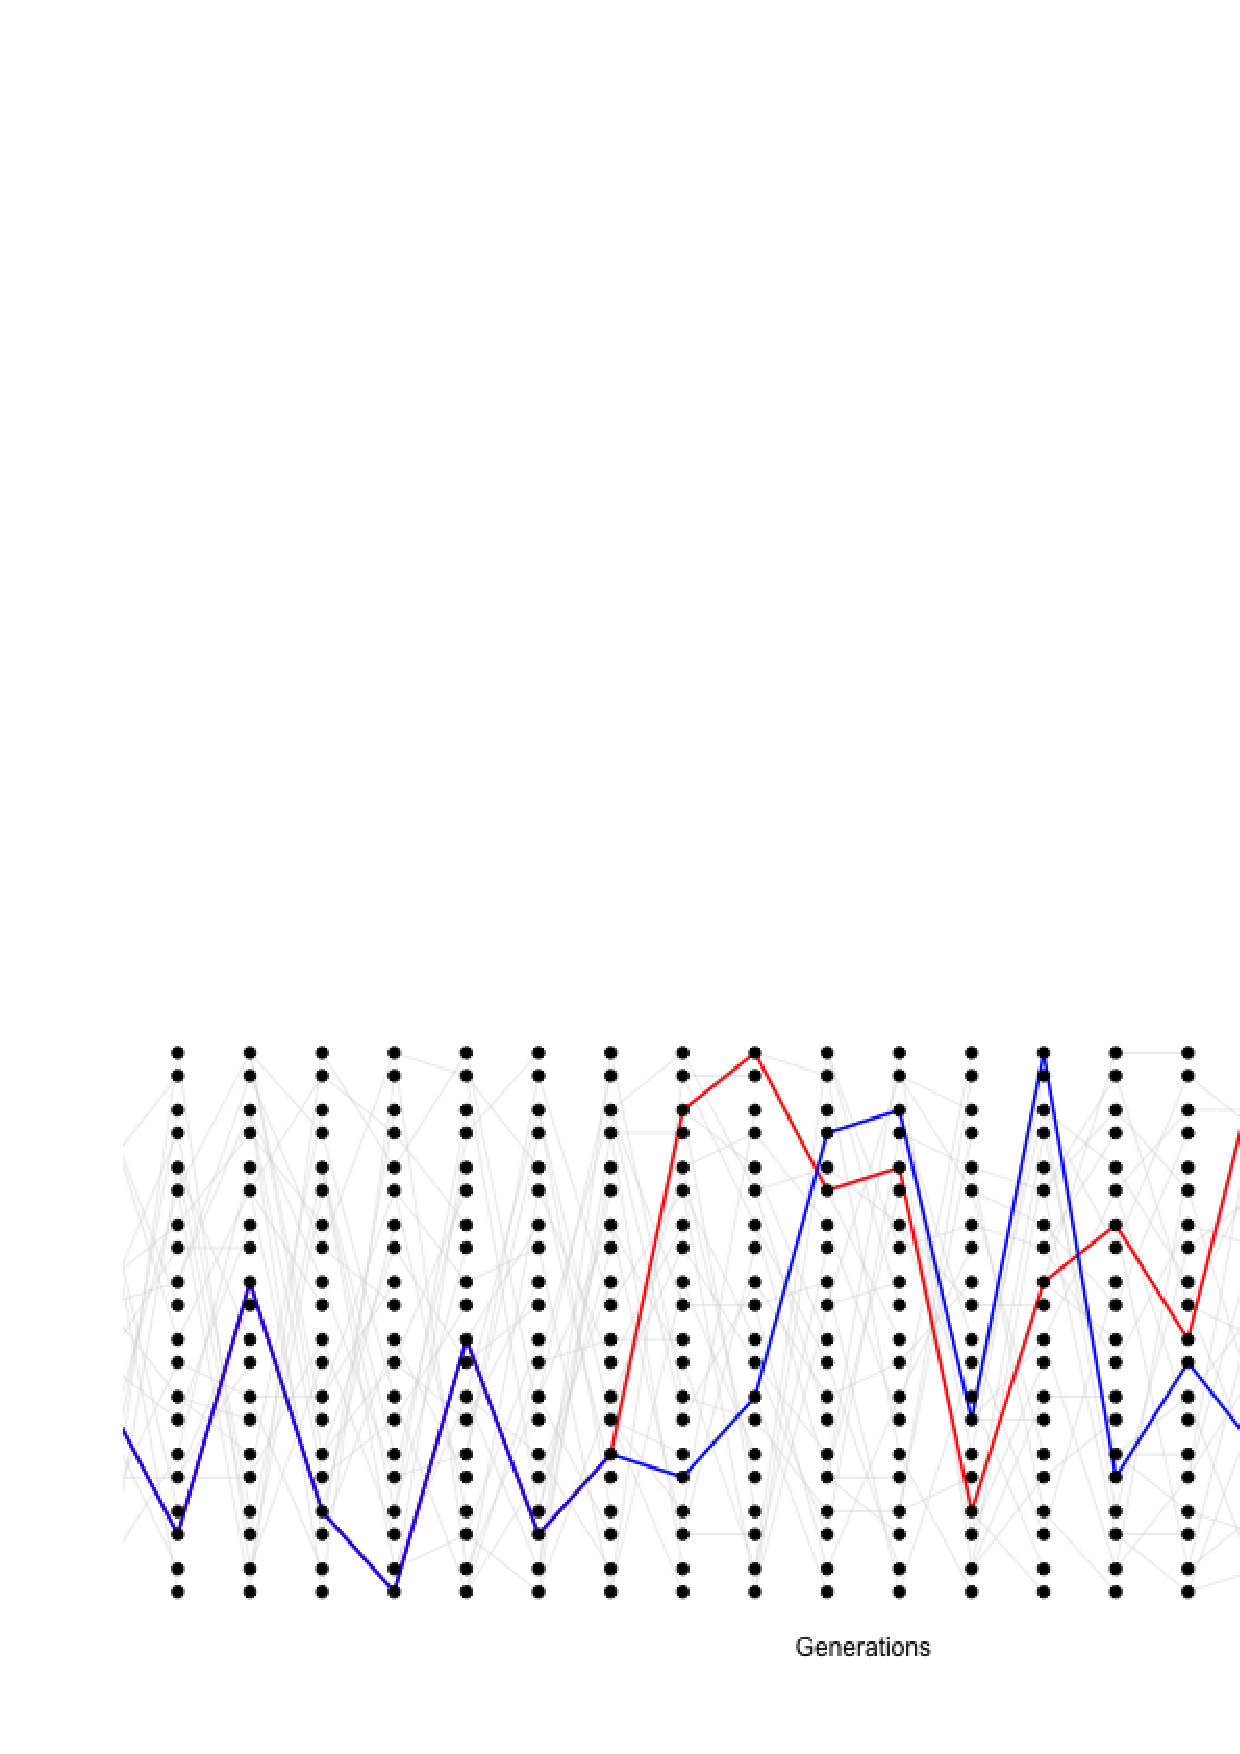
\includegraphics[width=\textwidth]{figures/Coalescent.png}
\end{center}
\caption{A simple simulation of the coalescent process. The simulation
  consists of a diploid population of 10 individuals (20 alleles). In
  each generation, each individual is equally likely to be the parent
  of an offspring (and the allele transmitted is indicated by a light
  grey line).  We track a
  pair of alleles, chosen in the present day, back 14 generations
  untill they find a common ancestor.} \label{fig:Coalescent_simulation}
\end{figure}

\marginnote{Blurring our eyes a little we can see  that \ref{eqn:coal_time_dist} is
\begin{equation}
\approx \frac{1}{2N} e^{-t/(2N)} 
\end{equation}
thus if we wanted a continuous random variable we could say that the coalescent time of a pair of sequences ($T_2$) is
approximately exponentially distributed with a rate $1/(2N)$, i.e. $T_2 \sim \text{Exp}\left( 1/(2N) \right)$. }

\graham{fix equation numbers here}
The probability that a pair of alleles
have failed to coalesce in $t$ generations and then coalesce in the
$t+1$ generation back is
\begin{equation}
  \frac{1}{2N} \left(1- \frac{1}{2N} \right)^{t} \label{eqn:coal_time_dist}
\end{equation}
Thus the coalescent time of our pair of alleles is a Geometrically distributed random variable,
where the probability of success is $1/(2N)$, we've denote this by $T_2 \sim  \text{Geo}(1/(2N))$
The mean coalescent time of a pair of a pair of alleles is $2N$ generations\\

Conditional on a pair of alleles coalescing $t$ generations ago
there are $2t$ generations in which a mutation could occur. If the per
generation mutation rate is $\mu$ then the expected number of
mutations between a pair of alleles coalescing $t$ generations ago is
$2 t\mu$

As our expected coalescent time is $2N$ generations (which follows from the expected value of exponential distributions), the expected
number of mutations separating two alleles drawn at random from the
population is
%
\begin{align}
  \E(j) &= 2\mu\E(t) \\ \nonumber
  &= 4N\mu \\
  &= \theta \nonumber
\end{align}
We'll assume that mutations never happen at the same site twice,
i.e. no multiple hits, such that we get to see all of the mutation events that separate our pair
of sequences \sidenote{This is called the infinitely-many-sites assumption,
which should be fine if $N\mu_{BP} \ll 1$, where $\mu_{BP}$ is the mutation rate per base pair).} Thus the number of
mutations between a pair of sites is the observed number of
differences between a pair of sequences. \\

We'll denote the observed number of pairwise differences at putatively neutral
sites separating a pair of sequences as $\pi$ (we usually average this over a
number of pairs of sequences for a region). So we can estimate of $\theta$ from
$\pi$, $\widehat{\theta}_{\pi}$ by setting $\widehat{\theta}_{\pi}=\pi$.  If we
have an independent estimate of $\mu$, then from setting $\pi =
\widehat{\theta}_{\pi} = 4N\mu$ we can obtain an estimate of the population
size $N$ that is consistent with our levels of neutral polymorphism.

\begin{marginfigure}
\begin{center}
  \includegraphics[width =
  \textwidth]{illustration_images/Quant_gen/Grey_fox/14770789583_4db7ec5164_o.jpg}  %https://www.flickr.com/photos/internetarchivebookimages/14770789583/in/photolist-axdicF-ovfa8V-odM3sY-bCrnQ8-ovgYXn-tiQfMQ-odMpu5-x1xCJu-wQ7qT7-wE7kfs-xEZQd1-wK4YSh-ovWx4g-wpDZzF-xjvQ89-tHDjuS-w9Wit5-xEvyhH-xjCbKD-u4q3Qe
\end{center}
\caption{Gray Fox, {\it Urocyon cinereoargenteiis}. Pearson and Warren. Diseases and enemies of poultry. (1897) BHL.} 
\end{marginfigure}

\marginnote{
\begin{question}
\citet{robinson:16} found that the endangered Californian Channel Island fox on San Nicolas had very
low levels of diversity ($\pi =0.000014 \text{bp}^{-1}$) compared to
its close relative the California mainland gray fox ($0.0012\text{bp}^{-1}$). \\
%\bf A How many sites do you expect to differ between two samples
%sequenced over a 100kb region in each of these populations?\\   
{\bf A)} Assuming a mutation rate of $2\times 10^{-8}$ what
effective population size do you estimate for these two populations?
\\
{\bf B)} Why is the effective population size of the Channel Island fox
so low? [Hint: quickly google Channel island foxes to read up on their
history, also to see how ridiculously cute they are.]
\end{question}
}

\paragraph{More details on the pairwise coalescent.}
\graham{This section is currently where some of the continuous time
  coal. has been moved.}


Conditional on the calescent time $t$ the probability of our pair of alleles are separated by $j$ mutations
since they last shared a common ancestor is
\begin{equation}
P(j | T_2 = t ) = {2t \choose j} \mu^{j} (1-\mu)^{2t-j}
\end{equation}
i.e. mutations happen in $j$ generations, and do not happen in $2t-j$
generations (with ${2t \choose j}$ ways this can possibly
happen). Assuming that $\mu \ll 1$, and that $2t-j \approx 2t$ then we
can approximate the probability that we have $j$ mutations as a
Poisson distribution
\begin{equation}
P(j | T_2 = t ) = \frac{ (2 \mu t )^{j} e^{-2\mu t}}{j!}
\end{equation}
i.e. a Poisson with mean $2\mu t $. \\


\section{The coalescent process of a sample of alleles.}

Usually we are not just interested pairs of alleles, or the
average pairwise diversity, we are interested in the properties of
diversity in samples of a number of alleles drawn from the population.  
To allow for this instead of just following a pair of lineages back until they
coalesce, we can follow the history of a sample of alleles back
through the population.

Consider first sampling three alleles at random from the population. The
probability that all three alleles choose exactly the same ancestral allele one
generation back is $\nicefrac{1}{(2N)^2}$. If $N$ is reasonably large then this
is a very small probability. As such it is very unlikely that our three alleles
coalesce at once, a in a moment we'll see that it is safe to ignore such
unlikely events. \\

\begin{figure}
\begin{center}
  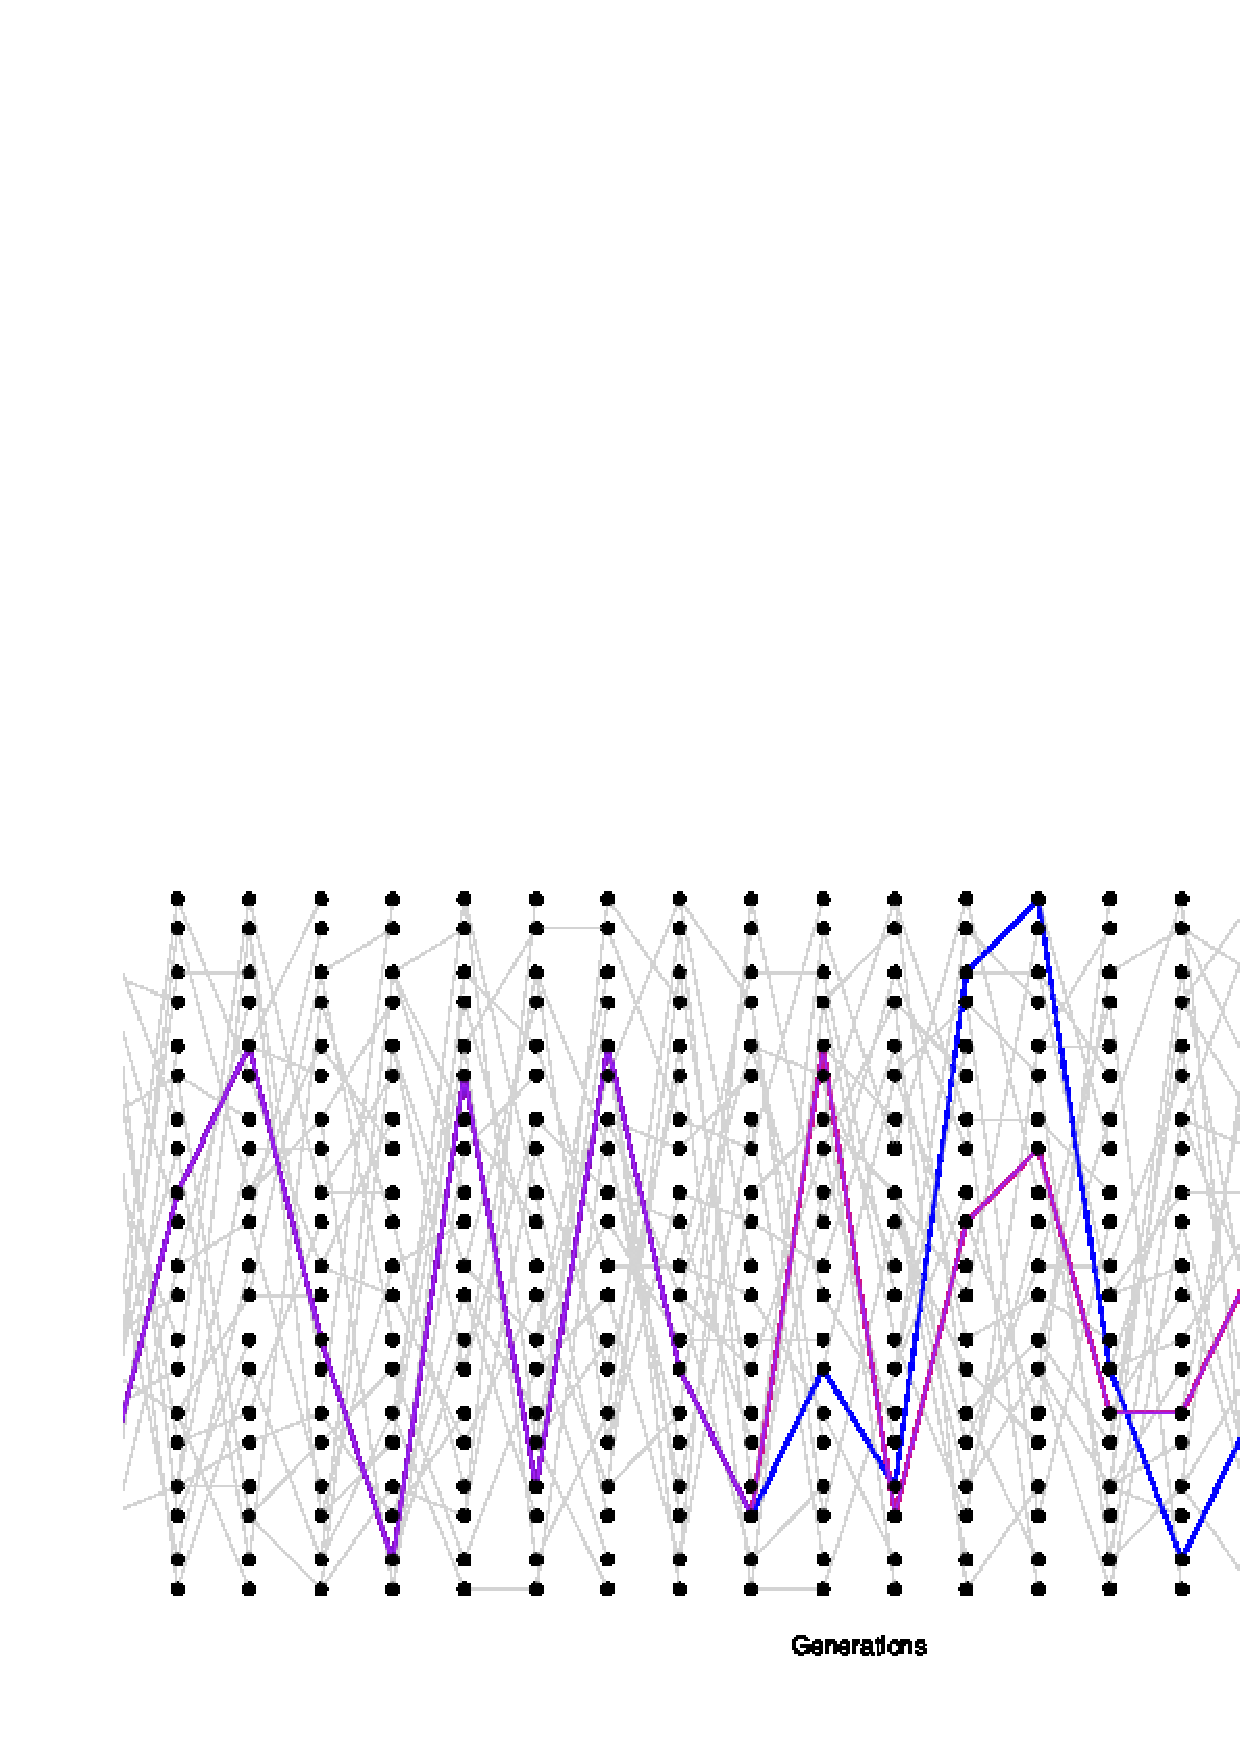
\includegraphics[width = \textwidth]{figures/Coalescent_3.png}
\end{center}
\caption{A simple simulation of the coalescent process for three
  lineages. We track the ancestry of 
  three modern-day alleles, the first pair (blue and purple) coalesce four generations back 
  their are then two independent lineages we are tracking, this pair
  then coalesces twelve generations in the past. Note that different
  random realizations of this process will differ from each other a lot.} \label{fig:Coalescent_simulation_3}
\end{figure}

The probability that a specific pair of alleles find a common ancestor in the
preceding generation is still $\nicefrac{1}{(2N)}$. There are three possible pairs of
alleles so the probability that no pair finds a common ancestor is
\begin{equation}
\left(1-\frac{1}{2N} \right)^3 \approx \left( 1- \frac{3}{2N} \right)
\end{equation}
in making this approximation we are multiplying out the right hand-side
and ignoring terms of $1/N^2$ and higher. See
Figure \ref{fig:Coalescent_simulation_3} for a random realization of this process. \\

More generally when we sample $i$ alleles there are ${i \choose 2}$
pairs,\sidenote{said as ``i choose 2''}  i.e. $i(i-1)/2$ pairs, thus the probability that no pair
of alleles coalesces in the preceding generation is
\begin{equation}
\left(1-\frac{1}{(2N)} \right)^{{i \choose
 2}} \approx \left( 1- \frac{{i \choose
 2}}{2N}\right)
\end{equation}
while the probability of any pair coalescing is $\approx \nicefrac{2N}{{i \choose
 2}}$.\\

We can ignore the possibility of more than pairs of alleles (e.g. tripletons)
simultaneously coalescing at once as terms of $\nicefrac{1}{N^2}$ and higher
can be ignored as they are vanishingly rare. Obviously there are in reasonable
sample sizes there are many more triples (${i \choose 3}$), and higher order
combinations, than pairs (${i \choose 2}$) but if $i \ll N$ then we are safe to
ignore these terms.

\marginnote{
To see the continuous time  version of this note that \eqref{eqn:T_i} is
\begin{equation} 
\approx  \frac{{i \choose
 2}}{2N} \exp \left( - \frac{{i \choose
 2}}{2N} t \right)
\end{equation}
the waiting time $T_i$ to the first coalescent event in a sample
of $i$ alleles is exponentially distributed with rate $\nicefrac{{i \choose
 2}}{2N}$, i.e. $T_i \sim \text{Exp}\left(\nicefrac{{i \choose
 2}}{2N} \right)$. }

When there are $i$ alleles the probability that we wait until the
$t+1$ generation before
any pair of alleles coalesce is
\begin{equation}
 \frac{{i \choose
 2}}{2N}\left( 1- \frac{{i \choose
 2}}{2N}\right)^{t} \label{eqn:T_i}
\end{equation}
thus the waiting time while there are $i$ lineages is a geometrically
distributed random variable with probability of success $ \nicefrac{{i \choose
    2}}{2N}$, which we denote by
\begin{equation}
T_i \sim \text{Geo}
\left(  \nicefrac{{i \choose
      2}}{2N} \right).
\end{equation}
The mean waiting time till any of pair within our
 sample to coalesce is 
\begin{equation}
\E( T_i) \frac{2N}{{i \choose  2}}  \label{eqn:E_T_i}
\end{equation}

When a pair of alleles first find a common ancestral allele some
number of generations back further into the past we only have to keep
track of that common ancestral allele for the pair. Thus when a pair
of alleles in our sample of $i$ alleles coalesce, we then switch to
having to follow $i-1$ alleles back. Then when a pair of these $i-1$
alleles coalesce, we then have to follow $i-2$ alleles back. This
process continues until we coalesce back to a sample of two, and from
there to a single most recent common ancestor (MRCA).\\


\paragraph{Simulating a coalescent genealogy}
To simulate a coalescent genealogy at a locus for a sample of $n$ alleles we therefore simply follow this
algorithm
\begin{enumerate}
\item Set $i=n$.
\item We simulate a random variable to be the time $t_i$ to the next coalescent event from $t_i \sim
  \text{Exp}\left(\nicefrac{{i \choose
 2}}{2N} \right)$
\item Choose a pair of alleles to coalesce at random from all possible
 pairs.
\item Set $i=i-1$
\item Continue looping of steps 1-3 until $i=1$ i.e. the most recent
 common ancestor of the sample is found.
\end{enumerate}
by following this algorithm we are generating realizations of the
genealogy of our sample. \\



\subsection{Expected properties of coalescent genealogies and
  mutations.} 

\begin{figure}
\begin{center}
\includegraphics[width= \textwidth]{figures/Coalescent/Coal_w_muts.pdf}
\end{center}
\caption{ } \label{fig:Coal_w_muts}
\end{figure}


\paragraph{The expected time to the most recent common ancestor.}
We will first consider the time to the most recent common ancestor of
the entire sample ($T_{MRCA}$). This is
\begin{equation}
T_{MRCA} = \sum_{i=n}^2 T_i
\end{equation}
generations back. As our coalescent times for different $i$ are independent, the expected time to the most recent common ancestor
is
\begin{equation}
\E(T_{MRCA}) = \sum_{i=n}^2 \E(T_i) = \sum_{i=n}^2  2N/{i \choose
 2}
\end{equation}
using the fact that $\frac{1}{i(i-1)}=\frac{1}{i-1} - \frac{1}{i}$ with a bit of
rearrangement we can rewrite this is
\begin{equation} 
\E(T_{MRCA}) = 4N\left(1- \frac{1}{n} \right) \label{TMRCA_neutral}
\end{equation}
so the average $T_{MRCA}$ scales linearly with population
size. Interestingly, as we move to larger and larger samples (i.e. $n \gg 1$) the average
time to the most recent common ancestor is converging on $4N$. What's
happening here is that in large samples our lineages typically coalesce rapidly
at the start and very soon coalesce down to a much smaller number of
lineages.   \\


\paragraph{The expected total time in a genealogy and the number of
  segregating sites.}

Mutations fall on lineages of the coalescent genealogy. These mutations affect all
descendants of this lineage, and under the infinitely-many-sites assumption,
create a new segregating site for each new mutation. The mutation process is a
\emph{Poisson process}, and the longer a particular lineage branch, the more
mutations that can accumulate on it. The total number of segregating sites in
the genealogy is thus a function of the \emph{total} amount of time in the
genealogy of the sample, or the sum of all the genealogy branch lengths,
$T_{tot}$. Since our coalescent genealogies are bifurcating (only two lineages
coalesce at once), our total amount of time in the genealogy is:

\begin{equation}
T_{tot} = \sum_{i=n}^2 iT_i
\end{equation}
as when there are $i$ lineages each contributes a time $T_i$ to the
total time. Taking the expectation of the total time in the genealogy
\begin{equation}
\E(T_{tot}) = \sum_{i=n}^2 i \frac{2N}{{i \choose
 2} } = \sum_{i=n}^2 \frac{4N}{i -1} =\sum_{i=n-1}^1 \frac{4N}{i}
\end{equation}
so our expected total amount of time in the genealogy scales linearly
with our population size. Our expected total amount of time is also
increasing with sample size but is doing so very slowly. To see this
more carefully we can see that for large $n$
\begin{equation}
\E(T_{tot}) = \sum_{i=n-1}^1 \frac{4N}{i} \label{eqn:E_T_tot}
\end{equation}
\marginnote{To get a better sense of how this grows with the sample we
  can see that \ref{eqn:E_T_tot} can be approximated by $\int_1^n \frac{1}{i} di
= 4N \log(n-1)$ approximating our sum by an integral, which will work for
large $n$. }
So our expected total amount of time in the genealogy
is growing with $n$ but it is doing so very slowly. This again follows
from the fact that in large samples the initial coalescence usually
happens very rapidly, so that extra samples adds little to the total
amount of time in the tree. \\

We saw above that the number of mutational differences between a pair
of alleles that coalescence $T_2$ generations ago was Poisson with a
mean of $2 \mu T_2$. A mutation that occurs on any branch of our
genealogy will cause a segregating polymorphism in the sample
(making our infinitely-many-sites assumption). Thus if the total time
in the genealogy is $T_{tot}$ there is $T_{tot}$
generations for mutations. So the total number of mutations
segregating in our sample ($S$) is Poisson with mean $\mu T_{tot}$. Thus the
expected number of segregating in history a sample of size $n$ is
\begin{equation}
\E(S) = \mu \E(T_{tot}) = \sum_{i=n-1}^1 \frac{4N\mu }{i} = \theta
\sum_{i=n-1}^1 \frac{1}{i}
\end{equation}
Thus we can use this formula to derive another estimate of the
population scaled mutation rate, by setting our observed number of
segregating sites in a sample ($S$) equal to this expectation. We'll call this estimator $\widehat{\theta}_W$
\begin{equation}
\widehat{\theta}_W =\frac{ S}{\sum_{i=n-1}^1 \frac{1}{i}}   \label{watterson_theta}
\end{equation}
this estimator was devised by \citeauthor{watterson:75}, hence the $W$.


\paragraph{The neutral site-frequency spectrum.}

We can use our coalescent process to find our the expected number of
alleles present $i$ times out of $n$, e.g. how many singletons do we
expect to find in our sample?  

\begin{marginfigure}
\begin{center}
\includegraphics[width= \textwidth]{figures/Genetic_drift/freq_spec_tree.pdf}
\end{center}
\caption{A tree for three samples, note that this is the only possible
tree shape (treating the tips as unlabelled)} \label{fig:freq_coal}
\end{marginfigure}

To see how we could go about working this out, lets start by
considering the coalescent tree, shown in \ref{fig:freq_coal}, for sample of $3$ alleles drawn from a
population. Mutations that fall on the
branches coloured in black will be derived singletons, while mutations that
fall along the orange branch will be doubletons in the sample. The
total number of generations where a singleton mutation could arise is
$3 T_3 + T_2$, note that we only count the time where there are two
lineages once. While the time where doubletons could arise is
$T_2$. So our expected number of singletons, using eqn \eqref{eqn:E_T_i}, is 
\begin{equation}
\E(S_i) = \mu \left( 3\E(T_3) +  \E(T_3) \right) = \mu \left( 3
  \frac{2N}{3}+ 2N \right) = \theta
\end{equation}
by similar logic our expected number of doubletons is $\E(S_i)
=\theta/2$, i.e. there are half as many doubletons as singletons. 

Extending this logic to large samples is doable, but tedious
\graham{Give  numbers for 10 tips}. A nice
simple proof of the neutral site frequency spectrum is given by
\citeauthor{Hudson:15}, but we won't give this here. The general form is: 
\begin{equation}
\E(S_i) = \theta \frac{1}{i}   \label{eqn:neutral_freq_spec}
\end{equation}
there are twice as many singletons as doubletons, three times as many
singletons as tripletons, and so on. The other thing that will be
helpful for us to know is that neutral alleles at intermediate frequency tend to be old, and
those that are rare in the sample are young.

\begin{question}
There are two possible tree shapes that could relate four
samples. Colour (or otherwise mark) the branches by where singletons,
doubletons, and tripleton derived alleles could arise. 

Can you work out the expected number of each types of allele?
\end{question}


\paragraph{tests based on the site frequency spectrum}
A variety of tests of whether site frequency spectrum conforms to its
neutral, constant-population expectations have been proposed. This is
useful for detecting population size changes using many loci data, or
for detecting the signal of selection at individual loci. One of
the first was proposed by \citeauthor{tajima:89}, and is called
Tajima's $D$. Tajima's $D$ is
\begin{equation}
  D = \frac{\theta_{\pi}-\theta_{W}}{C} \label{eqn_Tajimas_D}
\end{equation}
where the numerator is the difference between the estimate of
$\theta$ based on pairwise differences and that based on segregating
sites. As these two estimators both have expectation $\theta$ under
the neutral, constant-population model the expectation of $D$ is zero. The denominator $C$ is the square-root of an estimator
variance of this difference, the idea being for $D$ to have mean zero
and variance $1$. \\

An excess of rare alleles compared to the constant-population, neutral
model will result in the negative Tajima's $D$, because each
additional rare allele increases the number of segregating sites by
$1$, but only has a small effect on the pairwise differences. 
A positive Tajima's $D$ reflects an excess of intermediate frequency alleles, relative to
the  constant-population, neutral model. As intermediate-frequency, neutral alleles increase pairwise diversity
more per segregating site than a typical neutral alleles.


\subsection{Demography and the coalescent}

\begin{marginfigure}
\begin{center}
  \includegraphics[width = \textwidth]{Journal_figs/genetic_drift/human_pop_growth/Nelson_pop_growth.pdf}
\end{center}
\caption{Data from 202 genes from 14002 people of European ancestry (28004 alleles). Note
  the double log-scale. Redrawn from \citeauthor{nelson:12}. The red
  line gives the neutral, constant population size estimate using a
  $\theta$ estimated from $\pi$.} \label{fig:Human_growth}
\end{marginfigure}
We've already seen how changes in population size can change the rate
at which heterozygosity is lost from the population (see the
discussion around eqn. \eqref{eqn:var_pop_coal}). If the population
size in generation $i$ is $N_i$ the probability that a pair of
lineages coalesce is $\nicefrac{1}{2N_i}$, this conforms to our
intuition that if the population size is small that the rate at which
pairs of lineages find their common ancestor is faster. If the
population randomly fluctuates rapidly in size throughout 
we can often accomodate this simply by using the effective popuation size $N_e$ in place of $N$. However,
longer term more systematic changes in population size will distort
the coalescent genealogies, and hence patterns of diversity, in more
systematic ways. 

As an example of how demography can potentially distort patterns left
in a sample the observed frequency spectrum from a very large sample of humans, shown in Figure \ref{fig:Human_growth}. For
comparison the neutral frequency spectrum, eqn
\eqref{eqn:neutral_freq_spec}, is shown as a red line. There are
  vastly more rare alleles than expected under our neutral, constant-population-size model. 

\begin{figure}
\begin{center}
  \includegraphics[width = \textwidth]{figures/Genetic_drift/Demography/Growth_genealogy.pdf}
\end{center}
\caption{} \label{fig:Genealogy_growth}
\end{figure}

Why is this? Well this is likely the result of the very recent
explosive growth in human populations. If the population has grown rapidly then the pairwise-coalescent
rate in the past may be much higher than closer to the present. (see Figure \ref{fig:Genealogy_growth}). 

The first consequence of this is that they'll be much less genetic
diversity in the population than you'd predict using the census
population size. One example of this is in humans, there's $7$ billion
of us alive today, but this is due to very rapid population growth
over the past thousand to tens of thousands of years. Our level of
genetic diversity is very much lower than you'd predict given our
census size. The second consequence is that the deeper coalescent branches are
much more squished together in time, compared to those in a constant
population.  These deeper branches are the source of alleles at more
intermediate frequency, and so there are even fewer of these alleles
in growing populations. That's why there are so many rare alleles,
especially singletons in this large sample of Europeans. 


Another common demographic scenerio is a population population
neck. Here the population size crashes dramatically, and subsequently
recovers. For example our population may have size $N_{\textrm{Big}}$
and have crashed down to $N_{\textrm{Small}}$, one example of a
bottleneck is shown in Figure \ref{fig:Genealogy_crash}. 
\begin{figure}
\begin{center}
  \includegraphics[width = \textwidth]{figures/Genetic_drift/Demography/Crash_genealogy.pdf}
\end{center}
\caption{} \label{fig:Genealogy_crash}
\end{figure}
Looking at a sample of lineages drawn from the population today, if
the bottleneck was somewhat recent, $\ll N_{\textrm{Big}}$ generations
in the past, many of our lineages will not have coalesced by the time
the bottleneck moving backward in time. But during the bottleneck our
lineages coalesce at a much higher rate, such that many of our
lineages will coalesce if the bottneck lasts long enough
($\sim N_{\textrm{Small}}$ generations). If the bottleneck is very
strong then all of our lineages will coalesce during it, and this may
look very like our population growth model (with an excess of rare
alleles). However, if some pairs of lineages escape coalescing during
the bottleneck they will coalesce much more deeply in time (e.g. the
blue and orange ancestral lineages in
\ref{fig:Genealogy_crash}). 
\begin{figure}
\begin{center}
  \includegraphics[width = \textwidth]{figures/Genetic_drift/Demography/Mimulus_coalescent_times.pdf}
\end{center}
\caption{Black dots give $\pi$ in 1kb windows, the red line is a
  moving average (data from  \citeauthor{brandvain:14}). Pairwise coalescent times ($t$) estimated assuming $\pi = 2 t
  \mu$m using $\mu_{BP}=10^{-9}$.} \label{fig:Mimulus_bottleneck}
\end{figure}
An example of this is shown Figure
\ref{fig:Mimulus_bottleneck}, data from \citeauthor{brandvain:14}. {\it Mimulus nasutus} is a selfing
species that arose recently from out-crossing progenitor {\it M.
  guttatus}, and experienced a strong bottleneck. {\it M. guttatus} has a very high levels of genetic diversity
($\pi=4\%$ at synonymous sites), but {\it M. nasutus} has lost much 
of this diversity ($\pi =1\%$). Looking along the genome, between a
pait of {\it M. guttatus} chromosomes, levels of
diversity are fairly uniformly high.
\begin{marginfigure}
\begin{center}
  \includegraphics[width = 0.75 \textwidth]{illustration_images/Genetic_drift/Mimulus/Mimulus.png}
\end{center}
\caption{{\it M. guttatus} by Pierre-Joseph
  Redout\'e.} \label{fig:Human_growth}  %é
\end{marginfigure}
 But in comparing two {\it
  M. nasutus} diversity is low because the pair of lineages coalesce
recently; in a few places we see levels of diversity comparable to
{\it M. guttatus}, these regions correspond to our pair of lineages
failing to coalesce during the bottleneck and subsequently coalescing
much more deeply in the ancestral {\it M. guttatus} population.


Mutations that arise on these deeper lineages will be at intermediate frequency in our sample, and so mild bottlenecks
can lead to an excess of intermediate frequency alleles compared to
the standard constant-population model. This can result in skew 
Tajima's D, see eqn \ref{eqn_Tajimas_D}, towards positive values and away from its expectation of
zero . One example of this skew is shown in Figure
\ref{fig:maize_Tajimas_D}. Maize ({\it Zea mays}) was domesticated
  from its wild progenitor teosinte ({\it Z. }) roughly ten thousand years ago. We can see how the
 bottleneck associated with domestication as resulted in a loss of
 genetic diversity in maize and a skew
 towards intermediate frequency polymorphisms and so more positive
 values of Tajima's D.


\begin{figure}
\begin{center}
  \includegraphics[width = \textwidth]{Journal_figs/genetic_drift/Maize_bottleneck/Wright_Tajima_D.pdf}
\end{center}
\caption{Data for polymorphism from Maize and Teosinite 774
  genes redrawn from \citeauthor{Wright:05}{\bf Left)} Genetic
  diversity levels in maize and and Teosinte at each of these genes.
Note how diversity levels are lower in maize than teosinte, i.e. most
points are below the red $x=y$ line.  
. {\bf Right)}The distribution of Tajima's D in maize and teosinte. } \label{fig:maize_Tajimas_D}  %é
\end{figure}

\begin{marginfigure}
\begin{center}
  \includegraphics[width = \textwidth]{illustration_images/Genetic_drift/maize/7845339168_66aa3d8ccc_z.jpg}
\end{center}
\caption{Maize ({\it Zea mays}.) Prof. Dr. Thomé's Flora von
  Deutschland. 1886. Thomé, O. W. } \label{fig:maize}  %é
\end{marginfigure}



\section{Molecular Evolution and the fixation of neutral alleles} 
It is very unlikely that a rare
neutral allele accidentally drifts up to fixation; more likely, such an allele
will be eventually lost from the population. However, populations experience a
large and constant influx of rare alleles due to mutation, so even if it is
very unlikely that an individual allele fixes within the population, some
neutral alleles will fix by chance.  \\


%We'll first consider the probability that a neutral allele fixes
%within the population, starting from it just enters a diploid
%population as a newly mutated allele at frequency $1/(2N)$.

%so for an allele to be fixed in the population it
%must have been that allele

\paragraph{Probability of the eventual fixation of a neutral allele}
% TODO: tried to clean up this section, needs more work
An allele which reaches fixation within a population is an ancestor to the
entire population. In a particular generation there can be only single allele
that all other alleles at the locus in later generation can claim as an
ancestor. A neutral locus, the actual allele does not affect the number of
descendents that the allele has (this follows from the definition of
neutrality: neutral alleles don't leave more or less descendents on average).
An equivalent way to state this is that the allele labels don't affect
anything; thus the alleles are \emph{exchangeable}. As a consequence of this,
any allele is equally likely to be the ancestor of the entire population.  In a
diploid population size of size $N$, there are $2N$ alleles all of which are
equally likely to be the ancestor of the entire population at some later time
point. So if our allele is present in a single copy, the chance that it is the
ancestor to the entire population in some future generation is
$\nicefrac{1}{(2N)}$, i.e. the chance our neutral allele is eventually fixed is
$\nicefrac{1}{(2N)}$.  See Figure \ref{fig:subs_simulation}, our orange allele
in the first generation is one of 10 differently coloured alleles, and so has a
$1/10$ chance of being the ancestor of the entire population at some later time
point (as it is by the 9th generation).\\

More generally if our neutral allele is present in $i$ copies in the
population, of $2N$ alleles, the probability that this allele is fixed is
$\nicefrac{i}{(2N)}$, i.e. the probability that a neutral allele is eventually
fixed is simply given by its frequency ($p$) in the population.  (We can also
derive this result by letting $Ns \rightarrow 0$ in eqn.
\eqref{eqn:prob_fixed}, a result we'll encounter later.)

\begin{figure}
\begin{center}
  \includegraphics[width = \textwidth]{figures/Substitution_sim.png}
\end{center}
\caption{Each allele initially present in a small diploid population is
  given a different colour so we can track their descendants over
  time. By the 9th generation all of the alleles present in the
  population can trace their ancestry back to the orange allele.} \label{fig:subs_simulation}
\end{figure}


% TODO
An allele newly arisen mutation only becomes a fixed difference if it is lucky
enough to be the ancestor of the entire population. As we saw above this occurs
with probability $\nicefrac{1}{(2N)}$. How long does is take on average for
such an allele to fix within our population? Well in developing
equation \eqref{TMRCA_neutral} we've seen that it takes $4N$
generations for a large sample of alleles to all trace their ancestry back to a
single most recent common ancestor. Thus it must take roughly $4N$ generations
for a neutral allele present in a single copy within the population to the
ancestor of all alleles within our population. This argument can be made more
precise, but in general we would still find that it takes $\approx 4N$
generations for a neutral allele to go from its introduction to fixation with
the population.   \\

\paragraph{Rate of substitution of neutral alleles}

A substitution between populations that do not exchange gene flow is simply a
fixation event within one population. The rate of substitution is therefore the
rate at which new alleles fix in the population, so that the long-term
substitution rate is the rate at which mutations arise that will eventually
become fixed within our population.\\

Assume that there are two classes of mutational changes that can occur with a
region, highly deleterious mutations and neutral mutations. A fraction $C$ of
all mutational changes are highly deleterious, and can not possibly contribute
to substitution nor polymorphism (i.e. $Ns \gg 1$).  The other $1-C$ fraction
of mutations are neutral. If our mutation rate is $\mu$ per transmitted allele
per generation, then a total of $2N \mu (1-C)$ neutral mutations enter our
population each generation.\\

Each of these neutral mutations has a $\nicefrac{1}{(2N)}$ probability chance of
eventually becoming fixed in the population. Therefore, the rate at
which neutral mutations arise that eventually become fixed within our
population is  
\begin{equation}
2N\mu(1-C)\frac{1}{2N} = \mu(1-C)
\end{equation}
thus the rate of substitution under a model where newly arising alleles are either
highly deleterious or neutral, is simply given by the mutation rate
towards neutral alleles, i.e. $\mu(1-C)$.\\

Consider a pair of species have diverged for $T$ generations, i.e. orthologous sequences shared between the species last shared a common ancestor $T$ generations ago. If they have maintained a constant $\mu$ over that time, will have accumulated an average of
\begin{equation}
2\mu(1-C)T
\end{equation}
neutral substitutions. This assumes that $T$ is a lot longer than the time it
takes to fix a neutral allele, such that the total number of 
alleles introduced into the population that will eventually fix is the
total number of substitutions. We'll see below that a neutral allele
takes on average $4N$ generations to fix from its introduction into
the population.\\

This is a really pretty result as the population size has completely canceled
out of the neutral substitution rate. However, there is another way to see this
in a more straight forward way. If I look at a sequence in me compared to say a
particular chimp, I'm looking at the mutations that have occurred in both of
our germlines since they parted ways $T$ generations ago. Since neutral alleles
do not alter the probability of their transmission to the next generation, we
are simply looking at the mutations that have occurred in $2T$ generations
worth of transmissions. Thus the average number of neutral mutational
differences separating our pair of species is simply $2\mu (1-C) T$.\\

\begin{marginfigure}
\begin{center}
\includegraphics[width=0.8 \textwidth]{figures/Genetic_drift/ILS/split_anc_pop.pdf}
\end{center}
\caption{} \label{fig:split_anc_pop}  
\end{marginfigure} 


If we are considering $T$ to represent the divergence between long
separated species, then we can think of $T$ as the time that the
species split. However, for more recently diverged populations and
species, we need to include the fact that the sorting of ancestral
polymorphism contributes to divergence among species. In Figure 
\ref{fig:split_anc_pop}, we see a lineage selected from population A
and B, with three mutations that separate them shown as dashes. Our two populations split $T_s$ generations ago.  However, the
coalescence of our A and B lineage is necessarily deeper in time than
$T_s$. The top mutation was polymorphic in the ancestral population
but now contributes to the divergence between A and B. Assuming that
our ancestral population had effective size of $N_A$ individuals, and
that our populations split cleanly with no subsequent gene flow, then
\begin{equation}
T = T_s + 2N_A.
\end{equation}
Therefore, polymorphism in the ancestral population can make up a
sizable proportion of the divergence between closely related
species/populations. \graham{lineup split time in this section w. FST section.}



\begin{question}
For this, and the next question, assume that humans and chimp diverged
\graham{Update numbers?}
around 5.5$\times 10^6$ years, a generation time ~20 years, that the speciation occurred instantaneously in allopatry with no subsequent gene flow, and the ancestral effective population size of the human and chimp common ancestor population was 10,000 individuals.\\
Nachman and Crowell sequenced 12 pseudogenes in human and chimp found substitutions at 1.3\% of sites. \\
{\bf A) } What is the mutation rate per site per generation at these genes?\\
{\bf B)} All of the pseudogenes they sequenced are on the autosomes. What
would you prediction be for pseudogenes on the X and Y chromosomes,
given that there are fewer rounds of replication in the female
germline than in the male germline.
\end{question}

\section{Tests of molecular evolution.}

\subsection{Comparing the rates of non-synonymous to synonymous
substitutions $\dNdS$}
A common test molecular evolution is to compare the ratio of the rates of non-synonymous to synonymous
substitutions. The simplest way to calculate $d_N$ is to 
count up the non-synonymous changes and divide by the total number of
positions in the gene where a non-synonymous change could occur. We
can do likewise for $d_S$, and then take the ratio. This is a helpful
conceptual way to think about what $\dNdS$ represents, however, this
ignores the fact that particular changes are more likely to occur by
mutation and also does not account for multiple hits. Therefore, in
practice $\dNdS$ is more usually calculated by model-based
likelihood and bayesian methods
that can account for these features (see \gc{XX}). 

For the vast majority of genes in the genome we see that $\dNdS < 1$, this is consistent with the view
that non-synonymous sites are much more constained than synonymous,
i.e. that most non-synonymous mutations are deleterious and quicky
removed from the population. If we are willing to make the assumption that all synymous changes are
neutral, $d_S=2T \mu$, then we can estimate the degree of constraint. (Note that synonymous changes can sometimes be subject to
both positive and negative selection, but we have to start somewhere.) 

Assuming that a fraction $C$ of non-synonymous changes are too
deleterious to contribute to polymorphism then, if $T$ generations of divergence have
elapsed between the two populations we expect
\begin{equation}
d_N = 2T (1-C) \mu  
\end{equation}
Then
\begin{equation} 
\dNdS = (1-C) 
\end{equation}
therefore, if we assume that non-synonymous mutations can only be
strongly deleterious or neutral, we estimate the fraction of mutational changes that
are constrained by negative selection as $C= 1- \dNdS$. This has the
interpretations of being the fraction of non-synonymous mutations that
are quickly weeded out of the populaiton by selection, and so do not
contribute to divergence among species. 

\paragraph{Loss of constraint at pseudogenes.}

\begin{marginfigure}
\begin{center}
\includegraphics[width=\textwidth]{illustration_images/Genetic_drift/sloth/20423856040_6e4360df9c_z.jpg}
\end{center}
\caption{Two-toed sloth ({\it Choloepus hoffmanni}). An introduction
  to the study of mammals, living and extinct. 1891. Flower W. H. and Lydekker R.} \label{fig:sloth}  
\end{marginfigure} 

While most genes evolve under constraint, we can find examples of
genes that are evolving in a less constrained manner. The simplest
example of this is where the gene has lost function, e.g. has recently
become pseudogenized. When a gene completely loses function there will be no
selection against non-synoynous changes and so they are just as free
to accumulate as synonymous changes, and so $\dNdS=1$.
Genes can lose function because of inactivating mutations that stop
them being transcribed or translated into functional proteins, such genes are
called pseudogenes. Our genomes are filled with old pseudogenes whose
meaning are slowly being eroded through the accumulation of neutral substitutions.
One nice example of as gene that has been repeatedly lost function,
i.e. become repeatedly psuedogenized, is
the Enamlin gene from the study of \citeauthor{Meredith:09}.

\begin{figure}
\begin{center}
\includegraphics[width=\textwidth]{Journal_figs/genetic_drift/Enamelin/Enamlin.pdf}
\end{center}
\caption{Examples of frameshift mutations (insertions blue, deleteions
  red) and premature stop codons in Enamlin in Cetacea and
  Xenarthra. Figure taken from \citeauthor{Meredith:09}} \label{fig:Enamlin_coding}  
\end{figure} 

\marginnote{
``Rudimentary organs may be compared with the letters in a word, still
retained in the spelling, but become useless in the pronunciation, but
which serve as a clue .. for its derivation.'' 
}  %http://darwin-online.org.uk/Variorum/1859/1859-456-dns.html
\graham{get Darwin page number etc}

The protein Enamlin is a key structural protein involved in the outer cap of enamel on teeth. Various mammals have
secondarily evolved to lack enamel on their teeth, because their diet does not
demand hard teeth, e.g. : two-toed sloths ({\it Choloepus}); Pygmy sperm whales ({\it Kogia}); aardvark 
{\it Orycteropus}). While others have lost their teeth entirely: giant anteaters ({\it Myrmecophaga}); Baleen whales, including 
or lack enamel on their teeth.
Due to this loss of selective function
pseudogenizing substitutions, premature stop codons and frameshift mutations, have
accumulated in the gene Enamlin (see Figure \ref{fig:Enamlin_coding}
for examples).  \citeauthor{Meredith:09} sequenced Enamlin across a
range of species and found that none of the species with Enamel have frameshift
mutations in Enamlin, while 17/20 of species that lack Enamel or teeth have
frameshifts in Enamlin and all of them carry premature stop codons
(Figure \ref{fig:Enamlin_phylo}). 

\begin{figure}
\begin{center}
\includegraphics[width=0.8 \textwidth]{Journal_figs/genetic_drift/Enamelin/Enamlin_phylo.pdf}
\end{center}
\caption{The tooth symbol next to each taxon shows whether they have
  teeth, lack enamel, or lack teeth. Branches of the phylogeny are coloured by whether their
  Enamlin is functional (black), pre-mutation (blue), mixed (purple),
  and pseudogenic (red). The black and white vertical bars on branches show frameshift
  mutations.  The Numbers after taxon names indicate minimum number of
  stop codons in the sequence /  the length of the sequence.} \label{fig:Enamlin_phylo}  
\end{figure} 

The branches of the Enamlin phylogeny with a functional Enamlin gene (black)
had an estimated $\dNdS= 0.51$ consistent with the protein evolving in
a constrained manner. While the branches with a pseudogenized Enamlin
had $\dNdS = 1.02$ consistent with the gene evolving an unconstrained
way. The branches where the gene was likely transitioning from a functional
to non-function state (premutation and mixed, blue and purple) had an intermediate values of
$\dNdS=0.83-0.98$ consistent with them transitioning from a
constrained to unconstrained mode of protein evolution.

%\begin{question}
%Enamlin was pseudogenized somewhere along the branch leading to
%Aardvarks ({\it Orycteropus}). This branch has $\dNdS=0.75$
% https://journals.plos.org/plosgenetics/article?id=10.1371/journal.pgen.1000634#pgen.1000634.s007
%dawn pangloin
%https://commons.wikimedia.org/wiki/File:Eomanis_waldi_4.jpg
%% aadvark https://www.flickr.com/photos/internetarchivebookimages/20514695666/in/photolist-xfPbiq-xUcng7-xCyGQA-xdRRQ3-wPMGZr-tFgYfN-wPMPkT-tDahHQ-xuc4KM-xKR4u3-xUkupQ-w88zeU-xMia2r-sp4Aq5-x1wNyZ-xMi46D-tDaCr7-sJE2X4-tFB8Lc-wHWiNj-tp8AUk-tFvh4R-xu3M7w-toUVwN-wYWgVi-w34vHn-x9xAfL-wWhnso-ovvmHE-tG5AgB-xdUzWD-y82dEG-xCA7kx-xV5xWg-wYc33H-wYbFdX-wYbBMP-xUcjpL-xKQjHw-xJmBQU-xKPwEQ-xLEzv4-xu3wHJ-xLEg9V-xnA6Lr-x684wQ-wZNgpq-wYcVbh-wZtb3F-wYbJLh
%%% w1 t/T + w2(T-t)/T = wT
%% https://journals.plos.org/plosgenetics/article?id=10.1371/journal.pgen.1000634#pgen.1000634.s007



%\end{question}
\paragraph{Adaptive evolution and $\dNdS$.}
Clearly genes are not only subject to neutral and deleterious
mutations, beneficial mutations must also arise and fix from from time to time. 
Lets assume that a fraction $B$ of non-synonymous mutations that arise are
beneficial, and that they fix with probability $f_B$. This fixation
probability may be much higher than that of neutral mutations (we'll
discuss how to calculate the fixation probability for beneficial
alleles in Chapter \ref{Selection_Stochasticity}).  If $T$ generations of divergence have
elapsed between the two populations 
\begin{equation}
2T (1-C - B) \mu  + 2T B f_B \mu
\end{equation}
Then
\begin{equation} 
\dNdS = (1-C-B) +  B f_B
\end{equation}
Note that this means that our estimates of $C$ using $1-\dNdS$ will be
a  lower bound on the true constraint if even a small fraction of
mutations are beneficial.
However, genes may still evolve in a constrained way
(i.e. $\dNdS<1$)  if adaptive substitutions are common at a gene if
they are outweighed by the loss of potential subsitutions to negative selection.

While most genes evolve under constraint, we can find examples of
genes that are evolving in a less constrained manner. The simplest
example of this is where the gene has lost function, e.g. has recently
become pseudogenized. Along branches of the phylogeny where all the
constraint against non-synonymous mutation has
been lost then $\dNdS=1$. We can also identify cases where the gene
is evolving more rapidly at the protein level than at synonymous
sites, i.e. $d_N/d_S > 1$, corresponding to cases of rapid change due
to positive selection. 

\begin{figure}
\begin{center}
\includegraphics[width=0.8 \textwidth]{Journal_figs/genetic_drift/Yang_lysozyme/Yang_lysozyme.pdf}
\end{center}
\caption{A phylogram for the primate lysozyme gene redrawn from
  \citeauthor{Yang:98}. For each branch the numbers give the estimated average
number of non-synonymous to synonymous changes in the lysozyme protein.} \label{fig:lysozyme}  
\end{figure} 

\begin{marginfigure}
\begin{center}
\includegraphics[width=0.8 \textwidth]{illustration_images/Genetic_drift/Colobus/19792029373_fcce706e67_k.jpg}
\end{center}
\caption{Abyssinian black-and-white colobus ({\it Colobus guereza}). Brehm's Tierleben,  Brehm,
  A.E. 1893. A member of the leaf-eating Colobines.} \label{fig:Colobus}  
\end{marginfigure} 

\begin{marginfigure}
\begin{center}
\includegraphics[width=0.8  \textwidth]{illustration_images/Genetic_drift/Hoatzin/14747388314_85798ba97e_z.jpg}
\end{center}
\caption{ (hoatzin ({\it Opisthocomus hoazin}). A history of birds
  Pycraft, W.P. 1910.  A leaf-eating bird.} \label{fig:hoatzin}  
\end{marginfigure} 
A classic example of looking for adaptive evolution using dN/dS is the
evolution of the lysozyme protein in primates \citep{Messier:97,Yang:98}, see
the phylogeny in Figure \ref{fig:lysozyme}. The lysozyme protein is
a key component for the breakdown of bacterial walls. It shows very
fast protein evolution notably on the lineages leading to apes (e.g. gibbons
and humans) and Colobines (e.g. colobus and langur monkeys). Colobines have leaf-based diets. They digest
these leaves by fermentation with bacteria in their foregut, and use lysozymes to break down the bacteria to extract energy from the
leaves. In Colobines the lysozyme protein has evolved to work well in the high-PH environment of the stomach. Remarkably the Colobine
lysozyme has convergently evolved this activity via very similar
amino-acid changes at 5 key residuals as in cows and Hoatzins (a leaf
eating bird). 

\paragraph{The Mcdonald-Kreitman test}
\citet{mcdonald:91} devised a simple test of the neutral theory of molecular
evolution at a gene (building on the conceptually similar HKA
test\cite{HKA}. They partitioned polymorphism and fixed differences into 
nonsynonymous and synonymous changes:
\begin{center}
%\begin{table}
\begin{tabular}{ccc}
 & Poly. & Fixed \\
\hline 
Non-Syn. &    $P_N$  &   $D_N$  \\
Syn. &    $P_S$   &     $D_S$   \\
Ratio & $P_N/P_S$ & $D_N/D_S$
\end{tabular}
\end{center}

Under neutral theory we expect a smaller number of non-synonymous to
synonymous fixed differences ($P_N/P_S < 1$) but exactly the same
expectation holds for polymorphism
($P_N/P_S$). To see this denote the total time on the coalescent genealogy within the species as
$T_{tot}$ and the total time for fixed differences by $T_{div}'$ then:

\begin{marginfigure}
\begin{center}
\includegraphics[width=0.8 \textwidth]{figures/Coalescent/MK_tree.pdf}
\end{center}
\caption{ } \label{fig:MK_tree}
\end{marginfigure}

\begin{center}
\begin{tabular}{ccc}
 & Poly. & Fixed  \\
 \hline
Non-Syn. &    $\mu_N T_{tot}$  &   $\mu_N  T_{div}'$ \\
Syn. &    $\mu_S T_{tot}$   &     $\mu_S  T_{div}'$  \\
Ratio & $\mu_N/\mu_S$  & $\mu_N/\mu_S$
\end{tabular}
\end{center}
Therefore, we expect the ratio of non-synonymous to synonymous changes
to be the same for polymorphism and divergence. We can test this expectation of equal ratios via the standard G-test of a $2
\times 2$ table.

\subsection{Neutral diversity and population structure}
%%this section was moved from the coalescent chapter
Up to now we have assumed that our alleles that we have modelled in the
coalescent setting are drawn from a randomly mating population such
that any pair of lineages is equally likely to coalesce with each
other. However, when there is population structure this assumption is
violated. \\

We have previously written the measure of population structure
$\fst$ as
\begin{equation}
\fst = \frac{H_T-H_S}{H_T}
\end{equation}
where $H_S$ is the probability that two alleles sampled at random from a
subpopulation differ, and $H_T$ is the probability that two alleles
sampled at random from the total population differ. 

\paragraph{A simple population split model}
Imagine a population of constant size of $N_e$ diploid individuals that
$\tau$ generations in the past split into two daughter populations (sub-populations)
each of size $N_e$ individuals, who do not subsequently exchange
migrants. In the current day we sample an equal number of alleles
from both subpopulations.

Consider a pair of alleles sampled within one of our
sub-populations, they have experienced a population of size $N_e$
and so the probability that they differ is $H_S = \theta/(1+\theta)$
(where $\theta=4N_e\mu$).
The heterozygosity in our total population is a little more tricky to
calculate. Assuming that we equally sample both sub-populations, when we draw two alleles from our total
sample, $50\%$ of the time they are drawn from the same
subpopulation and $50\%$ of the time they are drawn from different
subpopulations. Therefore, our total heterozygosity is given by
\begin{equation}
H_T = \half H_S + \half H_B
\end{equation}
where $H_B$ is the probability that a pair of alleles drawn from our
two different sub-populations differ from each other. Our pair of
alleles can not find a common ancestor with each other for at least $\tau$
generations into he past as they are in distinct populations (not
connected by migration). The probability that one or other of them
mutates in this time is $1-(1-\mu)^{2T}$. With probability
$(1-\mu)^{2T} $ neither of our alleles mutate in the $T$ generations
back in time before they find themselves back in the combined ancestral 
population. Conditional on failing to mutate before the combined ancestral
population, the probability that they do manage to mutate before
coalescing in that population of size $N_e$ is
$\theta/(\theta+1)$. Putting these components together
\begin{equation}
H_B = \left( 1-(1-\mu)^{2T} \right) + (1-\mu)^{2T}
  \frac{\theta}{\theta+1} 
\end{equation}
We can plug this into our expression for $H_T$, and then that in turn
into $\fst$.

\begin{figure}
\begin{center}
\includegraphics[width= 0.8 \textwidth]{figures/drift_split.png}
\end{center}
\caption{Change in allele frequencies following a population split.} \label{fig:drift_split}  
\end{figure} 

To understand this better we can make a simple
approximation based on our mutation rate being very low, such that
$N_e \mu \ll 1$ so $H_S \approx
4N_e\mu$, and that $\mu \ll 1$ and $\mu T \ll 1$. Assuming this, then  
\begin{equation}
H_B \approx 2 \mu T + 4N_e\mu. 
\end{equation}
So that 
\begin{equation}
\fst \approx \frac{ \mu T}{\mu T +  4N_e\mu }  %= \frac{ T}{ T +  4N_e }
\end{equation}
note that $\mu$ cancels out of this. In this simple toy model $\fst$
is increasing because the amount of between population diversity 
increases with the divergence time of the two populations (initially
linearly with $T$). It does so at a rate
give by $\nicefrac{T}{(4N_e)}$ so that differentiation will be higher
between populations separated by long divergence times or with small
effective population sizes.

\begin{question}
The gorilla lineage split from the human-chimp lineage $\sim$7 million years ago. Let’s assume that this speciation event occurred instantaneously in allopatry with no subsequent gene flow. \\
{\bf A)}	What is the probability of that gorilla is not an outgroup to human and chimp at a single locus?\\
{\bf B)}	It has been estimated that the gorilla lineage is not an outgroup at around ~30\% of autosomal loci. What effective population size would you need to assume to explain this observation? Is that only plausible explanation?\\
{\bf C)}	The gorilla lineage is an outgroup for large portions of the X chromosome, what is a plausible explanation for this finding?
\end{question}

\paragraph{A simple model of migration between an island and the mainland.}
We can also use the coalescent to think about patterns of
differentiation under a simple model of migration drift
equilibrium. Lets consider a small island population that is relatively isolated
from a large mainland population, and that both of these populations
are constant in size. We'll assume that the expected heterozygosity
for a pair of alleles sampled on the mainland is $H_M$.

Our island has a population size
$N_{I}$ that is very small compared to our mainland population.
Each generation some low fraction $m$ of our individuals on the
island have migrant parents from the mainland the generation
before. Our island may also send migrants back to the mainland, but
these are a drop in the ocean compared to the large population size on
the mainland and their effect can be ignored. 


If we sample an allele on the island back and trace its ancestral
lineage backward in time, each generation our ancestral allele have a low
probability $m$ of being descended from the mainland in the proceeding
generation (if we go far enough the allele eventually has to be
descended from an allele on the mainland). The probability that a pair of alleles sampled on the
island are descended from a shared recent common ancestral allele on the island, is the
probability that our pair of alleles coalesce before either lineage
migrates. For example, the probability that our pair of alleles
coalesce $t+1$ generations back is 
\begin{equation}
\frac{1}{2N_I}(1-m)^{2(t+1)} \left(1-\frac{1}{2N_I} \right)^{t} \approx
\frac{1}{2N_I} \exp\left( -t\left (\frac{1}{2N_I} + 2m\right) \right),
\end{equation}
with the approximation following from assuming that $m \ll 1$ \& $\frac{1}{(2N_I)}
\ll 1$ (note that this is very similar to our derivation of
heterozygosity above). The probability that our alleles coalescence before either one
of them migrates off the island, irrespective of the time, is
\begin{equation}
\int_0^{\infty} \frac{1}{2N_I} \exp\left( -t\left (\frac{1}{2N_I} +
2m\right) \right) dt = \frac{\nicefrac{1}{(2N_I)}}{\nicefrac{1}{(2N_I)} +
    2m}.
\end{equation}

Lets assume that the mutation rate is very low such as it is very
unlikely that the pair of alleles mutate before they coalesce on the
island. Therefore, the only way that the alleles can be different from
each other is if one or other of them migrates to the mainland, which
happens with probability  
\begin{equation}
  1 - \frac{\nicefrac{1}{(2N_I)}}{\nicefrac{1}{(2N_I)} + 2m}
\end{equation}
Conditional on one or other of our alleles migrating to the mainland,
both of our alleles represent independent draws from the mainland and
so differ from each other with probability $H_M$. Therefore, the level of
heterozygosity on the island is given by
\begin{equation}
  H_I = (1 - \frac{\nicefrac{1}{(2N_I)}}{1/(2N_I) + 2m})H_M
\end{equation}
So the reduction of heterozygosity on the island compared to the
mainland is
\begin{equation}
  F_{IM} = 1- \frac{H_I}{H_M} = \frac{\nicefrac{ 1}{(2N_I)}}{\nicefrac{1}{(2N_I)} + 2m} = \frac{ 1 }{1 + 4N_Im}.
\end{equation}
The level of inbreeding on the island compared to the mainland will
be high in the migration rate is low and the effective population size
of the island is low, as allele frequencies on the island are drifting
and diversity is not being replenished on the island by migration. The
key parameter here is the number individuals on the island replaced by
immigrants from the mainland each generation ($N_I m$).

We have framed this as being about the reduction in genetic diversity on the
island compared to the mainland. However, if we consider collecting 
individuals on the island and mainland in proportion to population
sizes the total level of heterozygosity would be $H_T=H_M$, as samples
from our mainland would greatly outnumber those from our
island. Therefore, considering our island our sub-population we have
derived another simple model of $F_{ST}$.

\begin{question}
You are investigating a small river population of sticklebacks, which receives infrequent migrants from a very large marine population. At a set of (putatively neutral biallelic markers the freshwater population has frequencies:\\
0.2, 0.7, 0.8\\
at the same markers the marine population has frequencies:\\
0.4, 0.5 and 0.7.\\
 From studying patterns of heterozygosity at a large collection of markers, you have estimated the long term effective size of your freshwater population is 2000 individuals.\\
What is your estimate of the migration rate from the marine
populations into the river?
\end{question}

\paragraph{Incomplete lineage sorting}

Because it can take a long time for an polymorphism to drift up or down in
frequncy, multiple population splits may occur during the transit of
an allele. This can lead to incongruence between the overall
population tree  and the information about relationships present at
individual loci. In Figure \ref{fig:NoILS_poly} and \ref{fig:ILS_poly}
we show a simulations
of three populations where the bottom population splits off from the
other two first, followed by the subsequent spliting of the the top
and the middle population. We start both simulations with a newly
introduced red allele being polymorphic in the combined ancestral
polymorphism. The most likely fate of this allele is that it is
quickly lost from the population, but sometimes the allele can drift
up in frequency and be polymorphic when the populations split, as the
alleles in our two figures have done. If the allele is lost/fixed in
the descendent populations before the next population split our allele
configuration will agree with the population tree, as it does in
Figure  \ref{fig:NoILS_poly}. However, if the allele persists as a
polymorphism in the ancestral population till the top and the middle
populations split, then the allele can fix in one of these populations
and not the other. Such an event can lead to a substitution pattern
that disagrees with the population tree, as in \ref{fig:ILS_poly}.  If
we were construct a phylogeny using the variation we would see a
disagreement between the gene tree and species tree.

\begin{figure}
\begin{center}
\includegraphics[width=\textwidth]{figures/Genetic_drift/ILS/no_ILS.pdf}
\end{center}
\caption{  } \label{fig:NoILS_poly} 
\end{figure}

\begin{figure}
\begin{center}
\includegraphics[width=\textwidth]{figures/Genetic_drift/ILS/ILS.pdf}
\end{center}
\caption{  } \label{fig:ILS_poly} 
\end{figure}

A natural, pedigree analogy to this is the fact that while two
biological siblings are morely closely related to each other than
either is to their cousin, at any given locus one of the siblings can
shared an allele IBD with their cousin that they do not share with
their own sibling, due to the randomness of mendelian segregating down their
pedigree. The average relatedness of the individuals/population disagrees
with the patterns of relatedness at a particular locus.

\begin{marginfigure}
\begin{center}
\includegraphics[width=\textwidth]{illustration_images/Genetic_drift/Poephila_cincta_finch/Poephila_cincta_finch.png}
\end{center}
\caption{Banded Grass Finch ({\it P. cincta}). Illustration by
  Elizabeth Gould. Birds of Australia Gould J. 1840. } \label{fig:Poephila_cincta} 
\end{marginfigure}

\citeauthor{jennings:05} sequenced a single allele from three
different species of Australian grass finches (Poephila); two sister species
of long-tailed finches ({\it Poephila acuticauda} and {\it P. hecki})
and the black-throated finch ({\it Poephila cincta}, see Figure \ref{fig:Poephila_cincta}). They collected
sequence data for 30 genes, and constructed phylogenetic gene trees
at each of these loci, resulting in 28 well resolved gene trees. 
16 gene trees of the gene trees showed {\it
  P. acuticauda} and {\it P. hecki} as sisters with {\it P. cincta})
(the tree ((A,H),C)~). While for twelve genes the gene tree was
discordant with the population tree: for seven of their genes  {\it P. hecki}
fell as an outgroup to the other two; and at five {\it P. acuticauda} fell as an outgroup (the trees ((A,C),H) and
((H,C),A) respectively). 

\begin{figure}
\begin{center}
\includegraphics[width=\textwidth]{figures/Genetic_drift/ILS/ILS_coal_cartoon.pdf}
\end{center}
\caption{The population tree of three populations ((A, B), C) is shown
blocked out with black shapes. Two different coalescent trees are
relating a single allele drawn from A, B, and C are shown with thinner lines.} \label{fig:ILS_cartoon} 
\end{figure}
Lets use the coalescent to understand this discordance between gene
trees and species trees. Lets assume that two sister populations
(A \& B) split $t_1$ generations in the past, with a
deeper split from a third outgroup population (C) $t_2$ generations in the
past. We'll assume that there's no gene flow among our populations
after each split. We can trace back the ancestral lineages of our three alleles. The
first opportunity for the A \& B lineages to coalesce is $t_1$
generations. If they coalesce with each other in their shared
ancestral population before $t_2$ in the past, left side of
\ref{fig:ILS_cartoon}, their gene tree will
definitely agree with the population tree. So the only way for the gene
tree to disagree with the population tree is for the A \& B lineages
to fail to coalesce in their shared ancestral population, this happens
with probability $\left(1 - \nicefrac{1}{2N}\right)^{t_2-t_1}$. We'll
get a discordant gene tree, if A
\& B make it back to the shared ancestral population with C without
coalescing, and then one or other of them coalesces with the C
lineage first. This happens with probability $2/3$, as at the first
pairwise-coalescent event there are are three possible pairs two of
which (A \& C  and B \$ C ) result in a discordant tree. So the
probability that we get a coalescent tree that is discordant with the
population tree is
\begin{equation}
\frac{2}{3} \left(1 - \nicefrac{1}{2N}\right)^{t_2-t_1}.
\end{equation}
Thus we should expect gene-tree population-tree discordance when
population split in rapid succession, and/or population sizes are
large. 
\begin{question}
Lets return to \citeauthor{jennings:05}'s Australian grass finches
example, they estimated that the ancestral population size of our two
long-tailed finches was four hundred thousand. What is your best
estimate of the inter-speciation time, i.e. $t_2-t_1$? 
\end{question}

\paragraph{Testing for gene flow.} 

We often want to test whether gene flow has occurred between populations. For example, we might want to establish a case
that interbreeding between humans and Neanderthals occurred or demonstrate that
gene flow occurred after two populations began to speciate. 
A broad range of methods have been designed to test for gene flow, and
toestimate gene flow rates, based on neutral expectations. Here'll we
briefly just discuss one method based on
some simple coalescent ideas.  Above we assumed that gene-tree population-tree discordance was due to
incomplete lineage sorting due to populations rapidly
spliting. However, gene flow among populations can also lead to gene-tree discordance.
While both ILS and gene flow can lead to discordance, under
simplifying assumptions ILS implies more symmetry in how these
discordancies manifest themselves.\\


\begin{figure}
\begin{center}
\includegraphics[width=\textwidth]{figures/Genetic_drift/ILS/ABBA_BABA_coal.pdf}
\end{center}
\caption{ In boh the left and and right trees ILS has occurred between our single lineages sampled from populations A, B, and C. Imagine that population D, is an somewhat distant outgroup
such that the lineages from A-C (nearly) always coalesce with each
other, before coalescing with D. The small dash on the branch
indicates the mutation A$\rightarrow$B occuring, giving rise to the
mutational patter shown at the bottom. } \label{fig:ABBA_BABA} 
\end{figure}

Take a look at Figure \ref{fig:ABBA_BABA}. \graham{switch to
  1-4?}. In both cases the lineages from A and B fail to coalesce in
their initial shared ancestral population, and one or other of them
coalesces with the lineage from C first. Each option is equally
likely, therefore the mutational patterns ABBA and BABA are equally
likely to occur under ILS.  \sidenote{here we have to assume no
  structure in the ancestral population.}

However, if gene flow occurs from population C into population B the
lineage from B can more recently coalesce with lineage C, and so we
should see more ABBAs than BABAs. To test for this we can sample four
sequences from our populations and count up the number of sites that
show the two mutational patterns consistent with the gene-tree discordance $n_{ABBA}$ and
$n_{BABA}$ and take 
\begin{equation}
\frac{n_{ABBA}-n_{BABA}}{n_{ABBA}+n_{BABA}}
\end{equation}
this statistic will have expectation zero if the gene-tree discordance
is due to ILS, and be skewed negative if gene flow
occurred from C into B (positive if gene flow occurred from C into A).


\chapter{Phenotypic Variation and the Resemblance Between Relatives.}

\newthought{The distinction between genotype and phenotype} is one of the most useful ideas in biology.\cite{Johannsen:1911} 
The genotype of an individual (the genome), for most purposes, is decided when
the gametes fuse to form a zygote (individual). The phenotype of an individual represents any
measurable aspect of an organism. \begin{marginfigure}
\begin{center}
\includegraphics[width=0.8 \textwidth]{illustration_images/Quant_gen/Aspen_budset/Aspen_leaves.pdf}
\end{center}
\caption{European aspen {\it P. tremula}. \BHLNC{Der baum. H. Schacht. 1860. BHL}{https://archive.org/stream/derbaum00scha/\#page/n284/mode/1up}{The Library of Congress} } \label{fig:Apsen}
\end{marginfigure}   Your height, the amount of
RNA transcribed from a given gene, what you ate last Tuesday: all
of these are phenotypes.  Nearly any phenotype we can choose to measure about an organism represents the outcome of the information encoded by their genome played out through an incredibly complicated
developmental, physiological and/or behavioural processes that in turn interact with a myriad of environmental and
stochastic factors. Honestly it boggles the mind how organisms work as well as they do, let alone that I managed to eat lunch last Tuesday. 

\begin{marginfigure}[-1cm]
\begin{center}
\includegraphics[width=\textwidth]{Journal_figs/Quant_gen/Wang_GWAS_poplar/Poplar_Aspen_budset_geno_pheno.pdf}
\end{center}
\caption{The effect of a flowering time gene ({\it PtFT2}) SNP on budset time in European aspen. Each dot gives the genotype-phenotype combination for
  an individual. The horizontal lines give the budset mean for each
  genotype and the vertical lines show the inter-quartile range. The
  dotted line gives the linear regression of phenotype on genotype.
  Thanks to P{\"a}r Ingvarsson for sharing these data from  \citet{wang:18}. } \label{fig:Apsen_geno_pheno}
\end{marginfigure}

There are many different ways to think about studying the path from genotype through to phenotype. The one we will take here is to think about how phenotypic variation among individuals in a population arises as a result of genetic variation in the population.  One simple way to measure this genotype-phenotype relationship is to calculate the phenotypic mean for each genotype at a locus. For example, \citet{wang:18} explored the genetic basis of budset time in European aspen  ({\it Populus tremula}); the effect
of one specific SNP on that phenotype is shown in
in Figure \ref{fig:Apsen_geno_pheno}. Budset timing is a key trait underlying local adaptation to varying growing season length. The associated SNP
falls in a gene ({\it PtFT2}) that is known to play a strong role in flowering
time regulation in other plants. 


One way for us to assess the relationship between
genotype and phenotype is to find the best fitting linear line through the data, i.e. fit a linear regression of
phenotypes for our individuals on their genotypes at a particular SNP ($l$):
\begin{equation}
X \sim \mu + a_l G_{l}
\end{equation}

In the equation above, $X$ is a vector of the phenotypes of a set of individuals and $G_{l}$ is our vector of genotypes at locus $l$, with $G_{i,l}$ taking the value 0, 1, or 2 depending on whether our individual $i$ is homozygote, heterozygote, or the alternate homozygote at our locus of interest. Here $\mu$ is our phenotypic mean. The slope of this regression line ($a_l$) \marginnote{We'll encounter linear regressions at various points
  during the next few chapters, see the math appendix
around eqn \ref{eqn:def_linear_regression} for more background
details.}
has the interpretation of being the average
effect of substituting a copy of allele $2$ for a copy of allele
$1$. In our aspen example the slope is $-13.6$, i.e. swapping a single $T$ for a $G$ allele
moves the budset forward by $13.6$ days, such that the $GG$ homozygote
is predicted to set buds $27.2$ days earlier than the $TT$ homozygote.   


As a measure of the significance of this genotype-phenotype relationship, we can
calculate the p-value of our regression. To try to identify loci
that are associated with our trait genome-wide, we can conduct this
regression at each SNP we genotype in the genome. One common way to display the
results of such an analysis (called a genome-wide association study or
GWAS for short) is to plot the minus logarithm of the p-value for each SNP along
genome (a so-called Manhattan plot). Here's one from 
\citet{wang:18} for their aspen budset phenotype

\begin{figure}
\begin{center}
\includegraphics[width=\textwidth]{Journal_figs/Quant_gen/Wang_GWAS_poplar/Wang_Fig_just_Manhattan.pdf}
\end{center}

\caption{Manhattan plot of the p-value of the linear association
  between genotype and budset in aspen. Each dot represents the test at a single SNP,
  plotted at its physical coordinate in the genome. Different chromosomes
  are plotted in alternating colours. The SNPs surrounding the PtFT2
  gene are shown in red. From \citet{wang:18}, \PLOSccBY. } \label{fig:Apsen_Manhattan}
\end{figure}
The SNP with the most significant p-value is SNP in  {\it PtFT2}. Note
that other SNPs in the surrounding region also light up as showing a
significant association with budset timing. This is because loci that
are in linkage disequilibrium with a functional locus may in turn show an
association, not because they directly affect the phenotype, but simply
because the genotypes at the two loci are themselves non-randomly
associated. Below is a zoomed in version (Figure 2 in \citet{wang:18}) with SNPs coloured by the
strength of their LD with the putatively functional SNP.
\begin{figure}
\begin{center}
\includegraphics[width=\textwidth]{Journal_figs/Quant_gen/Wang_GWAS_poplar/Wang_Fig_zoomed_Manhattan.pdf}
\end{center}
\caption{The Manhattan plot zoomed in on the top-hit (red SNPs from Figure
  \ref{fig:Apsen_Manhattan}). SNPs are now coloured by their $D^{\prime}$
  value with the most significant SNP. $D^{\prime}$ is the LD
  covariance between a pair of loci ($D$, eqn \eqref{eqn:LD_def}) normalized by
  the largest value $D$ can take given the allele frequencies. Figure from \citet{wang:18},  \PLOSccBY. } \label{fig:Apsen_zoom_Manhattan}
\end{figure}
Note how SNPs in strong LD with the functional allele (redder
points) have more significant p-values. 

Variation in some traits seems to have a relatively simple genetic
basis. In our aspen example there is one clear large-effect locus,
which explains  62\% of the variation in budset. Note that even in
this case, where we have an allele with a very strong effect on a
phenotype, this is not an allele {\it for} budset, nor is {\it PtFT2} a gene {\it for} budset. \marginnote{
``All that we mean when we speak of a gene [allele] for pink eyes is, a gene which differentiates a pink eyed fly 
from a normal one \textemdash not a gene [allele] which produces pink eyes per se, for the character pink eyes is dependent 
on  the action of many other genes." - \citet{sturtevant:15}
} It is an allele that is associated with budset in the sampled
environments and populations. In a different set of environments, this
allele's effects may be far smaller, and a different set of alleles
may contribute to phenotype variation. {\it PtFT2}, the gene our focal SNP falls close to, is just one of many genes and molecular pathways involved in budset. A mutant screen for budset may uncover many genes with larger effects; this gene is just a locus that happens to be polymorphic in this particular set of genotyped individuals. 

While phenotypic variation for some phenotypes has a relatively simple genetic basis, many phenotypes are likely much more genetically complex, involving the functional effect of many alleles at hundreds or thousands of polymorphic loci. For example hundreds of small effect loci affecting human height have been mapped in European populations to date. Such genetically complex traits are called polygenic traits. 

In this chapter, we will use our understanding of the sharing of alleles between relatives to understand the phenotypic resemblance between relatives in
quantitative phenotypes. This will allow us to understand the contribution of genetic variation to phenotypic variation. In the next chapter, we will then use these results to understand the evolutionary change in quantitative phenotypes in response to selection. \\

\subsection{A simple additive model of a trait}
Let's imagine that the genetic component of the variation in our trait
is controlled by $L$ autosomal loci that act in an additive
manner. \marginnote{Throughout this chapter we are following ideas
  that were developed by \citet{Fisher:1918}\cite{Fisher:1918} and
  numerous other researchers. See \citet{provine:01} for a history. }
The frequency of allele $1$ at locus $l$ is $p_l$, with each copy of allele $1$ at this locus increasing your trait value by $a_l$ above the population mean.
The phenotype of an individual, let's call her $i$, is $X_i$.
Her genotype at SNP $l$ is
$G_{i,l}$. Here $G_{i,l}=0,~1,$ or $2$,  representing the number of copies of allele $1$ she
has at this SNP. Her expected phenotype, given her genotype at all $L$ SNPs, is then
\begin{equation}
\E (X_i | G_{i,1},\cdots,G_{i,L}) =\mu + X_{A,i} = \mu+\sum_{l=1}^L G_{i,l} a_{l} \label{pheno_geno}
\end{equation}
where $\mu$ is the mean phenotype in our population, and $X_{A,i}$ is
the deviation away from the mean phenotype due to her genotype. Now in reality the phenotype is a function of the
expression of those alleles in a particular environment. Therefore, we
can think of this expected phenotype as being an average across a set
of environments that occur in the population. \\

%\gc{NEED to resolve $\mu$ in above equation}


When we measure our individual's observed phenotype we see
\begin{equation}
X_i =   \mu+X_{A,i} + X_{E,i} \label{pheno_geno_environ}
\end{equation}
where $X_E$ is the deviation from the mean phenotype due to the
environment. This $X_E$ includes the systematic effects of the environment
our individual finds herself in and all of the noise during
development, growth, and the various random insults that life throws
at our individual. If a reasonable number of loci contribute to
variation in our trait then we can approximate the distribution of
$X_{A,i}$ by a normal distribution due to the central limit theorem
(see Figure \ref{fig:QT1}). \sidenote{The central limit theory is
  discussed briefly in the math appendix section \ref{section:useful_limits}.} Thus if we can
approximate the distribution of the effect of environmental variation
on our trait ($X_{E,i}$) also by a normal distribution, which is
reasonable as there are many small environmental effects, then the
distribution of phenotypes within the population ($X_i$) will be
normally distributed (see Figure \ref{fig:QT1}).\\

\begin{figure}
\begin{center}
\includegraphics[width=\textwidth]{figures/QT1.png}
\end{center}
\caption{The convergence of the phenotypic distribution to a normal
  distribution. Each of the three histograms shows the distribution of
the phenotype in a large sample, for increasingly large numbers of loci ($L=1,~4,$ and $10$, with the proportion of variance explained held at $V_A=1$). I have simulated each individual's
phenotype following equations \ref{pheno_geno} and \ref{pheno_geno_environ}. Specifically, we've simulated each
individual's biallelic genotype at $L$ loci, assuming Hardy-Weinberg proportions
and that the allele is at 50\% frequency. We assume that all of the
alleles have equal effects and combine them additively together. We
then add an environmental contribution, which is normally distributed
with mean zero and variance $0.05$. Note that in the left two pictures you can see peaks
corresponding to different genotypes due to our low  environmental
noise (in practice we can rarely see such peaks for real quantitative phenotypes). \gitcode{https://github.com/cooplab/popgen-notes/blob/master/Rcode/Quant_gen/QT1.R}} \label{fig:QT1}
\end{figure}
\graham{Add IGF1 dog eg?}
Note that as this is an additive model; we can decompose eqn. \ref{pheno_geno_environ} into the
effects of the two alleles at each locus and rewrite
it as
\begin{equation}
X_i = \mu + X_{iM}+X_{iP} +X_{iE} \label{eqn:mum_and_pop_var}
\end{equation}
where $X_{iM}$ and $X_{iP}$ are the contribution to the phenotype of
the alleles that our individual received from her mother (maternal
alleles) and father (paternal alleles) respectively. This will come in
handy in just a moment when we start thinking about the phenotypic covariance of relatives.\\

Now obviously this model seems silly at first sight as alleles don't only act in an additive manner, as they interact with alleles at the same loci (dominance) and at different loci (epistasis). Later we'll relax this assumption, 
however, we'll find that if we are interested in evolutionary change over short time-scales it is actually only the ``additive
component'' of genetic variation that will (usually) concern us. 
We will define this more formally later on, but for the moment 
we can offer the intuition that parents only get to pass on a single allele at each locus on to the next generation. As such, it is the effect of these transmitted alleles, averaged over possible matings, that is an individual's average contribution  to the next generation (i.e. the additive effect of the alleles that their genotype consists of).



\subsection{Additive genetic variance and heritability}
As we are talking about an additive genetic model, we'll talk about the additive genetic variance ($V_A$), the phenotypic variance due to the additive effects of segregating genetic variation. This is a subset of the total genetic
variance if we allow for non-additive effects. \\

The variance of our phenotype across individuals ($V_P$) we can write as
\begin{equation}
V_P = Var(X)= Var(X_A) + Var(X_E) = V_A+V_E
\end{equation}
In writing the phenotypic variance as a sum of the additive and
environmental contributions, we are assuming that there is no
covariance between $X_{G,i}$ and $X_{E,i}$ i.e. there is no covariance
between genotype and environment. \sidenote{In this section we're making use of
  the properties of the variance of a random variable, see math
  appendix eqn \eqref{eqn:general_var_decomp}} \\

Our additive genetic variance can be written as
\begin{equation}
V_A =Var(X_A)  =\sum_{l=1}^L Var(G_{i,l} a_{l})
\end{equation}
where $Var(G_{i,l} a_{l})$ is the contribution of locus $l$ to the additive
variance among individuals. Assuming random mating, and that our loci are in linkage equilibrium, we can write our additive genetic variance as
\begin{equation}
V_A = \sum_{l=1}^L a_{l}^2 2 p_l(1-p_l)  \label{eqn:VA}
\end{equation}
where the $ 2 p_l(1-p_l)$ term follows from the binomial sampling of
two alleles per individual at each locus. \sidenote{These results follow from
  the properties of variance in math appendix eqn \eqref{eqn:general_var_decomp}. }\\

\begin{question}{}
You have two biallelic SNPs contributing to variance in human height. At the first SNP you have an allele with an additive effect of $5$cm which is found at a frequency of $\nicefrac{1}{10,000}$. At the second SNP you have an allele with an additive effect of $-0.5$cm segregating at 50\% frequency. Which SNP contributes more to the additive genetic variance? Explain the intuition of your answer.
\end{question}

Above in \eqn \eqref{eqn:mum_and_pop_var} we decomposed the additive
genetic component of $X_{A,i}$ as $X_{M,i} + X_{P,i}$ the additive
contributions of the maternal and paternal derived alleles in the
$i^{th}$ individual. Similarly we can decompose the additive genetic
variance $V_A$ as
\begin{align}
  V_A&= Var(X_A) = Var(X_{M,i} ) + Var(X_{P,i} ) \\
       Var(X_{M,i} ) & =Var(X_{P,i} ) = \nicefrac{V_{A}}{2}  \label{eqn:mat_pat_var}
 \end{align} 
assuming that our individuals are mating at random and that maternal
and paternal alleles are equal in their effect in
offspring. \sidenote{Genetic imprinting violates this
  assumption, but is relatively rare.}
 
\paragraph{An example of the additive basis of variation using polygenic scores.}
Now we don't usually get to see the individual loci contributing to
highly polygenic traits. Instead, we only get to see the distribution
of the trait in the population. However, with the advent of GWAS in
human genetics we can see some of the underlying genetics using the
many trait-associated loci identified to date. Using the estimated
effect sizes at each locus, each one of which is tiny, we can
calculate the weighted sum over an individual's genotype as in
equation \ref{pheno_geno}. This weighted sum is called the
individual's polygenic score. To illustrate how polygenic scores work,
we can take a set of 1700 SNPs\sidenote{Each of these was chosen as the SNP with the strongest signal of association with height in 1700 roughly independent bins spaced across the genome.}. The effects of these SNPs are tiny; the median, absolute additive effect size is $0.07$cm. Figure \ref{fig:Biobank_height_PGS} shows the distribution of a thousand individuals' polygenic scores calculated using these 1700 SNPs (simulated genotypes using the UKBB frequencies). The standard deviation of these polygenic scores $\sim 2$cm. 
The individuals with higher polygenic scores for height are predicted to be taller than the individuals with lower polygenic scores. 
\begin{figure}
\begin{center}
\includegraphics[width=\textwidth]{figures/Biobank_height_dist.pdf}
\end{center}
\caption{{\bf Left)} The distribution of the number of
  height-increasing alleles that individuals carry at 1700 SNPs
  associated with height in the UK Biobank, for a sample of 1000
  individuals. {\bf right)} The distribution of the polygenic scores
  for these 1000 individuals. Plotted on top is a normal distribution
  with the same mean and variance. The empirical variance of these
  polygenic scores is $0.13$, the additive genetic variance calculated
  by equation \eqref{eqn:VA} is $0.135$, so the two are in good
  agreement. \gitcode{https://github.com/cooplab/popgen-notes/blob/master/Rcode/Height/Biobank_height.R} } \label{fig:Biobank_height_PGS}
\end{figure}
 

\paragraph{The narrow sense heritability}
We would like a way to think about what proportion of the variation
in our phenotype across individuals is due to genetic differences as
opposed to environmental differences. Such a quantity will be key in
helping us think about the evolution of phenotypes. For example, if
variation in our phenotype had no genetic basis, then no matter how
much selection changes the mean phenotype within a generation
the trait will not change over generations. \\

We'll call the proportion of the variance that is genetic the
\textit{heritability}, and denote it by $h^2$. We can then write heritability as
\begin{equation}
h^2 = \frac{Var(X_A)}{V_P} = \frac{V_A}{V_P}
\end{equation}
Remember that we are thinking about a trait where all of the alleles act
in a perfectly additive manner. In this case our heritability $h^2$ is
referred to as the \textit{narrow sense heritability}, the proportion of the
variance explained by the additive effect of our loci.
When we allow dominance
and epistasis into our model, we'll also have to define the \textit{broad sense
heritability} (the total proportion of the phenotypic variance
attributable to genetic variation).\\

The narrow sense heritability of a trait is a useful quantity; indeed
we'll see shortly that it is exactly what we need to understand the
evolutionary response to selection on a quantitative phenotype. We can
calculate the narrow sense heritability by using the resemblance between
relatives. For example, if the phenotypic differences between individuals in our population were solely determined by environmental differences experienced by these different individuals, we
should not expect relatives to resemble each other any more than random
individuals drawn from the population. Now the obvious caveat here is
that relatives also share an environment, so they may resemble each other
due to shared environmental effects. \\

Note that the heritability is a property of a sample from the population in a particular set of environments at a particular time. Changes in the environment may change the phenotypic variance. Changes in the environment may also change how our genetic alleles are expressed through development and so change $V_A$. Thus estimates of heritability are not transferable across environments or populations. 



 
\subsection{The covariance between relatives}
People have long been fascinated by the resemblance between relatives,
particularly twins (see Figure
\ref{Fig:The_Cholmondeley_Ladies}). Families hold a special place in
quantitative genetics, as remarkably we can use the
resemblance between relatives to directly estimate the heritability
and covariance of traits. To see this we can calculate the covariance
in phenotype between pairs of individuals
($1$ and $2$) who have phenotypes $X_1$ and $X_2$
respectively.\sidenote{We'll be dealing with covariance a lot this
  chapter, see math appendix section \ref{section:multi_RV} for more background.} To
think about imagine plotting the phenotypes of, say, sisters against
each other. The x and y coordinates of each point will be the, say,
heights of the pair of siblings. Do tall women tend to have tall
sisters, do short women tend to have short sisters? How much do their
phenotypes covary? If some of the variation in our phenotype is
genetic we expect identical twins to resemble each other more than
full siblings, who in turn will resemble each other more than
half-sibs and so on out (see Figure \ref{fig:Varying_rellys_phenos}). Under our simple additive model of phenotypes we
can write the covariance as 
\begin{equation}
Cov(X_1,X_2) =
Cov\left( X_{1M}+X_{1P}+X_{1E},~ X_{2M}+X_{2P}+X_{2E} \right)
\end{equation}
We can expand this out in terms of the covariance between the various
components in these sums.\\

\begin{figure*}
 \begin{center}
 \includegraphics[width=0.85 \textwidth]{illustration_images/Quant_gen/Cholmondeley_Ladies/1024px-British_School_17th_century_-_The_Cholmondeley_Ladies_-_Google_Art_Project.jpg}
 \end{center}

  \caption{The Cholmondeley Ladies. Unknown British Painter, circa
    1600. Inscription on bottom left of the painting ``Two Ladies of
    the Cholmondeley Family, Who were born the same day, Married the
    same day, And brought to Bed the same day.'' The ladies are
    thought to be twin sisters, but there's a clue that they're not
    identical twins. Can you spot it?
    \newline \noindent  \tiny{  Image from
      \href{https://commons.wikimedia.org/wiki/File:British_School_17th_century_-_The_Cholmondeley_Ladies_-_Google_Art_Project.jpg}{Wikimedia},
      considered public domain in the United States, UK
      \href{https://www.tate.org.uk/art/artworks/unknown-artist-britain-the-cholmondeley-ladies-t00069}{Tate}
      \textcopyright Creative Commons
      CC-BY-NC-ND (3.0 Unported)}} \label{Fig:The_Cholmondeley_Ladies}
   \end{figure*}

   \newpage
To make our task easier, we will make two commonly made assumptions:
\begin{enumerate}
\item We can ignore the covariance of the environments
between individuals (i.e. $Cov(X_{1E},X_{2E})=0$)
\item We can ignore the covariance
between the environment of one individual and the
genetic variation in another individual
(i.e. $Cov(X_{1E},(X_{2M}+X_{2P}))=0$). \sidenote{We can actually
  incorporate these effects into the definition of additive genetic
  variance, but here we'll choose not to for simplicity.}
\end{enumerate}

The failure of these assumptions
to hold can undermine our estimates of heritability, but we'll
return to that later. Moving forward with these assumptions, we can
simplify our original expression above and write our phenotypic covariance between our pair of individuals as
\begin{equation}
Cov(X_1,X_2) =
Cov(X_{1M},X_{2M})+Cov(X_{1M},X_{2P})+Cov(X_{1P},X_{2M})
+Cov(X_{1P},X_{2P}) \label{cov_rels_1} 
\end{equation}
This equation is saying that, under our simple additive model, we can see the
covariance in phenotypes between individuals as the covariance between
the maternal and paternal allelic effects in our individuals. We can use our results about
the sharing of alleles between relatives to obtain these covariance terms.
But before we write down the general case, let's quickly work through some
examples. \\

 \begin{figure*}
 \begin{center}
 \includegraphics[width=\textwidth]{figures/Varying_rellys_phenos.pdf}
 \end{center}
 \caption{Covariance of phenotypes between pairs of individuals of a
   given relatedness. Each point gives the phenotypes of a different
   pair of individuals. The additive genetic variance is held constant
   at $V_A=1$, such that the expected covariances ($2F_{1,2}V_A$)
   should be $1$, $0.5$, $0.25$, and $0.125$ respectively in good agreement with
   the empirical covariances reported in the title of each graph. The
   data were simulated as described in
 the caption of Figure \ref{fig:QT1}. The dashed red line shows $x=y$ and the solid blue
line shows the best fitting linear regression line. \gitcode{https://github.com/cooplab/popgen-notes/blob/master/Rcode/Quant_gen/QT4.R}}\label{fig:Varying_rellys_phenos}
 \end{figure*}
 
\paragraph{The covariance between identical twins}
Let's first consider the case of a pair of identical twins, monzygotic
(MZ) twins, from two
unrelated parents. Our pair of twins share their maternal and paternal
allele identical by descent ($X_{1M}=X_{2M}$ and $X_{1P}=X_{2P}$). As their maternal and
paternal alleles are not correlated draws from the population,
i.e. have no probability of being $IBD$ as we've said the parents are unrelated, the
covariance between their effects on the phenotype is zero  
(i.e. $Cov(X_{1P},X_{2M})=Cov(X_{1M},X_{2P})=0$). In that case,
eqn. \ref{cov_rels_1} is
\begin{equation}
Cov(X_1,X_2) = Cov(X_{1M},X_{2M})+Cov(X_{1P},X_{2P}) = Var(X_{1M}) +Var(X_{1P})
= V_A
\end{equation}
where the middle step follows from the fact the maternal (or similarly
the paternal) allele in
a pair of twins is the same allele so
$Cov(X_{1M},X_{2M})=Cov(X_{1M},X_{1M})=Var(X_{1M})$, as the
covariance of random variable with itself is just its variance, and
then the additive variance of the maternal allele contribution is
$Var(X_{1M})=\nicefrac{V_A}{2}$ following from \eqn \eqref{eqn:mat_pat_var}. \\

To calculate the narrow sense heritability we could then in principal divide the
covariance of our pairs of MZ  twins (MZ$_1$ and MZ$_2$) by the trait variance to give
\begin{equation}
h^2 = \frac{Cov(\text{MZ}_1, \text{MZ}_2) }{V_P} =
\rho_{\text{MZ}}
\end{equation}
where $\rho_{\text{MZ}}$ is the correlation of pairs of MZ twins (see
Appendix eqn \eqref{eqn:def_corr} for more on correlations).
For example, we could estimate the heritability of a measure of body
from the MZ correlation in Figure \ref{fig:twins_body_fat}. In general, this simple estimator isn't great as the correlation of
identical twins includes the effects of the shared family
environment of the twins (i.e. $Cov(X_{1E},X_{2E})$).
 \begin{marginfigure}
 \begin{center}
 \includegraphics[width=\textwidth]{Journal_figs/Quant_gen/twins_body_fat/twins_body_fat.pdf}
 \end{center}
 \caption{A measure of body fat in pairs of monozygotic (MZ) and
   dizygotic (DZ) twins. Our sample  correlations are
   $\hat{\rho}_{\text{MZ}}=0.72$ and $\hat{\rho}_{\text{DZ}}=0.10$. Data from \citet{faith1999evidence}, \gitcode{https://github.com/cooplab/popgen-notes/blob/master/Journal_figs/Quant_gen/twins_body_fat/twins_body_fat.R}}\label{fig:twins_body_fat}
 \end{marginfigure}
Moreover, it can
be inflated by non-additive effects as identical twins don't just share alleles, they share their entire genotypes, and thus 
resemble each other in phenotype also because of shared dominance
effects (we'll discuss non-additive effects in Section \ref{section:nonAddVar}). Better twin-based estimates of heritability are commonly
used based on the comparison of MZ vs twins that bypass some of these issues.\\


%% twin bmis https://sci-hub.tw/https://pediatrics.aappublications.org/content/104/1/61.figures-only?sso=1&sso_redirect_count=1&nfstatus=401&nftoken=00000000-0000-0000-0000-000000000000&nfstatusdescription=ERROR%3a+No+local+token

\paragraph{The covariance in phenotype between parent and child}

Children resemble their biological parents because children inherit their genome from
their parents (putting aside shared environments for the moment). If a
mother and father are unrelated individuals, i.e. they are two
random draws from the population, then this mother and her child share
one allele IBD at each locus (i.e. $r_1=1$ and $r_0=r_2=0$). Let's
assume that our mother (ind 1) transmits her paternal allele to the child (ind 2), in which
case $X_{P1}=X_{M2}$, and so $Cov(X_{P1},X_{M2})=Var(X_{P1})=\half
V_A$, and all
the other covariances in eqn. \ref{cov_rels_1} are zero. We'd also
arrive at this result if instead we had thought of the mother transmitting her own
maternal allele. Thus $Cov(X_1,X_2) = \half
V_A$, we can leverage this form of the covariance to directly estimate
$h^2$ by regression.\\
%The other half of the time she transmits her maternal allele to the child, in which case
%$Cov(X_{M1},X_{M2})=Var(X_{M1})$ and all the other terms are zero. 

We can estimate the narrow sense heritability through the regression of child's phenotype on the parental mid-point
phenotype. The parental mid-point phenotype is simply the average of
the mum and dad's phenotype. See Figure \ref{fig:song_sparrow_herit}
for an example from song sparrows. 

\begin{figure}
\begin{center}
\includegraphics[width=\textwidth]{Journal_figs/Quant_gen/song_sparrow_herit/song_sparrow_herit.pdf}
\end{center}
\caption{Parent-midpoint offspring regression for beak depth and
  tarsus length in song sparrows.  The phenotypes have been standardized to have mean $0$  and variance $1$. The red line shows the best fitting
  slope, whose slope is reported on the graph.  Note that \citet{smith1979heritability}
regressed the average offspring phenotype
for each family on parental mid-point ($X_{\textrm{avg.kid}}\sim X_{\textrm{mid}}$), as they had multiple offspring per family. However, this doesn't change the slope of the
regression from the form given by eqn \eqref{eqn:par_off_herit}.  The grey line is the
  $x=y$ line. Data from \citet{smith1979heritability},
  \gitcode{https://github.com/cooplab/popgen-notes/blob/master/Journal_figs/Quant_gen/song_sparrow_herit/song_sparrow_herit.R}} \label{fig:song_sparrow_herit}
\end{figure}

We denote the child's phenotype by $X_{kid}$ and mid-point
phenotype by $X_{\textrm{mid}}$, so that if we take the regression $X_{\textrm{kid}} \sim X_{\textrm{mid}}$ this
regression has slope $\beta = Cov(X_{\textrm{kid}},X_{\textrm{mid}})/Var(X_{\textrm{mid}})$.
The covariance of $Cov(X_{\textrm{kid}},X_{\textrm{mid}})=\half
V_A$, and $Var(X_{\textrm{mid}}) = \half V_P$, as by taking the average of the
parents we have halved the variance, such that the slope of the
regression is
\begin{equation}
\beta_{\textrm{mid}, \textrm{kid}}=
\frac{Cov(X_{\textrm{kid}},X_{\textrm{mid}})}{Var(X_{\textrm{mid}})}=
\frac{V_A}{V_P} = h^2 \label{eqn:par_off_herit}
\end{equation}
\begin{marginfigure}
\begin{center}
\includegraphics[width=\textwidth]{illustration_images/Quant_gen/song_sparrow/birdbiographies00ball_0165.jpg}
\end{center}
\caption{Song sparrow ({\it Melospiza melodia}). ``He is the most
  incurable optimist of my acquaintance''.
  \BHLNC{Bird biographies (1923). Ball, A.E. illustrations by Horsfall R.B.}{https://www.biodiversitylibrary.org/page/7282967\#page/163/mode/1up}{American Museum of Natural History Library}
} \label{fig:song_sparrow}
\end{marginfigure} i.e. the regression of the child's phenotype on the parental midpoint
phenotype is an estimate of the narrow sense
heritability.\sidenote{See math appendix eq
  \eqref{eqn:slope_linear_reg} for more on regression slopes.} If much
of the phenotypic variation is due to the (additive) differences in
genotypes among individuals ($h^2 \approx 1$), then children will closely resemble their
parents. Conversely if much of the variation is environmental  ($h^2 \approx 0$), and
there is no shared environment between parent and child, children will
not resemble their parents.

\begin{figure}
\begin{center}
\includegraphics[width=\textwidth]{figures/QT2.pdf}
\end{center}
\caption{Regression of child's phenotype of the parental mid-point phenotype. The three panels show decreasing levels of environmental
  variance ($V_E$) holding the additive genetic variance constant ($V_A=1$). 
 In these figures, we simulate $100$ loci, as described in
 the caption of Figure \ref{fig:QT1}.We simulate the genotypes and
 phenotypes of the two parents, and then simulate the child's genotype
following mendelian transmission. The red line shows $x=y$ and the blue
line shows the best fitting linear regression
line. \gitcode{https://github.com/cooplab/popgen-notes/blob/master/Rcode/Quant_gen/QT2.R}
} \label{fig:midpar}
\end{figure}


Applying this heritability estimate to the Song sparrow sample we find
$h^2=0.43$ and $h^2=0.3$ for beak depth and tarsus length
respectively from Figure
\ref{fig:song_sparrow_herit}. So in \citet{smith1979heritability} analysis, for example,
$30\%$ of the variance in tarsus length is atttributal to the additive
effect of genetic
differences among individuals. 
\citet{smith1979heritability} also regressed the average offspring
phenotype against their fathers {\emph or} mothers,
giving a slope of $\beta_{\textrm{dad}, \textrm{avg.kid}}$ and
$\beta_{\textrm{mum}, \textrm{avg.kid}}$. For tarsus length, for
example, they found $\beta_{\textrm{dad},
  \textrm{avg.kid}}= 0.19$ and $\beta_{\textrm{mum},
  \textrm{avg.kid}}= 0.17$.  Following a similar argument to
that in eqn
\eqref{eqn:par_off_herit} we find that these slopes are $\beta_{\textrm{dad}, \textrm{avg.kid}}=
\nicefrac{\nicefrac{V_{A}}{2}}{V_P} = \nicefrac{h^2}{2}$, and the same
  for mums. Thus the regression of offspring's phenotype on a
  particular parent is an estimate of half the narrow-sense
  heritability, in line with the reduced slopes found by
  \citet{smith1979heritability}, this halfing of the slope is due to the
  fact that a single parent's phenotype is a noisier estimate of the
  parental mid-point and so less informative about the child
  s phenotype. These parent specific estimates of heritability are
  particularly useful as they allow us to investigate sex-specific inheritance and sexual
  dimorphism (we'll explore this in a later section). 



Estimating heritability by these various parent-offspring regression have the issue of not controlling for
environmental correlations between parent and offspring, which can
inflate our estimates of heritability (as we will mistake
environmentally mediated resemblance for genetics). Despite its issues, this measure of heritability provides useful
intuition and is directly relevant to our discussion of the response to selection in
the next chapter. That's because our regression allows us to attempt to predict the phenotype of the
child given the phenotypes of the parents; how well we can do this depends on the
slope. See Figure \ref{fig:midpar} for examples. If the slope is close
to zero then the parental phenotypes hold little
information about the phenotype of the child, while if the slope is
close to one then the parental mid-point is a good predictor of the child's
phenotype. As we will see, natural selection will only efficiently
drive evolution if children resemble their parents.\\

Thinking about our prediction of child's phenotpye more formally, the expected phenotype of the child given the parental
phenotypes is
\begin{equation}
\E(X_{kid} | X_{mum},X_{dad}) = \mu +
\beta_{mid,kid}(X_{mid} - \mu) =\mu + h^2(X_{mid} - \mu)  \label{predict_kid}
\end{equation}
which follows from the definition of linear regression. So to find the
child's predicted phenotype, we simply take the mean phenotype and add on the difference between our parental mid-point and the population mean, multiplied by our
narrow sense heritability. \\


%\begin{question}
%Briefly explain what Galton meant by 'regression towards
%mediocrity', and why he observed this pattern in light of Mendelian inheritance.
%\end{question}

\paragraph{The confounding effect of the shared environment.}
Children resemble their biological parents both because they share alleles but
also because they can share environments. For example, mother
birds who are lucky enough to live in a territory with good nutrition
available can in turn provide their offspring better nutrition, while
mothers born in poor territories will be able to provide less
nutrition to their offspring.  This covariance in environment will
increase the covariance in traits among relatives, e.g. weight between
mother bird and child, and falsely bias our estimates of heritability upward if we
fail to account for the shared environment. (Technically what is
happening here is that the shared environment causes
$Cov(X_{1E},X_{2E})>0$ violating the assumption we made in deriving
eqn \eqref{cov_rels_1}.)

 \begin{marginfigure}
\begin{center}
\includegraphics[width=\textwidth]{Journal_figs/Quant_gen/song_sparrow_herit/song_sparrow_herit_foster.pdf}
\end{center}
\caption{Foster Parent-midpoint offspring regression for beak depth and
  tarsus length in song sparrows. The red line shows the best fitting
  slope, whose slope is reported on the graph. The slope is not significant. The grey line is the
  $x=y$ line. Data from \citet{smith1980experimental},
  \gitcode{https://github.com/cooplab/popgen-notes/blob/master/Journal_figs/Quant_gen/song_sparrow_herit/song_sparrow_herit.R}} \label{fig:song_sparrow_herit_foster}
\end{marginfigure}

Raising the organisms in the lab could remove much of the potential for shared
environment between parent and offspring, but it also removes much of the
environmental variation and we (as evolutionary geneticists) are usually not primarily interested in knowing
the heritability in the lab bur rather in the field. In some organisms,
notably plants, we can begin to sidestep these issues by raising offspring
in a common set of randomized field conditions (a so called ``common
garden''). Another option is cross-foster animals, for example
\citet{smith1980experimental} returned to the song sparrow population
and swapped eggs between parents nests. They found that the covariance
between biological parents and children was still high despite these
children being raised in a different nest, but that there was no significant
covariance between foster parents and their non-biological children
(see Figure \ref{fig:song_sparrow_herit_foster} for beak depth). This suggests that
family environment is not confounding the estimate of heritability in
this song sparrow sample.

 \begin{figure*}
\begin{center}
\includegraphics[width=\textwidth]{Journal_figs/Quant_gen/hyena_mat_effects/hyena_mat_effects.pdf}
\end{center}
\caption{Mother-daughter regression for standardized social rank in spotted
  hyenas. The left panel shows 13 pairs of biological mothers and
  their daughters. In the middle panel there are 13 pairs of adopted
  daughters and their biological mothers. In the right panel the 13
  adopted daughters are shown paired with their adopted mothers. The red line shows the best fitting
  slope, whose slope is reported on the graph. The slope of the middle
  plot not significantly different from zero (p=$0.7$). The grey line is the
  $x=y$ line. Data from \citet{east2009maternal},
  \gitcode{https://github.com/cooplab/popgen-notes/blob/master/Journal_figs/Quant_gen/hyena_mat_effects/hyena_mat_effects.pdf}} \label{fig: hyena_mat_effects}
\end{figure*}


Spotted hyenas ({\it Crocuta crocuta}) live in female dominated groups
(`clans') that are highly social, with some clans having over a
hundred members. The social rank of a hyena determines many
aspects of their lives. Daughters usually achieve similar rank to
their mothers, i.e. mother and daughter ranks are highly
correlated (Left panel, Figure \ref{fig: hyena_mat_effects}). This could suggest that social rank has a high 
heritability, as could be the case if rank is determined by body size and body size
has a high additive genetic variance. \begin{marginfigure}[4.5cm]
\begin{center}
\includegraphics[width=\textwidth]{illustration_images/Quant_gen/Hyena/Hyena.png}
\end{center}
\caption{Spotted hyenas ({\it Crocuta crocuta}). See the
  \href{https://hyena-project.com/}{hyena-project} for the long
  term study that enabled this work and \citet{ilany2021rank} for more
  on the social inheritance of rank.
  \BHLNC{The wonders of the animal kingdom (1830). Huish, R. }{https://www.biodiversitylibrary.org/page/40407344\#page/36/mode/1up}{Smithsonian Libraries}
} \label{fig:spotted_hyena}
\end{marginfigure}  Alternatively, social rank could be 
partially determined by daughters sharing their social rank with their
mothers through gaining access to their mother's social connections. To test between these ideas,
\citet{east2009maternal} made use natural cases of adoption, when a
female takes unrelated pups into her
family. \citeauthor{east2009maternal} found that in such cases the
daughter's rank was uncorrelated with her biological mother's rank
(middle panel, Figure \ref{fig: hyena_mat_effects}) but strongly correlated with the adopted mother's
rank (right panel, Figure \ref{fig: hyena_mat_effects}).  Thus the resemblance between mother and child
for non-adopted hyenas seems to be almost entirely due to the
non-genetic inheritance of social rank through the shared environment
of daughters with their mothers (biological or adopted).   

% https://www.science.org/doi/10.1126/science.abc1966
% https://www.flickr.com/photos/biodivlibrary/8073861679/


However, such manipulations or common gardens are often
impossible in many systems, and issues of shared environmental
covariance due to maternal resources from egg (or seed) can still
present in measures of heritability from parents and child. Thus
researchers often make use of a variety of different biological
relationships to estimate heritability. 



\paragraph{The covariance between general pairs of relatives under an
additive model}

The above examples make clear that to understand the covariance between
phenotypes of relatives, we simply need to think about the alleles they
share IBD. Consider a pair of relatives ($1$ and $2$) with a probability $r_0$,
$r_1$, and $r_2$ of sharing zero, one, or two alleles IBD
respectively. When they share zero alleles
$Cov((X_{1M}+X_{1P}),(X_{2M}+X_{2P}))=0$, when they share one allele
$Cov((X_{1M}+X_{1P}),(X_{2M}+X_{2P}))=
Var(X_{1M})=\frac{1}{2}V_A$, and when they share two alleles $Cov((X_{1M}+X_{1P}),(X_{2M}+X_{2P}))=
V_A$. Therefore, the general covariance between two
relatives is
\begin{equation}
Cov(X_1,X_2) = r_0 \times 0 + r_1 \frac{1}{2}V_A + r_2  V_A =
2 F_{1,2} V_A  \label{additive_covar_general_rellys}
\end{equation}\\
where $F_{1,2}$ is our coefficient of kinship, i.e. the probability that two alleles sampled at random
from our pair
individuals $1$ and $2$ are IBD (see eqn \eqref{eqn:coeffkinship}).
%% Need to define F 1,2 -- EBJ
So under a simple additive model of the genetic basis of a phenotype,
to measure the narrow sense heritability we need to measure the
covariance between pairs of relatives (assuming that we can remove the effect of
shared environmental noise). From the covariance between relatives we
can calculate $V_A$, and we can then divide this by the total phenotypic
variance to get $h^2$. \\
%One way potentially to get somewhat around the
%shared environmental effect is to use paternal half-sibs as they share a

 
\begin{question}{}
{\bf A)} In polygynous red-winged blackbird populations (i.e. males mate with
several females), paternal half-sibs can be identified.  Suppose that
the covariance of tarsus lengths among half-sibs is 0.25 $cm^2$ and
that the total phenotypic variance is 4 $cm^2$.  Use these data to
estimate $h^2$ for tarsus length in this population. \\

{\bf B)} Why might paternal half-sibs be preferable for measuring
heritability than maternal half-sibs? 
\end{question}
\begin{marginfigure}[-2cm]
\begin{center}
\includegraphics[width=\textwidth]{illustration_images/Quant_gen/red_winged_blackbirds/Red_wing_blackbirds.png}
\end{center}
\caption{Red-winged blackbird and tricoloured blackbirds
  ({it Agelaius phoeniceus} and {\it Agelaius tricolor}). \BHLNC{Bird-lore (1899). National Association of Audubon Societies for the Protection of Wild Birds and Animals.}{https://archive.org/stream/birdlore24nati/birdlore24nati\#page/n89/mode/1up}{American Museum of Natural History Library}}\label{fig:RW_blackbird}
\end{marginfigure}

\paragraph{Estimating additive genetic variance across a variety of
  different relationships (The animal model).}

In many natural populations we may have access to individuals with a
range of different relationships to each other (e.g. through monitoring
of the paternity of individuals), but relatively few pairs of individuals for a specific relationship (e.g. sibs). We can try and use this information on various relatives as
fully as possible in a mixed model framework. Building from equation
\ref{pheno_geno_environ}, we can write an individual's phenotype $X_i$
 as 
\begin{equation}
X_i =  \mu  + X_{A,i} + X_{E,i} 
\end{equation}
where $X_{E,i} \sim N(0,V_E)$  and $X_{A,i}$ is normally distributed across
individuals with covariance matrix $V_A A$, where the the entries for
a pair of individuals i and j are 
$A_{ij}= 2 F_{i,j}$ and $A_{ii}= 1$. Given the matrix $A$ we can estimate $V_A$. We can
also add fixed effects into this model to account for generation
effects, additional mixed effects could also be included to account
for shared environments between particular individuals (e.g. a shared nest).
This approach is sometimes called the ``animal model'', and is widely
used to in modern quantitative genetics to estimate genetic variances and heritabilities. 


%% plot of covariance of human traits for different relationships https://www.nature.com/articles/s41539-017-0005-6/figures/1
\subsection{Non-additive variation.}
\label{section:nonAddVar}
Up to now we've assumed that our alleles contribute to our phenotype in an
additive fashion. However, that does not have to be the case as there may be
non-additivity among the alleles present at a locus (\emph{dominance}) or among
alleles at different loci (\emph{epistasis}). We can accommodate these complications
into our models. We do this by partitioning our total genetic variance into
independent variance components. We'll see that dominant and
epistatically interacting loci can contribute to the additive genetic
variance. In constructing these variance components models we'll
assume that we know the alleles contributing to variation in our trait and their
effects, but in reality we rarely know these. However, as we'll see we
don't need to know these details and we can partition our variance and
estimate additive variance and other forms of non-additive variation
using the resemblance between various types of relatives.


%, such that the phenotype of the genotype of the heterozyote is the
%same as the $11$ homozygote. The area of each circle is proportion to the
%fraction of the population in each genotypic class ($p^2$, $2pq$, and $q^2$). 

\paragraph{Dominance.} To understand the effect of dominance, let's consider how the allele
that a parent transmits influences their offspring's
phenotype. A parent transmits one of their two alleles at a locus to their offspring. 
Assuming that individuals mate at random, this allele is paired with another allele drawn at random from the population.
For example, assume your mother transmitted an allele 1 to you: with probability $p$ it would be paired with another allele 1, and you would be a homozygote; and with probability $q$ it's paired with a 2 allele and you're a heterozygote.

%The first variance component is the variance due to
%the additive contribution of each allele ($V_A$). 

Now consider an autosomal biallelic locus $\ell$, with frequency $p$ for allele 1, and
genotypes $0$, $1$, and $2$ corresponding to how many copies of allele
$1$ individuals carry. We'll denote the mean phenotype of an individual
with genotype $0$, $1$, and $2$ as $\overline{X}_{\ell,0}$,
$\overline{X}_{\ell,1}$, $\overline{X}_{\ell,2}$ respectively. This mean is
taking an average phenotype over all the environments and genetic backgrounds the alleles
are present on. We'll mean center (MC)
these phenotypic values, setting $\overline{X}'_{\ell,0} = \overline{X}_{\ell,0} - \mu$, and
likewise for the other genotypes. 

We can think about the average
(marginal) MC
phenotype of an individual who received an allele 1 from their parent as the average of the MC phenotype for heterozygotes and 11 homozygotes, weighted by the probability that
the individual has these genotypes, i.e. the probability they receive an additional allele $1$ or an allele $2$ from their other parent:
\begin{equation} 
  a_{\ell, 1} = p\overline{X}'_{\ell,2}  + q\overline{X}'_{\ell,1}, \label{eqn:add_effect1}
\end{equation}
Similarly, if your parent transmitted an 2 allele to you, your average
MC phenotype would be
\begin{equation}
  ~~ a_{\ell, 2} = p\overline{X}'_{\ell,1}  + q\overline{X}'_{\ell,0} \label{eqn:add_effect2}
\end{equation}

%the marginal value for allele 1, $a_{\ell, 1}$,  follows from the fact that (assuming HW) an allele 1 will be
%paired with another allele 1 with probability $p$, resulting in a
%genotype $11$ (with phenotypic deviation $\overline{X}'_{\ell,2}$) and will
%be paired with an allele 2 with probability $q$ in a heterozygote
%(with phenotypic deviation $\overline{X}'_{\ell,1}$). A similar argument
%can be made for $a_{\ell, 2}$. \\

%The additive MC genetic values (breeding values) of genotype 0, 1, and
%2 are then

Let's now consider the average phenotype of an offspring by how many
copies of the allele $1$ they carry
\begin{center}
\begin{tabular}{cccc}
genotype: & 0, & 1, & 2.\\
additive genetic value: & $a_{\ell,2}+ a_{\ell,2}$, & $a_{\ell,1}+a_{\ell,2}$, & $a_{\ell,1}+a_{\ell,1}$   \label{add_values}
\end{tabular}
\end{center}
%
i.e. the mean phenotype of each genotypes' offspring
averaged over all possible matings to other individuals in the
population (assuming individuals mate at random). These are the
additive MC genetic values (breeding values) of our genotypes. 
Here we are simply adding up the additive contributions of the alleles present
in each genotype and ignoring any non-additive effects of genotype.

\begin{figure}
\begin{center}
\includegraphics[width=\textwidth]{figures/additive_effect.pdf}
\end{center}
\caption{The average mean-centered (MC) phenotypes plotted against the
  number of allele $1$ carried (from $0$ for $22$ to $2$ for $11$). 
{\bf Top Row:} Additive relationship between genotype and phenotype. 
{\bf Bottom Row:} Allele 1 is dominant over allele 2, such that the
heterozygote has the same phenotype as the $11$ genotype. 
The area of each circle is proportional to the fraction of
the population in each genotypic class ($p^2$, $2pq$, and $q^2$). 
One the left column $p=0.1$ and the right column is $p=0.9$.
The additive genetic values of the genotypes are shown as
  red dots. The regression between phenotype and additive genotype is
  shown as a red line. The black vertical arrows show the difference
between the average MC phenotype and additive genetic value for each genotype. \gitcode{https://github.com/cooplab/popgen-notes/blob/master/Rcode/Quant_gen/additive_effect.R}} \label{fig:add_dom}
\end{figure}


To illustrate this, in Figure \ref{fig:add_dom} we plot two different cases of dominance
relationships; in the top row an additive polymorphism and in the second
row a fully dominant allele. The additive genetic values of the genotypes are shown as red dots. Note that the additive values of the genotypes line up with
the observed MC phenotypic means in the top row, when our alleles interact in a
completely additive manner. Our additive genetic values always fall along a
linear line (the red line in our figure). The additive values are falling along the best
fitting line of linear regression for our population, when phenotype is
regressed against the additive genotype ($0$, $1$, $2$ copies of allele 1)
across all individuals in our population. Note in the dominant case the
additive genetic values differ from the observed phenotypic means, and are
closer to the observed values for the genotypes that are most common in the
population. \\

The difference in the additive effect of the two alleles $a_{\ell, 2}-a_{\ell,
1}$ can be interpreted as an average effect of swapping an allele 1 for an
allele 2; we'll call this difference $\alpha_{\ell}=a_{\ell, 2}-a_{\ell, 1}$.
Our $\alpha_{\ell}$ is also the slope of the regression of phenotype against
genotype (the red line in Figure \ref{fig:add_dom}). Note that the slope of
our regression of phenotype on genotype ($\alpha_{\ell}$)  does not depend on the population
allele frequency for our completely additive locus (top row of
\ref{fig:add_dom}). In contrast, when there is dominance, the slope between
genotype and phenotype ($\alpha_{\ell}$) is a function of allele frequency
(bottom row of \ref{fig:add_dom}). When a dominant allele (1) is rare there is
a strong slope of phenotype on genotype, bottom left Figure \ref{fig:add_dom}.
This strong slope is because replacing a single copy of the 2 allele with a 1
allele in an individual has a big effect on average phenotype, as it will most
likely move an individual from being a 22 homozygote to being a 12
heterozygote. In contrast, when the dominant allele (1) is common in the
population, replacing a 2 allele by a 1 allele in an individual on average has
little phenotypic effect, leading to a weak slope (bottom right Figure \ref{fig:add_dom}). This small effect is because as we are mainly turning
heterozygotes into homozygotes (11), who have the same mean phenotype as each other.  \\


\begin{marginfigure}
\begin{center}
\includegraphics[width=\textwidth]{illustration_images/Quant_gen/Salmon/6918368208_5353868a88_z.jpg}
\end{center}
\caption{Atlantic salmon ({\it Salmo salar}). \BHLNC{Histoire naturelle des
    poissons. 1796. Bloch,
    M. E.}{https://www.biodiversitylibrary.org/page/4786765\#page/197/mode/1up}{Ernst
    Mayr Library , Museum of Comparative Zoology}} \label{fig:Salmon}
\end{marginfigure}


As an example of how dominance and population allele frequencies
can change the additive effect of an allele, let's consider the
genetics of the age of sexual maturity in Atlantic Salmon. A single
allele of large effect segregates in Atlantic Salmon that influences
the sexual maturation rate in salmon
\citep{ayllon2015vgll3,barson2015sex}, and hence the timing of their
return from the sea to spawn (sea age). The allele falls close to the
autosomal gene VGLL3 \citep[variation at this gene in humans also
influences the timing of puberty]{cousminer2013genome}. The left side
of Figure \ref{fig:salmon_add_dom} shows the age at  sexual maturity
in males. The L allele associated with slower sexual maturity is recessive in males. While the LL homozygotes mature on average a whole year later, the additive effect of the allele is weak while the L allele is rare in the population. The right panel shows the effect of the L allele in females. Note how the allele is much more dominant in females, and has a much more pronounced additive effect. The dominance of an allele is not a fixed property of the allele but rather a statement of the relationship of genotype to phenotype, such that the dominance relationship between alleles may vary across phenotypes and contexts (e.g. sexes). %\erin{there are no black vertical arrows as referred to in the caption for the salmon dominance figure} 



\begin{figure}
\begin{center}
\includegraphics[width=\textwidth]{Journal_figs/Quant_gen/salmon_age/Salmon_age_dom.pdf}
\end{center}
\caption{The average age at sexual maturity for each genotype, broken
  down by sex. 
The area of each circle is proportional to the fraction of
the population in each genotypic class. The regression between phenotype and additive genotype is
  shown as a red line. Data from \citet{barson2015sex}. \gitcode{https://github.com/cooplab/popgen-notes/blob/master/Journal_figs/Quant_gen/salmon_age/Salmon_age.R}} \label{fig:salmon_add_dom} %The black vertical arrows show the difference
%between the average MC phenotype and additive genetic value for each genotype. 
\end{figure}

The variance in the population phenotype due to these
additive breeding values at locus $\ell$, assuming HW proportions, is
\begin{align}
V_{A, \ell} &= p^2 (2a_{\ell,2})^2 + 2pq (a_{\ell,1}+a_{\ell,1})^2 + q^2
(2a_{\ell,0})^2 \nonumber \\
& = 2(p a_{\ell, 1}^2 + q a_{\ell, 2}^2 ) \nonumber \\
& = 2pq \alpha_{\ell}^2 \label{eqn:additive_var_additive_effect}
\end{align}
The total additive variance for the whole genotype can
be found by summing the individual additive genetic variances over loci
\begin{equation}
V_A = \sum_{\ell=1}^{L} V_{A, \ell} = \sum_{\ell=1}^{L}
2p_{\ell}q_{\ell} \alpha_{\ell}^2.
\end{equation}

Having assigned the additive genetic variance to be the variance
explained by the additive contribution of the alleles at a locus, we
define the dominance variance as the population variance among
genotypes at a locus due to their deviation from additivity.
We can calculate how much each genotypic mean deviates away from its
additive prediction at locus $\ell$ (the length of the arrows in
Figure \ref{fig:add_dom}). For example, the heterozygote deviates 
\begin{equation}
d_{\ell,1} =\overline{X}'_{\ell,1}  - (a_{\ell,1}+ a_{\ell,2})
\end{equation}
away from its additive genetic value, with similar expressions for
each of the homozygotes ($d_{\ell,0}$ and $d_{\ell,2}$). We can then write the dominance variance at
our locus as the genotype-frequency weighted sum of our squared
dominance deviations
\begin{equation}
V_{D,\ell} = p^2 d_{\ell,0}^2+ 2pq d_{\ell,1}^2+ q^2 d_{\ell,2}^2.
\end{equation}
Writing our total dominance variance as the sum across loci 
\begin{equation}
V_D = \sum_{\ell=1}^{L}  V_{D,\ell}. 
\end{equation}
Having now partitioned all of the genetic variance into additive and
dominant terms, we can write our total genetic variance as 
\begin{equation}
V_{G} = V_A+V_D.
\end{equation}
We can do this because by construction the covariance between our
additive and dominant deviations for the genotypes is zero. We can
define the narrow sense heritability as before
$h^2=V_A/V_P=V_A/(V_G+V_E)$, which is the proportion of phenotypic
variance due to additive genetic variance. We can also define the 
total proportion of the phenotypic variance due to genetic differences
among individuals, as the broad-sense heritability $H^2 =
V_G/(V_G+V_E)$. \\

\begin{table}
\begin{center}
\begin{tabular}{| l | c|}
\hline
Relationship (i,j)$^{*}$ &  $Cov(X_i,X_j)$  \\
\hline
parent--child & $\nicefrac{1}{2} V_A$\\
full siblings &$\nicefrac{1}{2} V_A +\nicefrac{1}{4} V_D$\\
identical (monzygotic) twins & $V_A+V_D$ \\
$1^{st}$ cousins & $\nicefrac{1}{8} V_A$\\
\hline
\end{tabular}
\end{center}
\caption{Phenotypic covariance between some pairs of relatives,
  include the dominance variation. $^{*}$Assuming this is the only relationship
the pair of individuals share (above that expected from randomly
sampling individuals from the population). } % doesn't this implicitly assume an infinite population?
\label{table:domcovar}
\end{table}

The additive and dominance variance can be estimated by the
resemblance among relatives. 
When dominance is present in the loci influencing our trait ($V_D>0$), we need to modify our
phenotype covariance among relatives to account for this
non-additivity. Specifically, our equation for the covariance among a
general pair of relatives
(eqn. \ref{additive_covar_general_rellys} for additive variation) becomes
\begin{equation}
 Cov(X_1,X_2) = 2 F_{1,2} V_A + r_2 V_D \label{eqn:relly_covar_add_dom}
\end{equation}
where $r_2$ is the probability that the pair of individuals share 2
alleles identical by descent, making the same assumptions (other than additivity) that we made in deriving
eqn. \ref{additive_covar_general_rellys}.  In table
\ref{table:domcovar} we show the phenotypic covariance for some common
pairs of relatives. Importantly, in the presence of dominance variance, the regression of offspring phenotype on parental
midpoint still has a slope $V_A/V_P$, as a parent and offspring share
precisely one of their autosomal  alleles IBD but never their genotype IBD (assuming no inbreeding).

Full sibs and parent-offspring have the same
covariance if there is no dominance variance (as they have the same
kinship coefficient $F_{1,2}$). However, when dominance
effects are present ($V_D>0$), full-sibs resemble each other more than
parent-offspring pairs. That's because full-sibs can share both alleles (i.e. the
full genotype at a locus) identical by descent. We can attempt to
estimate $V_D$ by comparing different sets of relationships. For
example, non-identical twins (full sibs born at same time) 
should have $1/2$ the phenotypic covariance of identical twins if
$V_D=0$. Therefore, we can attempt to estimate $V_D$ by looking at
whether identical twins have more than twice the phenotypic covariance
than non-identical twins. \\

The most important aspect of this discussion for thinking about
evolutionary genetics is that the parent-offspring covariance is still
only a function of $V_A$. This is because our parent (e.g. the mother) transmits only a
single allele, at each locus, to its offspring. The other allele the
offspring receives is random (assuming random mating), as it comes
from the other unrelated parent (the father). Therefore, the average
effect on the child's phenotype of
an allele the child receives from their mother is averaged over
all possible random alleles the child could receive from their father (weighted by their frequency in the population). Thus we only
care about the additive effect of the allele, as parents transmit only
alleles (not genotypes) to their offspring. This means that the short-term response
to selection, as described by the breeder's equation, depends only on
$V_A$ and the additive effect of alleles. Therefore, if we can
estimate the narrow-sense heritability we can predict the short-term response.


While our $V_A$ predicts the short term response to selection, if
alleles display dominance, our value of $V_A$ will change as alleles
at our loci change in frequency. For, example as dominant alleles become common
in the population their contribution to $V_A$ decreases, we can see
this in Figure \ref{fig:add_dom} our rare dominant allele (bottom left)
contributes to the additive variance far more than when it is at high
frequency (bottom right). So if selection favours higher values of our
trait, the response to selection will push the dominant allele to
higher frequency decreasing $V_A$. Therefore,
if there is dominance our value of $V_A$ will not be constant across generations.

Up to this point we have only considered dominance and not epistasis. However, we can include epistasis in a similar manner (for example among pairs of loci). This gets a little
tricky to think about, so we will only briefly explain it. 
 We can first estimate the additive effect of the
alleles by considering the effect of the alleles averaging over their possible genetic backgrounds (including the other interacting alleles they are possibly paired with), just as before. We can then
calculate the additive genetic variance from this. We can estimate
the dominance variance, by calculating the residual variance among
genotypes at a locus unexplained by the additive effect of the
loci. We can then estimate the epistatic variance by estimating the
residual variance left unexplained among the two locus genotypes after accounting for the additive and dominant deviations calculated from each locus separately. In practice these
high variance components are hard to estimate, and usually small as
much of our variance is assigned to the additive effect. Again we
would find that we mostly care about $V_A$ for predicting short-term
evolution, but that the contribution of loci to the additive genetic
variance will depend on the epistatic relationships among loci.



\begin{question}{}
How could you use 1/2 sibs vs. full-sibs to estimate $V_D$? Why might
this be difficult in practice? Why are identical vs. non-identical
twins better suited for this? 
\end{question}
\erin{I think this would be a better problem if we gave them numbers for covariances and asked them to estimate V dominance in the first part of this problem. }

\begin{ChapterSummary}
  \item A key concern of quantitative genetics is how phenotypic variation within
    populations is  partitioned into environmental and genetic
    components of the variance.
  \item The additive genetic variance ($V_A$) is the component of phenotypic
    variance that can be attributed to the additive action of
    alleles.  The proportion of phenotypic variance due to $V_A$ is the narrow-sense
    heritability $h^2 = \nicefrac{V_A}{V_P}$. These quantities are both
    measurements of the contribution of the current standing genetic variation in a
    particular set of environments and should not be thought of as
    fixed quantities of the population or trait. 
  \item We can estimate the additive genetic variance and the
    heritability by using the resemblance of relatives, if we can
    experimentally remove or statistically partition out the effect of the shared environment among relatives. 
  \item The genetic basis of variation in traits can genetically covary due to pleiotropy, assortative
    mating, and linkage. We can estimate the genetic covariance
    between traits by using the covariance in different traits among
    relatives.
  \item Alleles with dominance and epistatic effects can
    and do contribute to $V_A$ to the extent to which transmitting
    an additional copy of the allele to an offspring changes their
    expected phenotype. These alleles and combinations of alleles also contribute to higher order
    genetic variance components, the dominance and epistatic
    covariance.
  \item The magnitude of the additive, dominance, and epistatic genetic variance can
    change as allele frequency change and recombination changes the
    context in which alleles are expressed. 
\end{ChapterSummary}
  
\begin{question}{}
The additive genetic variance for leg length on mice is $10mm^2$. What
is the expected covariance of mice who are first cousins?
\end{question}
\begin{question}{}
Can you construct a case where $V_A=0$ and $V_D>0$? You need
just describe it qualitatively; you don't need to work out the
math. (tricker question). %\erin{what do you want from this? population fixed for dominant allele is what I thought of}
\end{question}


\chapter{The Response to Phenotypic Selection}
\marginnote{See \citet{lewontin1970units}. Note that these
  requirements are not specific to DNA, i.e. the concept of
  evolution by natural selection is substrate independent. }
Evolution by natural selection requires:
\begin{enumerate}
\item Variation in a phenotype
\item That survival is non-random with respect to this phenotypic
variation.
\item That this variation is heritable.
\end{enumerate}
Points 1 and 2 encapsulate our idea of Natural Selection, but evolution by natural
selection will only occur if the 3rd condition is also
met. \sidenote{Some people consider natural selection to only operate on heritable phenotype varation
  and so require all three conditions to say that natural selection
  occurs. This is mostly a semantic point, however, it is useful to be
able to distinguish the action of selection from a possible response.} It is the
heritable nature of variation that couples change within a generation
due to natural selection to change across generations (evolutionary
change). \\

Let's start by thinking about the change within a generation due
to directional selection, where selection acts to change the mean
phenotype within a generation. For example, a decrease in mean height within a
generation, due to taller organisms having a lower chance of surviving
to reproduction than shorter organisms. Specifically, we'll denote our mean phenotype at
reproduction by $\mu_S$, i.e. after selection has acted, and our mean
phenotype before selection acts by $\mu_{BS}$. This second quantity may be hard to
measure, as obviously selection acts throughout the life-cycle, so it
might be easier to think of this as the mean phenotype if selection
hadn't acted. So the change in mean phenotype within a generation is $\mu_{S} - \mu_{BS}= S$.  \\

\begin{marginfigure}
\begin{center}
\includegraphics[width=\textwidth]{figures/Response_to_sel/QT3.pdf}
\end{center}
\caption{{\bf Top.} Distribution of a phenotype in the parental population
  prior to selection, $V_A=V_E=1$. {\bf Middle.} Only individuals in the top $10\%$
  of the phenotypic distribution are selected to reproduce; the resulting shift
  in the phenotypic mean is $S$. {\bf Bottom.}  Phenotypic distribution of
  children of the selected parents; the shift in the mean phenotype is
$R$. \gitcode{https://github.com/cooplab/popgen-notes/blob/master/Rcode/Quant_gen/QT3.R}}
\end{marginfigure}

We are interested in predicting the distribution of phenotypes in the next
generation. In particular, we are interested in the mean phenotype in
the next generation to understand how directional selection has
contributed to evolutionary change. We'll denote the mean phenotype in
offspring, i.e. the mean phenotype in the next generation before selection acts,
as $\mu_{NG}$. The change across generations we'll call the response
to selection $R$ and put this equal to $\mu_{NG}- \mu_{BS}$. \\


The mean phenotype in the next generation is
\begin{equation}
\mu_{NG} = \E \left( \E(X_{kid} | X_{mum},X_{dad}) \right)
\end{equation}
where the outer expectation is over possible pairs of randomly mating individuals
who survive to reproduce. We can use eqn. \ref{predict_kid} to obtain
an expression for this expectation:
\begin{equation}
\mu_{NG} = \mu_{BS} +
\beta_{mid,kid} ( \E(X_{mid}) - \mu_{BS})
\end{equation}

\begin{marginfigure}
\begin{center}
\includegraphics[width=\textwidth]{figures/Response_to_sel/Breeders_eqn.pdf}
\end{center}
\caption{A visual representation of the Breeder's equation. Regression of child's phenotype on parental mid-point phenotype ($V_A=V_E=1$). Under truncation selection, only individuals
  with phenotypes $>1$ (red) are bred. \gitcode{https://github.com/cooplab/popgen-notes/blob/master/Rcode/Quant_gen/QT2.R}}
\end{marginfigure}

So to obtain $\mu_{NG}$ we need to compute $\E(X_{mid})$, the expected
mid-point phenotype of pairs of individuals who survive to
reproduce. Well this is just the expected phenotype in the individuals
who survived to reproduce ($\mu_{S}$), so
\begin{equation}
\mu_{NG} = \mu_{BS} +
h^2 (\mu_S - \mu_{BS})
\end{equation}
So we can write our response to selection as
\begin{equation}
R = \mu_{NG} -\mu_{BS}  =
h^2 (\mu_S - \mu_{BS}) = h^2 S \label{breeders_eqn}
\end{equation}
So our response to selection is proportional to our selection
differential, and the constant of proportionality is the narrow sense
heritability. This equation is sometimes termed the Breeder's
equation. It is a statement that the evolutionary change across
generations ($R$) is proportional to the change caused by directional selection
within a generation ($S$), and that the strength of this relationship is
determined by the narrow sense heritability ($h^2$). \\

%\graham{Lost the barncle question, put it back in.}



\begin{figure}
\begin{center}
\includegraphics[width= 0.6 \textwidth]{Journal_figs/Quant_gen/Galen_flower_herit/Galen_corolla_flare.pdf} 
\end{center}
\caption{The relationship between maternal and offspring corolla flare (flower
  width) in P. viscosum. From \citeauthor{galen:96}'s data the
  covariance of mother and child is 1.3, while the variance of the
  mother is 2.8. Data from \citet{galen:96}. \gitcode{https://github.com/cooplab/popgen-notes/blob/master/Journal_figs/Quant_gen/Galen_flower_herit/Gallen_analysis.R}} \label{fig:Galen_corolla}  
\end{figure}

\begin{marginfigure}
\begin{center}
\includegraphics[width=0.75\textwidth]{illustration_images/Quant_gen/Polemonium_viscosum_Galen/Polemonium_viscosum.jpg}
\end{center}
\caption{Sticky jacob's ladder ({\it Polemonium viscosum}). \BHLNC{Flowers of Mountain and
    Plain (1920). Clements, E.}{https://www.biodiversitylibrary.org/page/40791993\#page/49/mode/1up}{New York Botanical Garden, Mertz Library}
Cropped from original.}
\end{marginfigure}


\begin{question}
\citet{galen:96} explored selection on flower shape in
{\it P. viscosum}.  She found that plants with larger corolla flare
had more bumblebee visits, which resulted in higher seed set and a
$17\%$ increase in corolla flare in the plants contributing to the
next generation. Based on the data in the caption of Figure \ref{fig:Galen_corolla}
what is the expected response in the next generation?
\end{question}

To understand the genetic basis of the response to selection take a
look at Figure \ref{Fig:Response_num_alleles}. The setup is the same as in our previous
simulation figures.
\begin{figure}
\begin{center}
\includegraphics[width=\textwidth]{figures/QT3_w_genosums.pdf}
\end{center}
\caption{{\bf Top.} Distribution of the number of up alleles in the parental population
  prior to selection (red), for the selected individuals the top
  $10\%$ of the population (blue) {\bf Bottom.}  The same distribution
for the offspring of the selected parents in the next generation
(green). \gitcode{https://github.com/cooplab/popgen-notes/blob/master/Rcode/Quant_gen/QT3.R}}  \label{Fig:Response_num_alleles}
\end{figure}
 The individuals who are selected to form our next generation carry
 more alleles that increase the phenotype, in the current range of
 environments currently experienced by the population. The average
 individual before selection carried 100 of these `up' alleles, the average
 individual surviving selection 108 `up' alleles. As individuals
 faithfully transmit their alleles to the next generation the average
 child of the selected parents carries 108 up alleles. Note that the
 variance has changed little, the children have plenty of variation in
 their genotype, such that selection can readily drive evolution in future generations. The average frequency of an `up' allele has changed
 from $50\%$ to $54\%$. Our gains due to selection will be stably
 inherited to future generations.


\paragraph{The long-term response to selection}
If our selection pressure is sustained over many generations, we can
use our breeder's equation to predict the response. If we are willing
to assume that our heritability does not change and we maintain a constant selection
gradient, then after $n$ generations our phenotype mean will have
shifted 
\begin{equation}
n h^2 S
\end{equation}
i.e. our population will keep up a linear response to selection.


% \begin{marginfigure}
% \begin{center}
% \includegraphics[width=\textwidth]{illustration_images/Quant_gen/dwarf_elephant/M._exilis_skeletal.pdf}
% \end{center}
% \caption{It's not just deer that evolve to be small on islands,
%  pygmy mammoths and elephants have evolved from large mainland species
%  on numerous island. For example, the
%   California Channel Islands were home to a dwarf mammoth until about 13,000 years
%   ago. \newline \noindent \tiny{Santa
%   Rosa {\it Mammuthus exilis}. \href{https://en.wikipedia.org/wiki/Pygmy_mammoth#/media/File:M._exilis_skeletal.png}{wikimedia}, CC BY 3.0.}
% }   \label{Fig:Response_num_alleles}
% \end{marginfigure}
\begin{question}
A population of red deer were trapped on Jersey (an island off of
England) during the last inter-glacial period. From the fossil record \cite{lister:89}
we can see that the population rapidly adapted to their new
conditions. Within 6,000 years they evolved from an estimated mean weight of
the population of 200kg to an estimated mean weight of 36kg (a 6 fold
reduction)! You estimate that the generation time
of red deer is 5 years and, from a current day population, that the narrow sense heritability of the
phenotype is 0.5.\\
{\bf A)}	Estimate the mean change per generation in the mean body weight. \\

{\bf B)}	Estimate the change in mean body weight caused by
selection within a generation. State your assumptions.\\

{\bf C)}	Assuming we only have fossils from the founding population and the population after 6000 years, should we assume that the calculations accurately reflect what actually occurred within our population?
\end{question}

\graham{add text}
\begin{marginfigure}
\begin{center}
\includegraphics[width= \textwidth]{illustration_images/Quant_gen/Darwins_Finch/Geospiza_fortis.png}
\end{center}
\caption{Medium ground-finch ({\it Geospiza fortis}). \BHLNC{The zoology of
  the voyage of H.M.S. Beagle. Birds Part 3. (1841) Gould G. Edited by
  Darwin, C. Illustration by Elizabeth Gould.}{https://www.flickr.com/photos/biodivlibrary/8429528265/in/album-72157632647903291/}{Natural History Museum Library, London
}} \label{fig:Geospiza_fortis}  
\end{marginfigure}

\begin{figure}
\begin{center}
\includegraphics[width= 0.8 \textwidth]{Journal_figs/Quant_gen/Darwins_Finches_unpred/Darwins_Finches_unpred.pdf}
\end{center}
\caption{  \gitcode{https://github.com/cooplab/popgen-notes/blob/master/Journal_figs/Quant_gen/Darwins_Finches_unpred/Darwins_Finches_unpred.R}} \label{fig:Darwins_Finches_unpred}  
\end{figure}


\paragraph{Alternative formulations of the Breeder's equation.}
A change in mean phenotype within a generation occurs because of the
differential fitness of our organisms. To think more carefully about this change within a
generation, let's think about a simple fitness model where our phenotype affects the
viability of our organisms (i.e. the probability they survive to
reproduce). The probability that an individual has a phenotype $X$
before selection is $p(X)$, so that the mean phenotype before
selection is
\begin{equation}
\mu_{BS} = \E[X] =  \int_{-\infty}^{\infty} x p(x) dx
\end{equation}
The probability that an organism with a phenotype $X$ survives to
reproduce is $w(X)$, and we'll think about this as the fitness of
our organism. The probability distribution of phenotypes in those who
do survive to reproduce is
\begin{equation}
\P(X | \textrm{survive}) =  \frac{p(x) w(x)}{
\int_{-\infty}^{\infty} p(x) w(x) dx}.
\end{equation}
where the denominator is a normalization constant which ensures that
our phenotypic distribution integrates to one. The denominator also
has the interpretation of being the mean fitness of the population,
which we'll call $\wbar$, i.e.  
\begin{equation}
\wbar =  
\int_{-\infty}^{\infty} p(x) w(x) dx.
\end{equation}

Therefore, we can write the mean phenotype in those who survive to
reproduce as
\begin{equation}
\mu_S = \frac{1}{\wbar}\int_{-\infty}^{\infty} x p(x) w(x) dx
\end{equation}
\begin{marginfigure}
  \begin{center}
    \includegraphics[width= \textwidth]{illustration_images/Quant_gen/red_deer/Red_deer.png}
\end{center}
\caption{Red deer ({\it Cervus elaphus}). \BHLCC{British
    mammals. Thorburn, A. (1920)}{https://www.flickr.com/photos/biodivlibrary/21269550204}{Field Museum of Natural History Library}{2.0}} \label{fig:red_deer}  
\end{marginfigure}

If we mean center our population, i.e. set the phenotype before
selection to zero, then
\begin{equation}
S= \frac{1}{\wbar}\int_{-\infty}^{\infty} x p(x) w(x) dx = \E \left (X
  w(X) \right)
\end{equation}
% if $\mu_S=0$. \erin{do you mean $\mu_{BS}=0$?}
where the final part follows from the fact that the integral is taking
the mean of $X w(X)$ over the population.

As our phenotype is mean centered ($\E(X)=0$), we can see that $S$ has
the form of a covariance between our phenotype $X$ and our relative fitness
$w(X)$
\begin{equation}
  S =  \E \left (X
  w(X) \right) -\E(X)\E(w(X)) =Cov \left(X, \nicefrac{w(X)}{\wbar} \right) \label{S_covar}
\end{equation}
  Thus our change in mean phenotype is directly a measure of the
covariance of our phenotype and our fitness. Rewriting our breeder's
equation using this observation we see
\begin{equation}
R = \frac{V_A}{V}  Cov \left(X, \nicefrac{w(X)}{\wbar} \right)  
\end{equation}

we see that the response to selection is due to the fact that our
fitness (viability) of our organisms/parents covaries with our phenotype, and
that our child's phenotype is correlated with our parent's phenotype. 

\paragraph{Fisher's fundamental theorem of natural selection} 

If we choose fitness to be our phenotype
  ($X=\nicefrac{w(X)}{\wbar}$), then the response in fitness is
\begin{align}
  R &= \frac{V_A}{V}  Cov \left(\nicefrac{w(X)}{\wbar} ,
  \nicefrac{w(X)}{\wbar} \right) = \frac{V_A}{V} V \nonumber\\
  &=V_A
\end{align}
i.e. the response to selection is equal to the additive genetic
variance for fitness. Or as Fisher put it
\begin{quote}
``The rate of increase in fitness of any organism at any time is equal
to its genetic variance in fitness at that time.'' -\citet{fisher1930} (pg 37)
\end{quote}
Fisher called this `the fundamental theorem of natural
selection'. Our proof here is just a sketch, and more formal
approaches are needed to show it in generality. There has been much nashing of teeth over exactly how broadly this result holds, and exactly what
Fisher meant \citep[see ][ for a recent overview]{ewens2010gene}. 
% Ruth shaw FFTNS https://www.biorxiv.org/content/biorxiv/early/2019/04/07/601682.full.pdf
% https://commons.wikimedia.org/wiki/File:A_guide_to_the_wild_flowers_(Plate_CXXV)_BHL23798491.jpg
\paragraph{Fitness Gradients and linear regressions}
\begin{marginfigure}
\begin{center}
\includegraphics[width= \textwidth]{Journal_figs/Quant_gen/red_deer_selection_gradient/selection_grad_deer.pdf}
\end{center}
\caption{Lifetime reproductive success (LRS) of male Red Deer as a
  function of their antler mass. Data from \citet{kruuk2002antler},
  see the paper for discussion of the complexities of equating this
  selection gradient with the evolutionary response. \gitcode{https://github.com/cooplab/popgen-notes/blob/master/Journal_figs/Quant_gen/red_deer_selection_gradient/selection_grad_deer.R}. } \label{fig:red_deer_fitness_grad}  
\end{marginfigure}

To understand this in more detail let imagine that we calculate the
linear regression of an individual $i$'s mean-centered phenotype ($X_i$) on fitness ($W_i$), i.e. 
\begin{equation}
W_i \sim \beta X_i + \wbar \label{fitness_regression}
\end{equation}  
The best fitting slope of this regression ($\beta$), lets call it the
`fitness gradient', is given by
\begin{equation}
  \beta = Cov(X, \nicefrac{w(X)}{\wbar} )/ V  \label{beta_covar}
  \end{equation}
 i.e. the fitness gradient is the covariance of phenotype-fitness
 covariance divided by the phenotypic variance. Using this result we can rewrite the breeder's equation as
\begin{equation}
R= V_A \beta
\end{equation}
i.e. we'll see a directional response to selection if there is a linear relationship of phenotype on fitness, and if there is additive genetic variance for the phenotype. As one example of a fitness gradient, in Figure \ref{fig:red_deer_fitness_grad}  the lifetime reproductive success (LRS) of male Red Deer is plotted against the weight of their antlers. The red line gives the linear regression of fitness (LRS) on antler mass and the slope of this line is the fitness gradient ($\beta$). 

\graham{add pic of relationship between slope and S?}
\paragraph{Fitness landscapes}

  \begin{figure*}
 \begin{center}
 \includegraphics[width= 0.8 \textwidth]{figures/Response_to_sel/fitness_landscape_1D_w_wbar.pdf}
 \end{center}
 \caption{A population evolving on a (guassian) fitness surface. The
   bottom panel shows the expected individual fitness ($w()$) and mean
   fitess as a function of phenotype. The red line shows the best
   fitting linear approximation to the relationship between phenotype
   and fitness, eqn \eqref{{fitness_regression}}, whose slope is
   $\beta$. The top panel shows the distribution of the phenotype
   before and after selection. \gitcode{https://github.com/cooplab/popgen-notes/blob/master/Rcode/Quant_gen/fitness_landscape_1D_animated.R}.} \label{fig:fitness_landscape_1D_w_wbar}  
 \end{figure*}

When we talk about evolution we often talk of a population
exploring an adaptive landscape with natural selection pushing a population
towards higher fitness states corresponding to peaks in this landscape
(see e.g. Figure \ref{fig:fitness_landscape_1D}).  \graham{Simpson/Wright.}
\citet{lande1976natural} found an evocative formulation of the
Breeder's equation which aids our intuition of phenotypic fitness
landscapes.
\marginnote{ This follows from the fact that we can then move the
  derivative inside the integral of $\wbar$  %$\nicefrac{\partial \log\wbar}{\partial \bar{x}} = \nicefrac{1}{\wbar} \nicefrac{\partial\wbar}{\partial \bar{x}}$.
\begin{align}
\frac{1}{\wbar}  \frac{\partial \wbar}{\partial \bar{x}} &=
                                                                   \frac{1}{\wbar}
                                                                   \int_{-\infty}^{\infty}w(x)
                               \frac{\partial p(x)}{\partial \bar{x}}  dx \nonumber\\
& =\int_{-\infty}^{\infty} \frac{w(x)}{\wbar}  \frac{(x-\bar{x})}{V}  dx  \nonumber\\
                             & = \frac{cov(w(x),x) }{var(x)} 
\end{align}
which is $\beta$. The middle line holds when $p(x)$ is the normal distribution.
} \graham{need note about when this breaks down}
\citeauthor{lande1976natural} showed that, if the phenotype is
normally distributed, the response to
selection ($R$) could be written in terms of the gradient (derivative) of the
mean fitness ($\wbar$) of the population as a function of the mean phenotype:  
\begin{equation}
  R = \frac{V_A}{\wbar} \frac{\partial \wbar}{\partial \bar{x}}  %V_A
 % \frac{\partial \log \left(\wbar \right)}{\partial \bar{z}}
\end{equation}

What does this mean? Well $\nicefrac{V_A}{\wbar}$ is always positive,
so the direction our population responds to selection is
predicted by the sign of the derivative. If increasing the mean
phenotype of the population slightly would 
increase mean fitness ($ \nicefrac{\partial \wbar}{\partial \bar{x}}
>0$) our population will respond that generation by evolving toward
higher values of the trait ($R>0$), left panel of Figure \ref{fig:fitness_landscape_1D_w_wbar}. Conversely if decreasing the
population mean phenotype slightly would increase the mean fitness ($ \nicefrac{\partial \wbar}{\partial \bar{x}}
<0$) the population will that generation evolve towards lower values
of the phenotype, middle panel of Figure \ref{fig:fitness_landscape_1D_w_wbar}. \marginnote{\gc{CAVEATS}} Thus we can think of the population as evolving on
an adaptive landscape where the elevation is given by the population mean
fitness. Natural selection operates on the basis of individual-level
fitness, but as a result of this our population is increasing in its
average fitness, it is becoming more adapted.
 \begin{figure*}
 \begin{center}
 \includegraphics[width= 0.8 \textwidth]{figures/Response_to_sel/fitness_landscape_1D.pdf}
 \end{center}
 \caption{} \label{fig:fitness_landscape_1D}  
\end{figure*}
What happens when it
reaches the top? Well at the top of a peak $ \nicefrac{\partial
  \wbar}{\partial \bar{x}}=0$, as it is a local maximum, and so
$R=0$. Assuming that the relationship between fitness and phenotype
stays constant, our population will stay at the top of the fitness
peak. This view of natural selection does not imply that the population
is evolving to the best possible state. Our population is just
marching up the hill of mean fitness end panel Figure
\ref{fig:fitness_landscape_1D_w_wbar}. However, this peak isn't necessarily the highest fitness peak it's just
which ever peak was closest and so our population can become trapped
on a local, but not global peak of fitness (see, for example Figure \ref{fig:fitness_landscape_1D}).

% % \animategraphics[height=2.8in,autoplay,controls]{12}{/Users/gcoop/Downloads/latex_gif/animate_gall_}{0}{14}

\begin{marginfigure}
 \begin{center}
 \includegraphics[width= \textwidth]{illustration_images/Quant_gen/Fossil_stickleback/journal.pbio.1001466.g003.eps}
 \end{center}
 \caption{Fossil stickleback. Photo by Peter J. Park from \citet{losos2013evolutionary}, \PLOSccBY.} \label{fig: Stickleback_fossil_traj}  
\end{marginfigure}

One nice example documenting adaptive evolution to a new
fitness optimum is offered by a remarkable time-series of
stickleback evolution from a fossil lake-bed in Nevada \citep{bell2006inferring}. In this lake
the layers of sediment are laid down each year allowing a very detailed
time series with over five thousand fossils measured. The time-series
documents the evolution towards a new set of optimum phenotypes in the
fifteen thousand years after the initial invasion of the lake by a
heavily armoured stickleback species. In Figure \ref{fig:Stickleback_fossil_traj} the population mean number of
touching pterygiophores, the bones supporting the dorsal spines,
through the fossil record. Note how quickly the species evolves toward
its new value, presumably a fitness optimum in their new environment, and the long time subsequent time interval over which
the population mean phenotype fluctuates about its new value.

\begin{marginfigure}
\begin{center}
\includegraphics[width= \textwidth]{Journal_figs/Quant_gen/Stickleback_fossil_traj/Stickleback_fossil_traj.pdf}
\end{center}
\caption{{\bf Top)} A time series of stickleback phenotypic evolution from the
  fossil record. After a heavily armoured stickleback invades the lake
  it quickly evolves towards touching pterygiophores (the bones
  supporting the dorsal spines).  Fossil measurements means are
  calculated in 250 year bins. {\bf Bottom)} How our population moves
  on the Inferred fitness landscape. The arrows show each move made by
  the population in the 250 intervals. Data from
  \citet{bell2006inferring} and \citet{hunt2008evolution}  \gitcode{https://github.com/cooplab/popgen-notes/blob/master/Journal_figs/Quant_gen/Stickleback_fossil_traj/Stickleback_traj.R} } \label{fig: Stickleback_fossil_traj}  
\end{marginfigure}
\citet{hunt2008evolution} fitted a model of a population adapting to a
fitness landscape, with a single peak, to these time-series data. Their fitted fitness
surface is shown in the lower panel of Figure \ref{fig:
  Stickleback_fossil_traj} . The arrows show the moves that the
population mean phenotype is making on this inferred fitness
surface. The population initially takes large steps up toward the peak
of this surface and subsequently fluctuates around the peak. Under the
interpretation that there is a single stationary peak these
fluctuations represent genetic drift randomly knocking the population
offer its optimum, with selection acting to restore
the population towards this local optimum.

% \graham{Thinking of a marble
% rolling around in the bottom of a bowl
% You could think about the
% population phenotype as a marble rolling around  }

%\paragraph{Different populations potentially sit on top of different
  peaks in the fitness landscape}
 % https://journals.plos.org/plosbiology/article?id=10.1371/journal.pbio.1000529

 \paragraph{Stabilizing and Disruptive selection}

Up to now we have just looked at directional selection, where
selection acts to change the mean phenotype. However, we
can also use quantitative genetic models to describe other modes of
selection, extending from effects on the population mean the next
natural step is to think about selection which acts on the
population variance. Selection might act against more strongly against
individuals in the tails of the distribution, with those closer
to the mean phenotype having higher fitness, which lowers the
variance. Selection could also disfavour individuals close to the
population mean, with individuals with extreme phenotypes having
higher fitness, which acts to increase the fitness. 

Directional selection occurs because of the covariance
between our phenotype and fitness, eqn \eqref{S_covar}. Just as we expressing directional selection as a covariance allowed us to
characterize directional selection as the linear relationship between
fitness and and phenotype, $\beta$, we can summarize the variance
reducing selection by including a quadratic term in the regression of
fitness on phenotype
\begin{equation}
w_i \sim \beta x_i + \nicefrac{1}{2}  \gamma x_i^2  + \wbar \label{fitness_regression}
\end{equation}
This $\gamma$, the coefficient of the quadratic term in our model, is the
quadratic selection gradient: the covariance of fitness and the squared
deviation from the phenotypic mean ($\mu_{BS}$), i.e.
\begin{equation}
\gamma = \frac{Cov\left(w(X), (X-\mu_{BS})^2 \right)}{V^2}
\end{equation}
Our $\gamma$ describes the curvature of the fitness surface around the
mean. \marginnote{Just like how $\beta$ could be interpreted
as the mean gradient of the fitness surface, our $\gamma$ is the
mean curvature of the fitness surface
  \begin{equation}
\gamma = \E \left[\nicefrac{\partial^2 w(x)}{\partial x^2}  \right] =
\int \nicefrac{\partial^2 w(x)}{\partial x^2} p(x) dx
\end{equation}

}
Values of $\gamma<0$  are consistent with stabilizing selection,
reducing the variance. While values of $\gamma>0$ are consistent with disruptive
selection, increasing the variance. \graham{add refs about this not being sufficient}

%To do this we can think about how selection acts 

% https://onlinelibrary.wiley.com/doi/pdf/10.1111/j.1469-1809.1951.tb02469.x

\begin{marginfigure}
\begin{center}
\includegraphics[width= \textwidth]{Journal_figs/Quant_gen/birth_weight/Karn_Penrose_birth_weight.pdf}
\end{center}
\caption{Bars show the totall number of births with different birth
  weights (left axis)  Dots show the mortality probability for different
  birth-weight bins (right axis). Data from \citet{karn1951birth}
  Table 2, collapsing male and female births, \gitcode{https://github.com/cooplab/popgen-notes/blob/master/Journal_figs/Quant_gen/birth_weight/birth_weight_selection.R} } \label{fig:Birth_weight}  
\end{marginfigure}

Under stabilizing selection the individuals with extreme phenotypes in
either tail have lower fitness, the result of which is to reduce the
phenotypic variance within a generation. A classic case of stablizing selection
is birth weight in humans \citep{karn1951birth}. Mary Karn collected
data for nearly fourteen thousand pregnancies from 1935-46 for birth
weight and mortality. These data are replotted in Figure
\ref{fig:Birth_weight}. The variance of all births is $1.575$lb$^2$, while in live births this
was reduced to $1.26$lb$^2$, a 20\% reduction in variance due to
stabilizing selection. It is worth noting, thaf this selection
pressure has been greatly reduced over the decades in societies with
access to good prenatal care \citep{ulizzi1992natural}.  %, a large effect of which has been to
%reduce the variance in birth weights due to better nutrition

%womb https://www.google.com/search?q=leonardo+da+vinci+baby&tbm=isch&source=iu&ictx=1&fir=pl1GYGee8iN0gM%253A%252CEdMTKcL8foK_hM%252C_&vet=1&usg=AI4_-kRCaAAUfKDX5AEtEm6lUZ5hjWMPlw&sa=X&ved=2ahUKEwjkluyapsniAhVWs54KHX7GBFsQ9QEwA3oECAMQCg#imgrc=W3ZPdyKQE9YkRM:&vet=1

\begin{marginfigure}
\begin{center}
\includegraphics[width= \textwidth]{illustration_images/Quant_gen/Pyrenestes_seedcracker/Pyrenestes_minor.jpg}
\end{center}
\caption{Lesser seedcracker {\it Pyrenestes minor} a close relative of
  the Black-bellied seedcracker, whose beak is about the same size as
  the smallest Black-bellied individuals. \BHLNC{The birds of Africa, comprising all the species
    which occur in the Ethiopian region. (1986) Sclater, W. L Plate by  H. Gr{\"o}nvold}{https://archive.org/stream/birdsofafricacom41shel/birdsofafricacom41shel\#page/n306/mode/1up}{Smithsonian Libraries} }  
\end{marginfigure}
In Central Africa, Black-bellied seedcrackers ({\it
  P. ostrinus}) show remarkable size polymorphism in their
beaks (Figure \ref{Black_bellied_seedcrackers_beaks}).  The small-beaked individuals feed on
soft  seeds from one species of marsh sedge while the big-beaked
individuals feed on hard seeds from another sedge, which
requires ten times the force to crack.  \citet{smith1993disruptive}
recorded the fates of hundreds of juveniles, and found that
individuals with intermediate beak sizes survived at much lower rates,
Figure \ref{Black_bellied_seedcrackers_beaks}, because they were not
well adapted to either seed resource.  Break length is subject to
disruptive selection, as can also be seen by the significant negative quadratic
term in the regression of survival probability on break length. The variance of mandible in the total sample of individuals was
$0.5$mm$^2$ in the survivors this variance increased by a factor of
almost $\times 2.5$ to $1.3$mm$^2$.  

\begin{figure}
\begin{center}
\includegraphics[width= \textwidth]{Journal_figs/Quant_gen/Smith_black_bellied_seed_cracker/Smith_black_bellied.pdf}
\end{center}
\caption{ {\bf Left} An illustration of the the remarkable variation
  in beak size within Black-bellied seedcrackers ({\it  P.
    ostrinus}). {\bf Right} A histogram of a beak size measurement in
  Black-bellied seedcrackers, all juvenilles are shown in white the
  black bars show the survivors. The red curve shows the best fitting
  linear and quadratic model to the probability of survival, fitted
  using a binomial generalized linear models with a logit link function.  
  \BHLNC{Left illustration from: Size variation in {\it Pyrenestes} by
    Chapin J.P. in the Bulletin of the
    American Museum of Natural History (Vol. XLIX
    1923)}{https://archive.org/stream/bulletinofameric49alleuoft/\#page/417/mode/1up}{Toronto
    Library}   } \label{Black_bellied_seedcrackers_beaks}
\end{figure}


To illustrate how directional selection and quadratic terms play off
during adaptation, lets consider the goldenrod gall fly ({\it Eurosta solidaginis}), aka the goldenrod
ball gallmaker. See Figure \ref{gall_size_stab}. As it's wonderful name
implies this insect lays its eggs in Goldenrod plants, and the larvae
release chemicals forcing the plant to form a gall that forms a home
for the larvae as they develop. While this seems like a pretty sweet
deal for the larvae, it is not without its perils. \begin{marginfigure}
\begin{center}
\includegraphics[width= 0.7 \textwidth]{illustration_images/Quant_gen/goldenrod_ball_gall_maker/goldenrod_ball_gall_maker.png}
\end{center}
\caption{The gall formed by the goldenrod
ball gallmaker ({\it Eurosta solidaginis}) in a goldenrod plant. The
one on the right is cut to show a partial cross-section. \BHLNC{Annual report of the New York State Museum (1917)}{https://archive.org/stream/annualreport71newy/\#page/196/mode/1upp}{The LuEsther T Mertz Library, the New York Botanical Garden} }  
\end{marginfigure}
When the small, ball galls fall risk of parasitism from parasitoid
wasps. This selection drives strong positive directional selection on
gall size, with little stablizing selection, notice that the good
agreement between the linear selection gradient and the fit including
a linear and quadratic term. However, bigger galls fall under the pall of predation from downy
woodpeckers and black-capped chickadees, who seek out the tasty
larvae. Thus intermediate size galls are favoured, a fitness peak that
the population quickly reaches this fitness peak. Once on this peak,
there is no directional selection, i.e. no linear slope, but there
is strong stabilizing selection, i.e. a quadratic term. 

\begin{figure*}
\begin{center}
\includegraphics[width= \textwidth]{Journal_figs/Quant_gen/Weis_Gorman_gall_size_stablizing_sel/gall_size.pdf}
\end{center}
\caption{Fitness surface for gall diameter in goldenrod
ball gallmakers. The dots are the measured survival probabilities of
  different sized galls.The solid line is a fitted individual fitness
  surface ($w(~)$). Dotted line is $\wbar$ plotted as a function of
  the population mean assuming a normal distribution with a standard
  deviation of $2$mm. Data from \citet{weis1990measuring}, \gitcode{https://github.com/cooplab/popgen-notes/blob/master/Journal_figs/Quant_gen/Weis_Gorman_gall_size_stablizing_sel/gall_size_fitness_landscape.R}} \label{gall_size_stab}
\end{figure*}


%%% selection on gall size https://sci-hub.tw/https://onlinelibrary.wiley.com/doi/abs/10.1111/j.1558-5646.1990.tb03807.x
% https://www.flickr.com/photos/internetarchivebookimages/18429735991/
%https://archive.org/stream/annualreport71newy/#page/196/mode/1up


%black beelied seed cracker
%https://sci-hub.tw/https://www.nature.com/articles/363618a0
%https://www.flickr.com/photos/internetarchivebookimages/20416920856/in/photolist-otagrj-xVVxst-wRSxF1-x7b4fQ-x9uxzB
%https://www.flickr.com/photos/internetarchivebookimages/14755609045/
 
% Cross bill https://www.google.com/search?q=loxia+curvirostra+biodiversity+heritage+library&source=lnms&tbm=isch&sa=X&ved=0ahUKEwjItfbRm87iAhUyMn0KHZDNDlIQ_AUIECgB&biw=1440&bih=726#imgrc=cfi-GvhZRX1zxM:
% https://sci-hub.tw/https://www.jstor.org/stable/2937103?seq=1#metadata_info_tab_contents


%file:///Users/gcoop/Downloads/calsbeek2008.pdf  disruptive selection
%on leg length in anoles
 

\subsection{The response of multiple traits to selection, the
  multivariate breeder's equation.}
We can generalize these results for multiple traits, to ask how selection on
multiple phenotypes plays out over short time intervals. \cite{lande:79} Considering two traits we can write our responses in both traits as
\begin{eqnarray}
R_1 & = V_{A,1} \beta_1 + V_{A,1,2} \beta_2 \nonumber \\
R_2 & = V_{A,2} \beta_2 + V_{A,1,2} \beta_1  \nonumber \\
\end{eqnarray}
where the $1$ and $2$ index our two different traits. Here $V_{A,1,2}$ is our additive covariance between our traits. Our selection gradient for trait 1, $\beta_1$, represents the change in fitness changing trait 1 alone holding everything else constant. This is a statement that our response in any one phenotype is modified by selection on other traits that covary with that trait. This offers a good way to think about how genetic trade offs play out over short-term evolution.

We can also write this in matrix form. We can write
our change in the mean of our multiple phenotypes within a generation as the vector $\bf{S}$ and our response across multiple generations as
the vector $\bf{R}$. These two quantities are related by 
\begin{equation}
\bf{R} = \bf{G} \bf{V}^{-1} \bf{S} = \bf{G} \boldsymbol{ \beta}
\end{equation}
 where $\bf{V}$ and $\bf{G}$ are our matrices of the
 variance-covariance of phenotypes and additive genetic values
 (eqn. \eqref{G_matrix} \eqref{P_matrix}) and
 $\boldsymbol{\beta}$ is a vector of selection gradients (i.e. the change within a generation as a fraction of the total phenotypic variance). 

\begin{question}
You collect observations of red deer within a generation, recording an
individual's number of offspring and phenotypes for a number of traits which are known to
have additive genetic variation. Using your data, you construct the plots shown in
Figure \ref{fig:red_deer_Q} (standardizing the phenotypes). Answer the following
questions by choosing one of the bold options. Briefly justify each of your answers with reference to the breeder's
equation and multi-trait breeder's equation. \\
{\bf A)}	Looking just at figure \ref{fig:red_deer_Q} A, in what direction do you expect male antler size to evolve? \\
{\bf Insufficient information, increase, decrease.}\\

{\bf B)}	Looking just at figures \ref{fig:red_deer_Q} B and C, in what direction do you expect male antler size to evolve? \\
{\bf Insufficient information, increase, decrease.}\\

{\bf C)}	Looking at figures \ref{fig:red_deer_Q} A, B, and C, in what direction do you expect male antler size to evolve? \\
{\bf Insufficient information, increase, decrease.}\\
\end{question}




\begin{figure}
\begin{center}
\includegraphics[width=\textwidth]{figures/Red_deer_selection.pdf}
\end{center}
\caption{ Observations of red deer within a generation; recording an
individual's number of offspring and phenotypes (simulated data), which are known to
have additive genetic variation. The figures left to right are
A-C. (Data are simulated. \gitcode{https://github.com/cooplab/popgen-notes/blob/master/Rcode/Red_deer_MV_selection.R}) } \label{fig:red_deer_Q}
\end{figure}


As an example of correlated responses to selection, consider the  \citet{wilkinson:93} selection experiment on Stalk-eyed
 flies ({\it Cyrtodiopsis  dalmanni}). Stalk-eyed flies have evolved amazingly long eye-stalks. In the lab, \citeauthor{wilkinson:93} established six populations of
 wild-caught flies and selected up and down on males eye-stalk to body
 size ratio for 10 generations (left plot in Figure
 \ref{fig:Stalk_eyed_response}). Despite the fact that he did not
 select on females, he saw a correlated response in the females from
 each of the lines (right plot), because of the genetic correlation
 between male and female body proportions. 

\begin{figure}
\begin{center}
\includegraphics[width= \textwidth]{Journal_figs/Quant_gen/stalk_eyed_flies/stalk_eyed_flies_response.pdf}
\end{center}
\caption[][-2cm]{ \citeauthor{wilkinson:93} selected two of populations for flies for
 increased and eye-stalk to body length ratio in males (mean shown as
 up triangles), and two for a
 decreased ratio (down triangles), by taking the top 10 males with the highest (lowest)
 ratio out of 50 measures. He also established two control populations
 (circles). He constructed each generation of females by sampling 10
 at random from each population.  Data from \citet{wilkinson:93}. \gitcode{https://github.com/cooplab/popgen-notes/blob/master/Journal_figs/Quant_gen/stalk_eyed_flies/Wilkinson_93_response_to_sel.R} } \label{fig:Stalk_eyed_response}   %\cite{potti:11} 
\end{figure}

\begin{marginfigure}[1cm]
\begin{center}
\includegraphics[width=0.9 \textwidth]{illustration_images/Quant_gen/Stalk_eyed_flies/WulpPlateVIIIjpg.jpg}
\end{center}
\caption{Stalk-eyed Flies ({\it Diopsidae}).  \BHLNC{Diptera. van der Wulp. 1898.}{https://www.biodiversitylibrary.org/item/39414\#page/631/mode/1up}{Smithsonian Libraries}} \label{fig:Stalk_eyed_flies}  
\end{marginfigure}
\begin{question}

At the end of ten generations in \citeauthor{wilkinson:93}'s experiment (Figure
\ref{fig:Stalk_eyed_response}), the males from the up- and down-selected
lines had mean eye-stalk to body ratios of $1.29$ and $1.14$
respectively, while the females from the up- and down-selected lines
had means of $0.9$ and $0.82$. \\
{\bf A)} \citeauthor{wilkinson:93} estimated that by selecting the top/bottom 10 males, he had on average shifted the mean body ratio by 0.024 within
each generation. What is the male heritability of eye-stalk to body-length ratio?

{\bf B)} Assume that the additive genetic variance of male and female phenotypes are
equal and that there is no direct
selection on female body-proportion in this experiment, i.e. that all of
the response in females is due to correlated selection. Can you
estimate the male-female genetic correlation of the eye-stalk ratio? 
\end{question}


We can estimate multivariate directional ($\beta$) and quadratic selection
gradients ($\gamma$) just as we did for a single traits ($x_1$ and $x_2$), using linear
models. For example, for two traits we can write
\begin{equation}
w_i \sim \beta_1 x_{1,i} + \nicefrac{1}{2} \gamma_1 x_{1,i}^2 + \beta_2 x_{2,i} + \nicefrac{1}{2} 
\gamma_2 x_{2,i}^2  + \gamma_{1,2} x_{1,i} x_{2,i}  + \wbar \label{fitness_regression}
 \end{equation}
where $\beta_1$ and $\gamma_1$ are the directional and quadratic
selection gradients for trait one, and similarly for trait two. The
covariance selection gradient between between traits is given by
$\gamma_{1,2}$. 


\citet{brodie1992correlational}'s work provides a nice example of
selection on multiple predation-avoidance traits in northwestern garter snakes
({\it Thamnophis ordinoides}). \citeauthor{brodie1992correlational} released hundreds on snakes born in
the lab into the wild, and then performed mark-recapture observations
to monitor their fate.
\begin{marginfigure}
\begin{center} 
\includegraphics[width= 0.75\textwidth]{illustration_images/Quant_gen/Garter_snake/Eutaenia_cooperi.jpg}
\end{center}
\caption{Northwestern garter snake ({\it Eutaenia cooperi}, now {\it
    Thamnophis ordinoides})
\BHLNC{The natural history of Washington territory, with much relating to
  Minnesota, Nebraska, Kansas, Oregon, and California (1859). Cooper
  J.G. and Suckley,
  G. }{https://commons.wikimedia.org/wiki/File:The_natural_history_of_Washington_territory,_with_much_relating_to_Minnesota,_Nebraska,_Kansas,_Oregon,_and_California,_between_the_thirty-sixth_and_forty-ninth_parallels_of_latitude,_being_those_(14574590600).jpg}{Smithsonian
  Libraries} } \label{fig:Garter_snake}
%, between the thirty-sixth and forty-ninth parallels of latitude, being those parts of the final reports on the survey of the Northern Pacific railroad route, containing the climate and physical geography, with full catalogues and descriptions of the plants and animals collected from 1853 to 1857
\end{marginfigure}  Before releasing them he measured how stripey
they were, and their behavioural tendency to reversals of direction
during simulated flight from a predator flight. His quadratic fitness surface is shown in Figure
\ref{fig:Garter_snakes_Brodie}, based on fitting the
regression given by eqn \eqref{fitness_regression} to juvenile
survival. He found that neither single trait directional of quadratic
gradients were significant, ie there was no apparent selection on one 
trait ignoring the other. However, there was a significant, negative
covariance. The individuals with the highest chance of survival are
{\it either} highly striped and perform few reversals (top left
corner), {\it or} have little striping but reverse course frequently
(bottom right corner). 

\begin{figure*}
\begin{center} 
\includegraphics[width= \textwidth]{Journal_figs/Quant_gen/Garter_snakes_Brodie/Garter_snakes_Brodie.pdf}
\end{center}
\caption{  } \label{fig:Garter_snakes_Brodie}
\end{figure*} 

%s, where the snakes with thehighest probability of survival perform uninterrupted flight if striped but flee evasivelyif spotted or unstriped.  

% Eutaenia ordinoides
% northwestern garter snake (Thamnophis ordinoides)
%https://commons.wikimedia.org/wiki/File:The_natural_history_of_Washington_territory,_with_much_relating_to_Minnesota,_Nebraska,_Kansas,_Oregon,_and_California,_between_the_thirty-sixth_and_forty-ninth_parallels_of_latitude,_being_those_(14574590600).jpg


\section{Some applications of the multivariate trait breeder's equation}

The multivariate breeders equation has a lot of different uses in understanding the response of multiple traits to selection. It also offers some insights into kin selection and sexual selection. We'll discuss these next.

\paragraph{Hamiliton's Rule and the evolution of altruistic and selfish behaviours}
\marginnote{\citet{smith1964kin} coined the name kin selection to describe Hamilton's approach to this problem. It's also sometimes called the inclusive fitness approach, as we need to include not just one individual's fitness but the weighted sum of all the fitness of all their relatives. }
Individuals frequently behave in ways that sacrifice their own fitness for the
benefit of others. That selection favours such apparent acts of altruism is puzzling at first sight. \citet{hamilton1964genetical,hamilton1964genetical2} supplied the first general evolutionary explanation of such altruism. 
His intuition was that while an individual is losing out of some reproductive output, the alleles underlying an altruistic behaviour can still spread in the population if this cost is outweighed by benefits gained 
through the transmission of these alleles through a related individual. Note that this means that the
allele is not acting in an self-sacrificing manner, even though individuals may as a result. 
 \begin{marginfigure}
\begin{center}
\includegraphics[width= 0.7 \textwidth]{illustration_images/Quant_gen/honey_ant/honey_ant.png}
\end{center}
\caption{Australian Honey-pot Ant ({\it Camponotus inflatus}). Honey ants are gorged with
  honeydew collected by their nest mates, till they swell to the size
  of grapes, and used as a food storage
  device.  \BHLNC{Ants,
  bees, and wasps; a record of observations on the habits of the
  social Hymenoptera (1897) Lubbock, J.}{https://www.biodiversitylibrary.org/page/9657360\#page/485/mode/1up}{Smithsonian Libraries}  } \label{fig:honey_ant}
\end{marginfigure} 


Altruism reflects social interactions. So as a simple model let's imagine that individuals interact in pairs, with our focal
individual $i$ being paired with an individual $j$. This could be pairs of siblings interacting.   
Imagine that individuals have two possible phenotypes $X=1$ or $0$,
corresponding to providing or withholding some small act of `altruism'
(we could just as easily flip these labels and call them an unselfish
act and a selfish act respectively). 
Our pairs of individuals interacting could, for example, be siblings sharing a
nest. The altruistic trait could be as simple as growing at a slightly slower rate so as to reducing sibling-competition for food from
parents, or more complicated acts of altruism such as children foregoing their own reproduction so as to help their parents raise their siblings.


Providing the altruistic act has a cost $C$ to the fitness of our individual and failing to provide this act has no cost. Receiving this altruistic act confers a fitness benefit $B$ over individuals who did not receive this act. \citeauthor{hamilton1964genetical}'s rule states that such a trait will spread through the population if 
\begin{equation}
 2F B > C 
\end{equation}
where $F$ is the average kinship coefficient between the interacting
individuals ($i$ and $j$). In the usual formulation of Hamilton's Rule our $2F$ is replaced by the `Coefficient of relationship', which is the
  proportion of alleles shared between the individuals. Here we use
  two times the kinship coefficient to keep things inline with our 
  notation for these chapters. Note that if our individuals are themselves inbred we need
to do a little more careful to reconcile these two measures.
So the altruistic behaviour will spread even if it is costly to the individual if its cost is paid off by the benefit to sufficiently related individuals. 

As one example of kin-selection consider \citet{krakauer2005kin}'s work on
co-operative courtship in wild turkeys ({\it Meleagris
  gallopavo}). Male turkeys often form display
partnerships, with a subordinate male helping a dominant male with
displaying to females and defending the females from other groups of males. \begin{marginfigure}
\begin{center}
\includegraphics[width= \textwidth]{illustration_images/Quant_gen/Turkey/turkey.jpg}
\end{center}
\caption{Turkey  ({\it Meleagris
  gallopavo}). \BHLNC{Bilder-atlas zur Wissenschaftlich-populären
Naturgeschichte der Vögel in ihren sämmtlichen Hauptformen (1864). Wien,K.K. Hof}{https://www.biodiversitylibrary.org/page/33050564\#page/199/mode/1up}{Smithsonian Libraries} } \label{fig:turkey}
\end{marginfigure}  These pairs are often full brothers ($F=0.25$),
with the subordinate male often being the younger of the two. The
subordinate male often loses out on mating opportunities over their
entire lifetime by acting as a wingman to their older 
brothers. \citet{krakauer2005kin} estimated that dominant males gained
an extra $6.1$ offspring when they display with a partner than males
who display alone. While the subordinate males lose out on fathering $0.9$
offspring compared to solitary males. Thus the costs of helping by
subordinate males is more than compensated by the fitness gains of
their brothers ( $ (2 \times 0.25)  \times 6.1 > 0.9$), and so the
evolution of this  altruistic  helping in co-operative courtship is potentially well explained by kin-selection \citep[see ][for more analysis]{akccay2016}.
\begin{question}
How would this answer be changed if the male Turkey partnerships were only
$\nicefrac{1}{2}$ sibs, or first cousins?
\end{question}


\begin{marginfigure}
\begin{center}
\includegraphics[width= \textwidth]{figures/Response_to_sel/Hamiltons_rule_B_C.pdf}
\end{center}
\caption{{\bf Top)} The fitness of individual $i$ as a function of
  their behavioural phenotype, where altruistic/non-altruistic
  behavioural phenotypes are encoded as $1$ and $0$ respectively. The
  direct fitness cost of behaving altruistically is $C$. {\bf Bottom)}
  The fitness of our focal individual $i$ as a function of the
  behavioural phenotype of their interacting partner ($j$). Our focal
  individual gets an increase $B$ in fitness if their partner behaves
  altruistically. \gitcode{https://github.com/cooplab/popgen-notes/blob/master/Rcode/Quant_gen/Hamilton_rule_B_C.R}} \label{fig:Hamilton_B_C}
\end{marginfigure}


Where does this result come from? Well, we can use our quantitative genetics framework to gain some 
intuition by deriving a simple version of Hamilton's Rule by thinking
about the phenotypes of an individual's kin as genetically correlated
phenotypes. To sketch a proof of this result, let's assume that our focal $i$ individual's fitness can be written as 
\begin{equation}
W(i,j)= W_0 + W_i +W_j
\end{equation}
where $W_i$ is the contribution of the fitness of the individual $i$ due
to their own phenotype, and $W_j$ is the contribution to our
individual $i$'s fitness due to the interacting individual $j$'s behaviour (i.e. $j$'s phenotype).
With the benefit $B$ and cost $C$, our $W(i,j)$ are depicted in Figure \ref{fig:Hamilton_B_C}. 

Following our multivariate breeder's equation, we can write the expected change of our behavioural phenotype as 
\begin{equation}
R = \beta_i V_A + \beta_j V_{A,i,j},
\end{equation}
Our altruistic phenotype is increasing in the population if $R>0$, i.e. if 
\begin{equation}
  \beta_i V_A + \beta_j V_{A,i,j}  > 0 \end{equation}
\marginnote{ Here we've following a simplified version of
  \citet{queller1992quantitative}'s treatment, to re-derive Hamilton's rule in a quantitative genetics framework (Hamilton's original papers did this in a population genetics framework).} The slope $\beta_i$ of the regression of our focal individual's
behavioural phenotype on fitness is proportional to $-C$. The slope
$\beta_j$ of the regression of our interacting partner's phenotype on
our focal individual's fitness is proportional to $B$ (with the same
constant of proportionality). Therefore, our altruistic phenotype is increasing in the population if
\begin{eqnarray}
  \beta_i V_A + \beta_j V_{A,i,j} & > 0  \nonumber  \\
 B \frac{V_{A,i,j}}{V_A} & >  C
\end{eqnarray}
So what's the average genetic covariance between
individual $i$ and $j$'s altruistic phenotype? Well it's the same behavioural phenotype in both individuals, so the phenotypes are genetically correlated if our individuals are related to each other. The covariance of the same phenotype between two individuals is just $2 F_{i,j} V_A$ (see \eqref{additive_covar_general_rellys}). So our altruistic phenotype is increasing in the population if 
\begin{eqnarray}
   & B\frac{2 F_{i,j} V_A}{V_A} &> C \nonumber  \\
  2 F_{i,j} B & > C 
\end{eqnarray}

Seen from this perspective, \citeauthor{hamilton1964genetical}'s rule
is simply a statement that altruistic behaviours can spread via
kin-selection, if the average cost to an individual of carrying altruistic alleles is paid back through the average benefit of interacting with altruistic relatives (kin)


%\erin{this phrasing is a little misleading because it's 'paid back' to the allele, but not to the individual. I'd suggest something like 'if the fitness cost of altruism to an allele is paid back on average through the benefits of interacting with altruistic relatives (kin).


% Special eg on kinship, good for other egs https://www.cell.com/current-biology/issue?pii=S0960-9822(18)X0012-8

\paragraph{Sexual selection and the evolution of mate preference by indirect benefits. }


Organisms often put an enormous effort into finding and attracting mates, sometimes at
a considerable cost to their chances of survival. Why are individuals so choosy about who they mate with, particularly when their choice seems to be based on elaborate characters and arbitrary displays
that surely lower the viability of their mates?  

\begin{marginfigure}
\begin{center}
\includegraphics[width= \textwidth]{illustration_images/Quant_gen/glow_worm/18011950889_b2a1a1323e_z.jpg}
\end{center}
\caption{Male (left) and female (right) common glow worm  ({\it Lampyris
    noctiluca}). \BHLNC{The animal kingdom : arranged after its organization;
  forming a natural history of animals, and an introduction to
  comparative anatomy. (1863) Cuvier, G.}{https://www.flickr.com/photos/internetarchivebookimages/18011950889/in/photolist-Uqr16w-UqqZZu-4VxYcU-ZiyCTu-8DEFyz-6pxZpd-ZiyCXC-yFyBF-GEoD6s-u3DKnd-6pxZrd-4q7euj-5KsWen-yqphkW-xvGrfw-ytA3rP-ybfeBA-yqi7oo-tFL3h3-xvJnrz-BPm4Jd-wLVg9F-trDXtp-wVbxw2-y6MpEq-BWCQVA-vb793E-tHGekh-u4av2t-oewQcC-ow671H-t6ZJg7-u4Ap1m-xntXw9-ovPEMu-u3DFws-vbeMw2-tHMJiY-u1FJpo-tLqTCw-fFFAEG-y1Pfmz-u1FHaE}{University of Toronto - Gerstein Science Information Centre} } \label{fig:glow_worms}
\end{marginfigure}

\begin{marginfigure}
\begin{center}
\includegraphics[width= \textwidth]{Journal_figs/Quant_gen/glow_worm_flashes/glow_worm_flashes.pdf}
\end{center}
\caption{Female Glow worms who have the largest, and therefore
  brightest, lanterns have the highest fecundity. Data from
  \citet{hopkins2015m}. \gitcode{https://github.com/cooplab/popgen-notes/blob/master/Journal_figs/Quant_gen/glow_worm_flashes/glow_worm_flashes.R} } \label{fig:glow_worms_lantern}
\end{marginfigure}


One major reason why individuals evolve to be choosy about who they mate with is that it can directly impact their fitness. By choosing a mate with
particular characteristics, individuals can gain more parental care for
their offspring, avoid parasites, or be choosing a mate with higher fertility. For example,  female glow-worms flash at night to attract males flying by. Females with larger, brighter lanterns have higher fecundity, so
males with a preference for brighter flashes will gain a direct benefit to their own fitness. (Note that males will benefit even if these differences in female fecundity are entirely driven by differences in environment, and so non-heritable.) Indeed male glow worms have evolved to be attracted to brighter
flashing lures.  

However, even in the absence of direct benefits of choice, selection can still indirectly favour the evolution of choosiness. These
indirect benefits occur because individuals can have higher fitness
offspring by choosing a mate whose phenotype indicates high viability
(the so-called good genes hypothesis), or by choosing a mate whose
phenotype is simply attractive, and likely to produce similarly
attractive offspring (the `runaway' or sexy sons hypothesis).

We'll denote a display trait, e.g. tail length, in males by $\mars$ and a preference
trait in females by $\venus$. Our display trait is under direct selection in males, such that its response to selection can be written as
\begin{equation}
R_{\mars} = \beta_{\mars} V_{A, \mars}
\end{equation}
Let's assume that the female preference trait, the degree to which
females are attracted to long tails, is not under direct
selection $\beta_{\venus}=0$. Then the response to selection of the
preference trait can be written as
\begin{eqnarray}
R_{\venus} &=\beta_{\venus}V_{A,\venus}  + \beta_{\mars} V_{A, \venus
  \mars}
& = \beta_{\mars} V_{A, \venus  \mars}
\end{eqnarray}
So the female preference will respond to selection if it is
genetically correlated with the male trait, i.e. if $V_{A, \venus
  \mars}$ is not zero. There's a number of different ways this genetic correlation could arise; the
simplest is that the loci underlying the male trait may have a
pleiotropic effect on female preference. However, female preference
may often have quite a distinct genetic basis from male display traits.
\begin{figure}
\begin{center}
\includegraphics[width=\textwidth]{figures/Response_to_sel/Genetic_corr_assort_mating.pdf}
\end{center} \label{fig:assort_mating_2_trait}
\caption{{\bf Left)} Assortative mating between males and
  females. Males vary in a display trait (e.g. tail length), females
  vary in their preference for this trait. We see evidence of
  assortative mating as females with a preference for a particular
  value of the male trait tend to mate with those males. {\bf Right}) As both
  male trait and female preference are genetic this establishes a
  genetic correlation in the next generation. This is simulated data. \gitcode{https://github.com/cooplab/popgen-notes/blob/master/Rcode/Quant_gen/QT_cross_assortative_mating_2_kids.R}} \label{fig:assort_mating_2_trait}
\end{figure}

A more general way in which trait-preference genetic correlations may arise is through assortative mating. As females vary in their
tail-length preference, the ones with a preference for longer
tails will mate with long-tailed males and the opposite for females
with a preference for shorter-tails. Therefore, a
genetic correlation between mates display and preference traits will
become established (see Figure \ref{fig:assort_mating_2_trait}). 

The males with the longer tails will also carry the alleles
associated with the preference for longer tails, as their long-tailed
dads tended to mate with females with a genetic preference for long
tails. Similarly, the the males with shorter tails will carry alleles associated with the preference for
shorter tails. Thus if there is direct selection for males with longer tails, then
the female preference for longer tails will increase too, as it is
genetically correlated via assortative mating. 

\begin{figure}
\begin{center}
\includegraphics[width=\textwidth]{Journal_figs/Quant_gen/guppies_female_choice/guppies_female_choice.pdf}
\end{center} \label{fig:assort_mating_guppies}
\caption{Mean phenotypes for the two up- and two down-selected
  populations of Guppies. Left panel: A response to selection was seen
  due to the direct selection on male colouration. Right panel: An
  indirect, correlated response was also seen in female
  preference. Data from \citet{houde:94}. \gitcode{https://github.com/cooplab/popgen-notes/blob/master/Journal_figs/Quant_gen/guppies_female_choice/guppies_female_choice.R}}
\end{figure}

As an example of how direct selection on display traits can drive the
evolution of preference traits, let's consider some data from
guppies. Guppies ({\it Poecilia reticulata}) are a classic system for
studying the interplay of natural and sexual selection. In some populations of
guppies, females show a preference for males with more orange colouration.\begin{marginfigure}
\begin{center}
\includegraphics[width=\textwidth]{illustration_images/Quant_gen/Guppies/1439_fish_40.png}  %https://commons.wikimedia.org/wiki/File:1439_fish_40.png
\end{center} \label{fig:assort_mating_guppies}
\caption{Guppy ({\it Poecilia reticulata}). \newline \noindent \tiny{From a set of 1962 stamps
  of Hungary. Contributed to \href{https://commons.wikimedia.org/wiki/File:1439_fish_40.png}{wikimedia} by Darjac, not covered by copyright}}
\end{marginfigure} 
 \citeauthor{houde:94} established four replicate
population pairs of guppies and selected one of each pair for an increased or decreased orange coloration in males, selecting the top/bottom $20$ out of $50$
males. She randomly chose females from each population to form the next generation, and so did not
exert direct selection on females. She measured the response to 
selection on male colouration and on female preference for orange (left
and right panels of Figure \ref{fig:assort_mating_guppies}
respectively). In the lines that were selected for more orange males
females showed an increased preference for orange. While in those
lines that she selected males for less orange in their display females
showed a decreased preference for orange. This is consistent with indirect selection on female orange preference as a response to
selection on male colouration, due to a genetic correlation between
female preference and male trait. It is {\it a priori} unlikely
that pleiotropy is the source of the genetic correlation between these
traits, rather it is likely caused by females assortative mating with
males that match their colour preference. 




Returning to our bird tail example, what could drive the direct
selection on male tail length? The selection for longer tails in males could come about because
longer tails are genetic correlated with higher male viability, for
example perhaps only males who gather an excess of food have the
resources to invest in growing long tail, i.e. a long tail is an
honest signal. This would be a good genes explanation of female mate
choice evolution.  

\begin{marginfigure}
\begin{center}
\includegraphics[width= \textwidth]{illustration_images/Quant_gen/Argus_pheasant/Argus_pheasant_small.jpg}
\end{center}
\caption{Argus Pheasant.  \BHLCC{A monograph of the pheasants. (1918). Beebe, W}{https://www.flickr.com/photos/biodivlibrary/10053909294/}{Smithsonian Institution Libraries}{2.0}} \label{fig:argus}
\end{marginfigure}
\marginnote{
\begin{quote}
``The case of the male Argus Pheasant is eminently interesting,
because it affords good evidence that the most refined beauty may
serve as a sexual charm, and for no other purpose.'' -- \citet{darwin1888descent}
\end{quote} }

There's another subtler way that selection could favour our male
trait. Imagine that the variation in female preference trait is
because some females have no strong preference for the male-tail
length, but some females have a strong preference for males with
longer tails. Males with longer tails would then have higher fecundity than
the short-tailed males as there's a subset of females who are strongly
attracted to long tails, and these males also get to mate with the
other females. Thus selection favours long-tailed males, and so indirectly favours
female preference for longer tails; females with a preference
for longer-tails have sons who in turn who are more attractive. This
model is sometimes called the sexy-son model. It is also called
the Fisherian runaway model \citep{fisher1915evolution}, as female
preference and male trait can coevolve in an escalating fashion
driving more and more extreme preferences for arbitrary traits. Thus
many extravagant display traits in males and females may exist purely
because individuals find them beautiful and are attracted to them. 



%\erin{I don't take away from this description that you can get runaway sexual selection without external directional selection for longer tails ... can you make that more clear? I think the problem is making the female trait a preference for short vs. long tails when maybe it should be presented as a preference for long tails vs. no preference so the males with longer tails get a boost from positive sexual selection. Also, why do you plot mean daughter's trait against mean son's trait and not, say, mean father's trait against mean daughter's trait or increase in population prevalence or correlation between male-female traits over time?}



% potential guppy image https://www.google.com/imgres?imgurl=https%3A%2F%2Fc1.staticflickr.com%2F1%2F457%2F20360503816_a88cdcd96d_b.jpg&imgrefurl=https%3A%2F%2Fwww.flickr.com%2Fphotos%2Finternetarchivebookimages%2F20360503816&docid=jtYRcc7UmAvIeM&tbnid=DBAauK0xAgK4mM%3A&vet=10ahUKEwirkrKWy8rcAhWTAHwKHfVdCmUQMwg2KAEwAQ..i&w=1024&h=840&itg=1&client=firefox-b-1-ab&bih=681&biw=1280&q=Lebistes%20reticulatus&ved=0ahUKEwirkrKWy8rcAhWTAHwKHfVdCmUQMwg2KAEwAQ&iact=mrc&uact=8



\bibliography{popgen_notes}
